\chapter{Measurement of the Differential Inclusive Multijet Cross-sections and their Ratio}
\label{chap:Measurement}
In a proton-proton collision, the inclusive jet cross-section studied as a function of jet properties, provides essential information about the parton distribution functions of proton and the strong coupling constant. This chapter describes the measurement of inclusive differential jet event cross-sections and the cross-section ratio in details which includes event and jet selections, trigger studies, spectrum construction, corrections applied and calculation of experimental uncertainties.

The inclusive differential jet event cross-sections are studied as a function of the average transverse momentum, $\httwo = \frac{1}{2}(\ptone\plus \pttwo)$, where \ptone and \pttwo denote the transverse momenta of the two leading jets, and are defined by :

\begin{equation}
 \label{eq:inclusive_formula}
 {\dd{\sigma}{\big(\httwo\big)}} = \frac{1}{\epsilon~\lumi_{\mathrm{int,eff}}}\frac{N_\mathrm{event}}{\Delta\big(\httwo\big)}
\end{equation}
where $N_\mathrm{event}$ is the number of inclusive n\hy jet events counted in an \httwo bin, $\epsilon$ is the product of the trigger and jet selection efficiencies, which are greater than 99\%, \lumins$_{\mathrm{int,eff}}$ is the effective integrated luminosity, and $ \Delta\big(\httwo\big)$ are the bin widths. The measurements are reported in units of (pb/\GeV). The inclusive n\hy jet event samples include the events with number of jets $\geq$ n, where n = 2 and 3 in the current study. 

The cross-section ratio \rations, defined in Eq.~\ref{eq:ratio_32} is obtained by dividing the differential cross-sections of inclusive 3\hy jet events to that of inclusive 2\hy jet one, for each bin in \httwo.
\begin{equation}
 \label{eq:ratio_32}
 \ratio = \frac[10pt]{{\dd{\sigma_{3\hy jet}}{\big(\httwo\big)}}}{\dd{\sigma_{2\hy jet}}{\big(\httwo\big)}}
\end{equation}

For inclusive 2-jet events (\njt) sufficient data are available up to \httwo = 2000 GeV, while for inclusive 3-jet events (\njth) and the ratio \rations, the accessible range in \httwo is limited to \httwo = 1680 GeV.

\section{Data Samples}
This measurement uses the data which was collected at the center-of-mass energy of 8 TeV by CMS experiment in the 2012 run period of the LHC. The 2012 data is taken in four periods A, B, C, D and the data sets are divided into samples according to the run period. Further each sample is grouped into subsets based on the trigger decision. For run B-D, the \texttt{JetMon} stream data sets contain prescaled low trigger threshold paths (HLTPFJet40, 80, 140, 200 and 260) while the \texttt{JetHT} stream data sets contain unprescaled high threshold trigger paths (HLT PFJet320 and 400). For run A, the \texttt{Jet} stream contains all the above mentioned trigger paths. The data to be used in physics analysis must satisfy a certain criteria according to which it should fulfill the validation requirements of data quality monitoring procedure. CMS uses JSON (Java Script Object Notation) format files to store the range of good lumi sections within a run. In the current analysis, the applied certification file\footnote{Cert\_190456\hy 208686\_8TeV\_22Jan2013ReReco\_Collisions12\_JSON} is based on the final event reconstruction of the 2012 CMS data sets. The data sets used in the current study are mentioned in the Table~\ref{tab:dataset} along with the luminosity of each data set which increases with period. Full 2012 data sample corresponds to an integrated luminosity of 19.71 \fbinv. 

\begin{table}[!h]
\centering
\caption{Run range and luminosity of the proton-proton collisions data collected at the center-of-mass energy of 8 TeV by CMS experiment in the year of 2012 in four different run periods A, B, C and D.}
\label{tab:dataset}
\vspace{2mm}
%\begin{tabular}{cclc}
\hspace*{-6mm}\begin{tabular}{>{\centering\arraybackslash}m{0.25in}cl>{\centering\arraybackslash}m{0.97in}}
\hline\hline
{\bf Run}  & {\bf Run range} &  {\bf \hspace*{32mm}Data set}          & \makecell{{\bf Luminosity} \\ \fbinv} \rbthm\\\hline

   A       & 190456-193621   & /Jet/Run2012A-22Jan2013-v1/AOD         & 0.88  \rbtrr\\
   B       & 193834-196531   & /Jet[Mon,HT]/Run2012B-22Jan2013-v1/AOD & 4.41  \rbtrr\\
   C       & 198022-203742   & /Jet[Mon,HT]/Run2012C-22Jan2013-v1/AOD & 7.06  \rbtrr\\
   D       & 203777-208686   & /Jet[Mon,HT]/Run2012D-22Jan2013-v1/AOD & 7.37  \rbtrr\\
\hline\hline
\end{tabular}
\end{table}

\subsection{Monte Carlo Samples}
To have a comparison of data results with the simulated events, the \MadGraphF Monte-Carlo (MC) event generator has been used. It has been interfaced to \PYTHIAS by the LHE event record, to generate the rest of the higher-order effects using the Parton Showering (PS) model, with tune \Ztwostar to model the underlying event. The MC samples are processed through the complete CMS detector simulation to allow studies of the detector response and compare to measured data on detector level.

The cross-section measured as a function of the transverse momentum \pt or the scalar sum of the transverse momentum of all jets \HT falls steeply with the increasing \pt. So in the reasonable time, it is not possible to generate a large number of high \pt events. Hence, the events are generated in the different phase-space region binned in \HT or the leading jet \pt. Later on, the different phase-space regions are added together in the data analyses by taking into account the cross-section of the different phase-space regions. The official CMS \MadGraphFn\plusn \PYTHIAS (\MGP) MC samples used in this analysis are generated as slices in the \HT phase-space are tabulated in Table~\ref{tab:dataset_MC} along with their cross-sections and number of events generated.
\begin{table}[!htbp]
\centering
\caption[The official Monte Carlo samples produced in phase space slices in \HT with the generator \MadGraphF and interfaced to \PYTHIAS.]{The official Monte Carlo samples are produced in phase space slices in \HT with the generator \MadGraphF and interfaced to \PYTHIAS for the parton shower and motorization of the events. The cross-section and number of events generated are mentioned for each sample.}
\label{tab:dataset_MC}
\vspace{2mm}
%\begin{tabular}{lccc}
\hspace*{-3mm}\begin{tabular}{lc>{\centering\arraybackslash}m{0.6in}c}

\hline\hline
{\bf Generator}  & {\bf Sample}  &  {\bf Events}   & \makecell{{\bf Cross-section} \\ pb}  \rbthm\\\hline
 & \makecell{{\tiny /QCD\_HT-100To250\_TuneZ2star\_8TeV-madgraph-pythia6/\vspace{-2mm}}\\{\tiny Summer12\_DR53X-PU\_S10\_START53\_V7A-v1/AODSIM}} & 50129518 & 1.036 $\times$ 10$^7$ \rbtrr\\
\MadGraphF & \makecell{{\tiny /QCD\_HT-250To500\_TuneZ2star\_8TeV-madgraph-pythia6/\vspace{-2mm}}\\{\tiny Summer12\_DR53X-PU\_S10\_START53\_V7A-v1/AODSIM}} & 27062078 & 2.760 $\times$ 10$^5$ \rbtrr\\
\plus \PYTHIAS & \makecell{{\tiny /QCD\_HT-500To1000\_TuneZ2star\_8TeV-madgraph-pythia6/\vspace{-2mm}}\\{\tiny Summer12\_DR53X-PU\_S10\_START53\_V7A-v1/AODSIM}} & 30599292 & 8.426 $\times$ 10$^3$ \rbtrr\\
 & \makecell{{\tiny /QCD\_HT-1000ToInf\_TuneZ2star\_8TeV-madgraph-pythia6/\vspace{-2mm}}\\{\tiny Summer12\_DR53X-PU\_S10\_START53\_V7A-v1/AODSIM}} & 13843863 & 2.040 $\times$ 10$^2$ \rbtrr\\
\hline\hline
\end{tabular}
\end{table}

\section{Event Selection}
The events are selected according to several quality criteria which ensures the high purity and high selection efficiency of the sample to be studied. This event selection also reduces beam induced background, detector-level noise and jets arising from fake calorimeter energy deposits. 

\subsection{Trigger Selection}
\begin{comment}
The CMS Trigger and Data Acquisition System (TriDAS) is designed to inspect the detector information at the full crossing frequency and to 
select events at a maximum rate of O(10$^2$) Hz for archiving and later offline analysis. The required rejection rate of O(10$^5$) Hz is 
too 
large to be achieved in a single processing step, if a high efficiency is to be maintained for the physics phenomena, CMS plans to study. 
For this reason, the full selection task is split into two steps : Level-1 Trigger, (L1 - hardware trigger) and Higher Level Trigger, (HLT - software trigger). A more elaborate but still very fast algorithm, the ``jet finder'', is then implemented on the energy cluster but with a finer segmentation in order to select the raw object for the HLT trigger :  the algorithm makes use of a cone size in order to cluster in a primitive jet the calorimeter towers whose energy is larger than the seed threshold. If the primitive HLT jet has an energy above the threshold set by the trigger, the event is selected and the collection of recorded data is saved and stored in streams.  
\end{comment}
CMS implements a two-level trigger system to reduce the amount of recorded events to a sustainable rate. In this analysis the jets are the final objects to study. So single jet trigger paths with varying thresholds are used to select events in data. It consists of one L1 trigger seed and multiple HLT filters. The L1 jet trigger uses transverse energy sums computed using both HCAL and ECAL in the central region ($|\eta|$ \ls 3.0) or HF in the forward region ($|\eta|$ \gr 3.0). The single jet triggers (HLT\_PFJetX), same as the ones used for other CMS 8 TeV measurements \cite{Khachatryan:2016mlc,Sirunyan:2017skj}, are used in the current study and are tabulated in Table~\ref{tab:hlt}. A single jet trigger selects an event in which at least one jet has the transverse momentum above the threshold. HLT\_PFJetX implies that there is at-least one jet in the event, whose \pt \gr X (GeV). The L1 trigger has a lower threshold to ensure full efficiency versus \pt of the HLT trigger. The \pt spectrum is steeply falling and hence the rates for low-\pt jets are very high. So it is not feasible to use a single unprescaled trigger for the selection of all required events. To collect sufficient data in the lower part of the \pt spectrum, different five prescaled low-\pt trigger paths, each with different prescale value, are used. Also, one unprescaled trigger i.e. HLT\_Jet320 is used in the high \pt region, in which the rate is sufficiently small to collect and store all events. During the reconstruction of the spectrum, the prescales have been taken into the account.

\begin{table}[!htbp]
 \centering
 \caption[The single jet HLT trigger paths used in the analysis.]{The single jet HLT trigger paths used in the analysis are listed here. The column \httwons, 99\% indicates the value of \httwo at which each trigger exhibits an efficiency larger than 99\%. The last column gives the effective luminosity seen by each trigger which divided by the total integrated luminosity of 19.71 \fbinv, gives the effective prescale applied on a trigger over the whole run period.}
 \label{tab:hlt}
 \vspace{2mm}
 \begin{tabular}{ccccl}
 \hline\hline
 \centering
 {\bf Trigger Path} & \makecell{{\bf L1 threshold} \\GeV} & \makecell{{\bf HLT threshold} \\ GeV} & \makecell{{\bf \httwons, 99\%}\\ GeV}  & \makecell{{\bf Eff. Lumi} \\ \fbinv} \rbthm\\\hline
 HLT\_PFJet80       &  36 &  80 & 120.0 & 0.0021 \rbtrr \\
 HLT\_PFJet140      &  68 & 140 & 187.5 & 0.056 \rbtrr \\
 HLT\_PFJet200      &  92 & 200 & 262.5 & 0.26 \rbtrr \\
 HLT\_PFJet260      & 128 & 260 & 345.0 & 1.06 \rbtrr \\
 HLT\_PFJet320      & 128 & 320 & 405.0 & 19.71 \rbtrr \\
 \hline\hline
 \end{tabular}
\end{table}

The efficiency of each trigger path as a function of \httwo is described by the turn-on curves with a rising part where the trigger is partly inefficient, until a plateau region where the trigger is fully efficient. Hence it is important to determine the threshold above which a trigger becomes fully efficient. The threshold is the value at which the trigger efficiency exceeds 99\%. The trigger efficiency for HLT\_PFJetY is given by Eq.~\ref{eq:eff} where HLT\_PFJetX is the reference trigger and is assumed to be fully efficient in the considered phase space region. The value of X is chosen previous to that of Y in \pt ordering from the trigger list so that the higher trigger condition can be emulated from the lower trigger path.

\begin{equation}
 \label{eq:eff}
 {\rm \epsilon_{HLT\_PFJetY}} = \frac{\httwo {\rm \bigg(HLT\_PFJetX~\plus (L1Object\_\pt > Z)~\plus (HLTObject\_\pt > Y)\bigg)}}{\httwo {\rm (HLT\_PFJetX)}}
\end{equation}
where Y is the \pt threshold of HLT\_PFJetY and Z is the L1 seed value corresponding to the trigger path HLT\_PFJetY. The denominator represents the number of events for which the reference trigger path HLT\_PFJetX has been fired. The numerator is the number of events for which HLT\_PFJetX has been fired along the \pt of L1Object $\geq$ Z and the \pt of HLTObject $\geq$ Y. For example, to obtain turn-on curve for HLT\_PFJet260, HLT\_PFJet200 is the reference HLT path. The \pt cut on L1Object is 128 GeV and \pt cut on HLTObject is 260 GeV. The threshold point at which the trigger efficiency is larger than 99\% is determined by fitting the turn-on distribution with a sigmoid function described in Eq.~\ref{eq:sigmoid}. The trigger turn-on curves as a function of \httwo can been seen in Fig.~\ref{fig:trig_eff} which are described by a sigmoid function (blue line). The error bars give the uncertainty on the efficiency which is calculated using Clopper-Pearson confidence intervals \cite{10.2307/2331986}.
\begin{equation}
 \label{eq:sigmoid}
  f_{fit} (x) = \frac {1}{2} \Bigg( 1 ~\plusn~ erf \Big(\frac {x - \mu}{\sqrt{2} \sigma} \Big) \Bigg)
\end{equation}

\begin{figure}[!htbp]
 \begin{center}
 \hspace*{-10mm}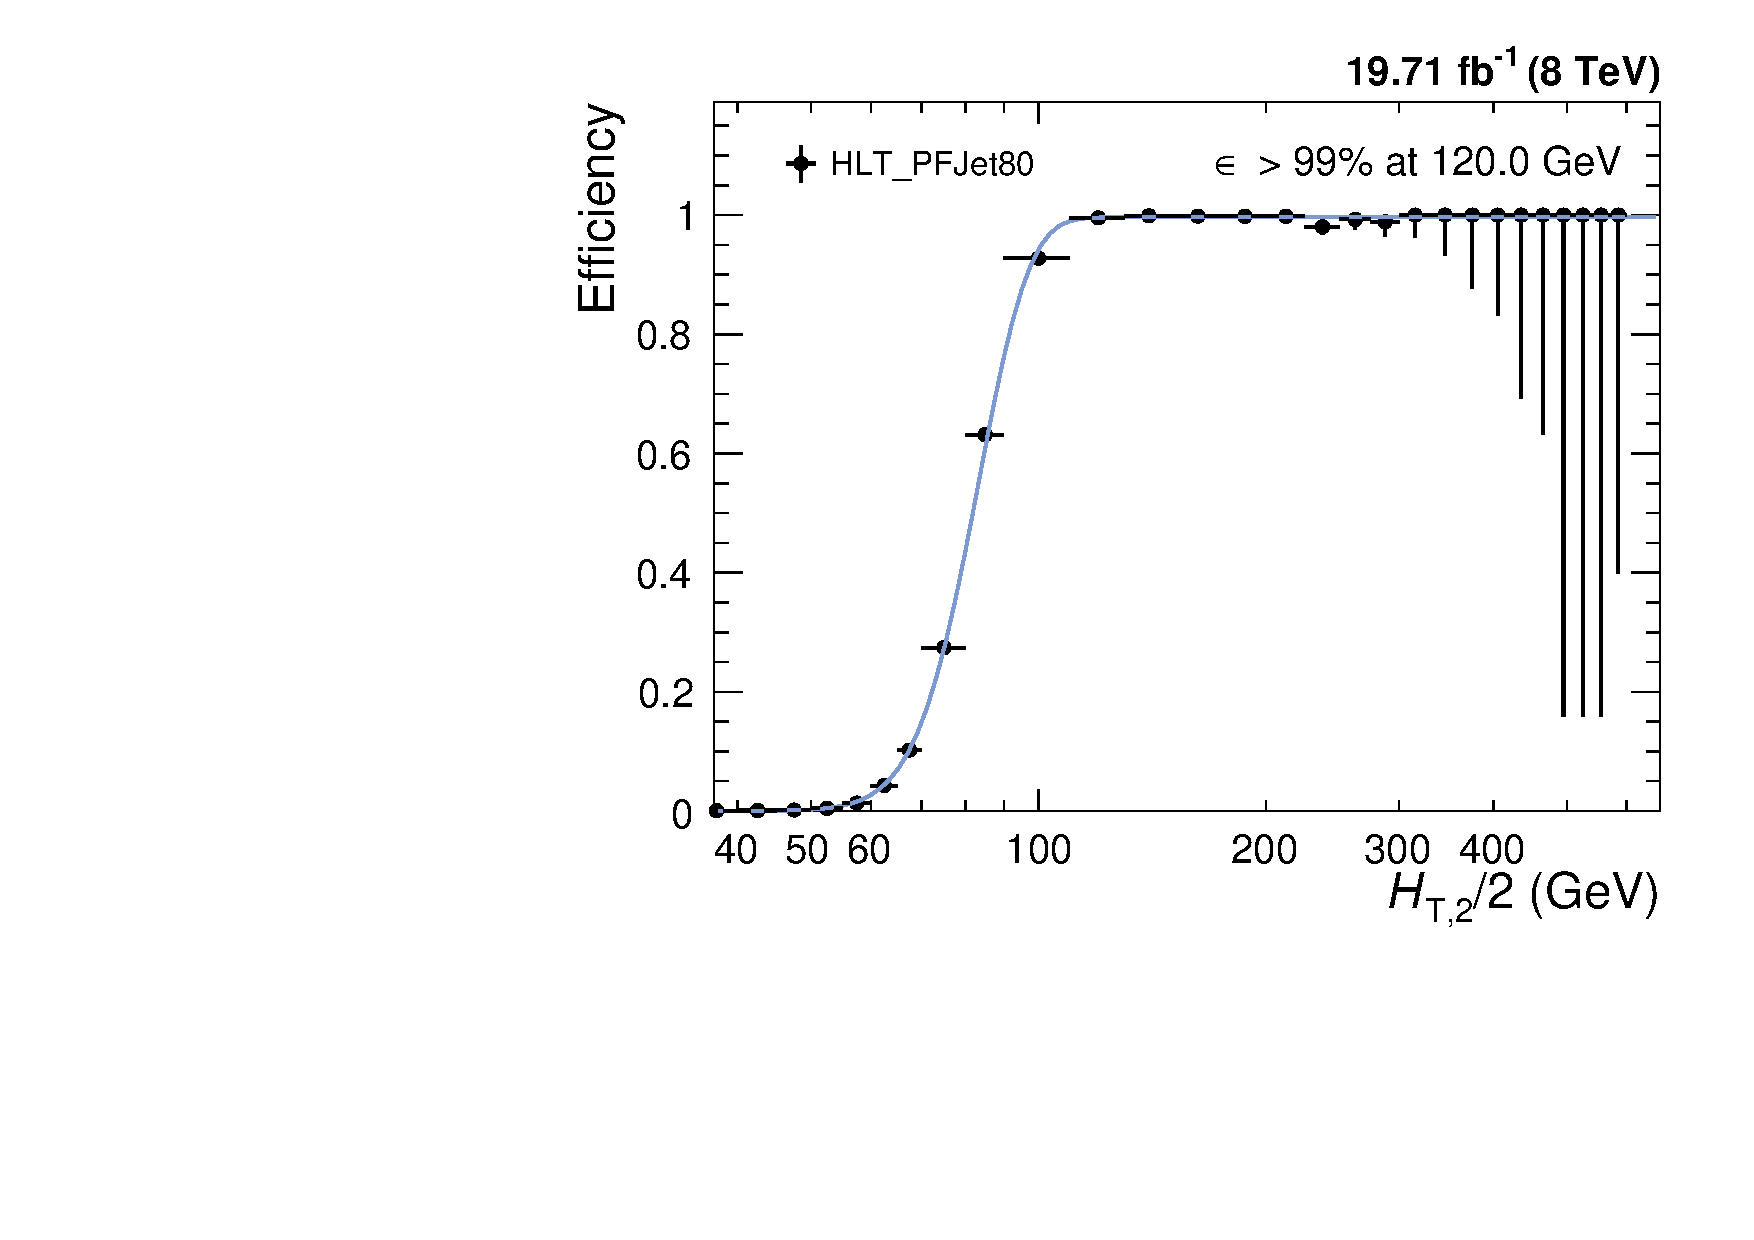
\includegraphics[width=0.53\textwidth]{Plots_HT_2_150/Fit_Turn_Efficiency_80_2_ht_2.pdf}%
 ~~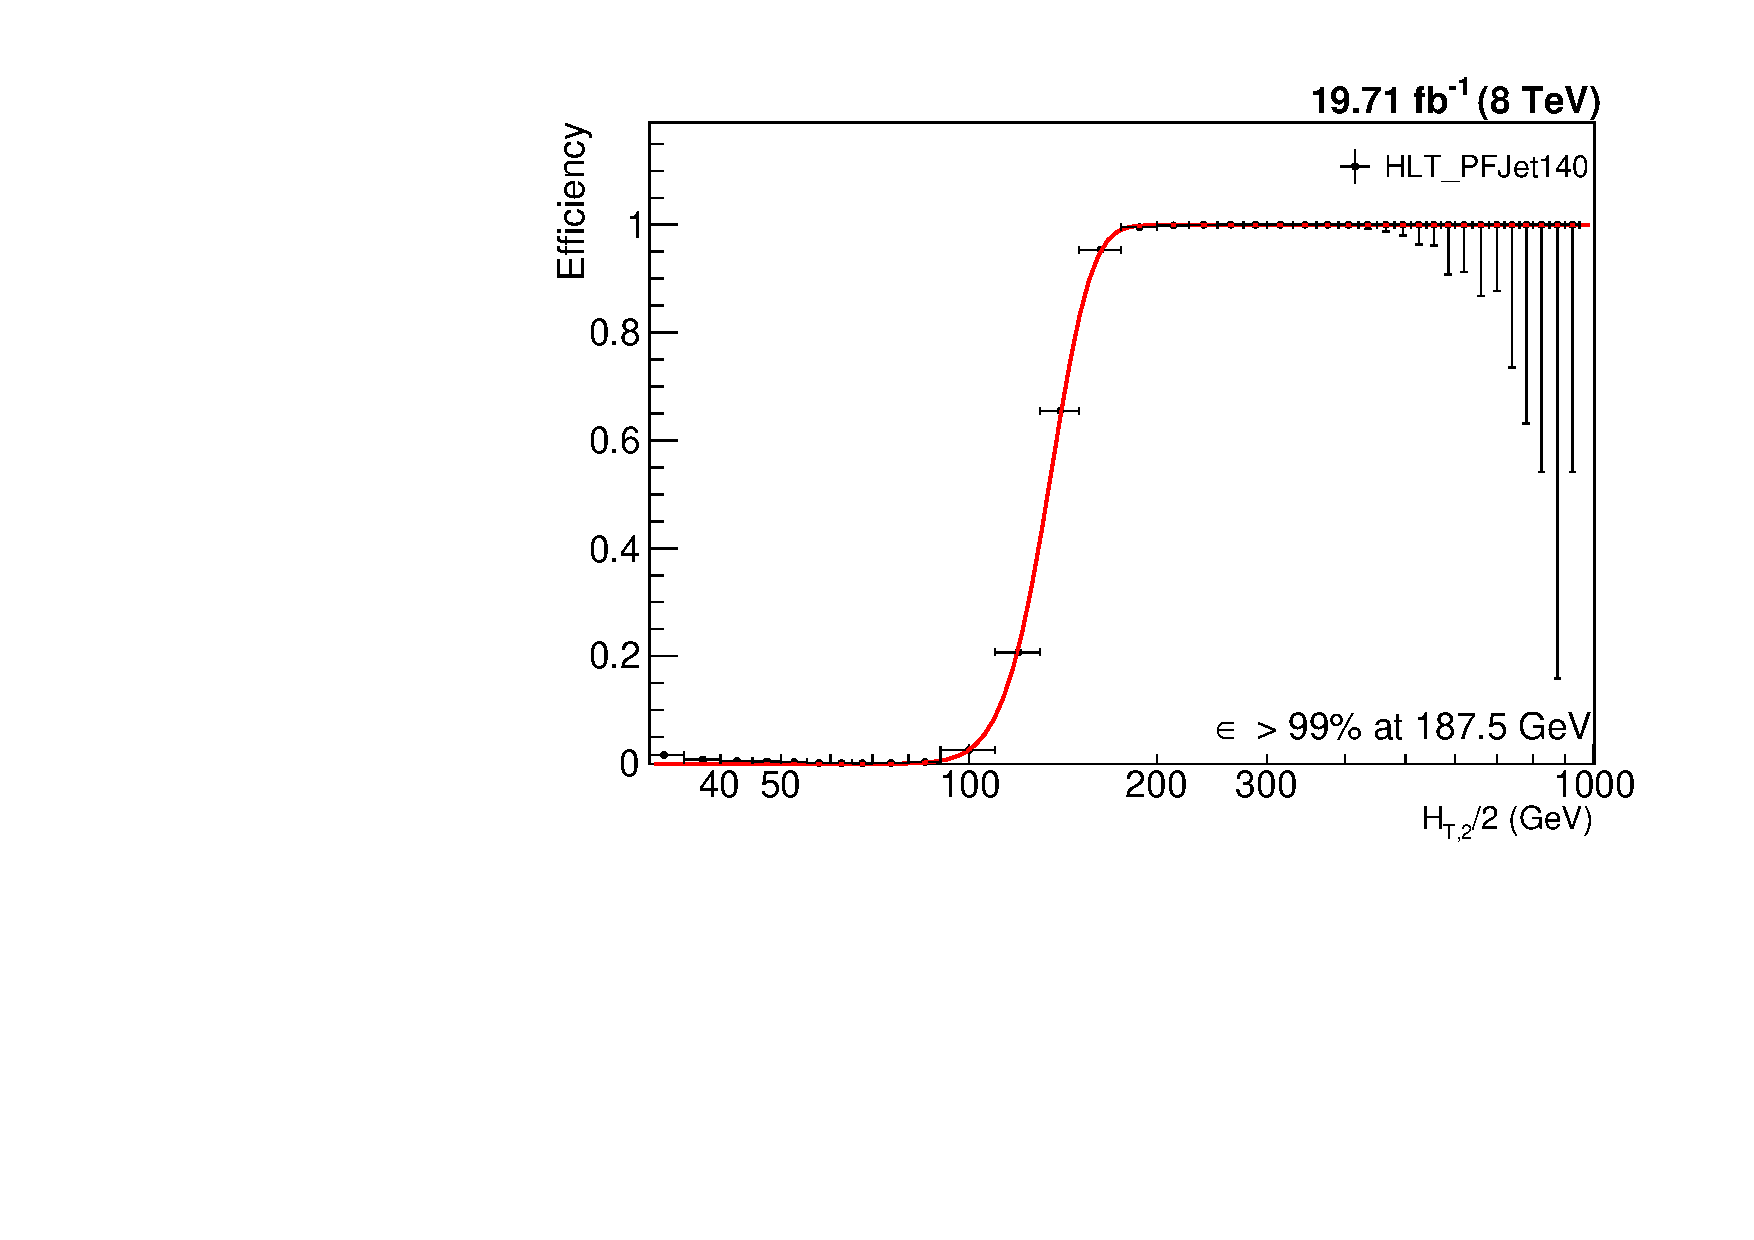
\includegraphics[width=0.53\textwidth]{Plots_HT_2_150/Fit_Turn_Efficiency_140_2_ht_2.pdf}\\
 \hspace*{-10mm}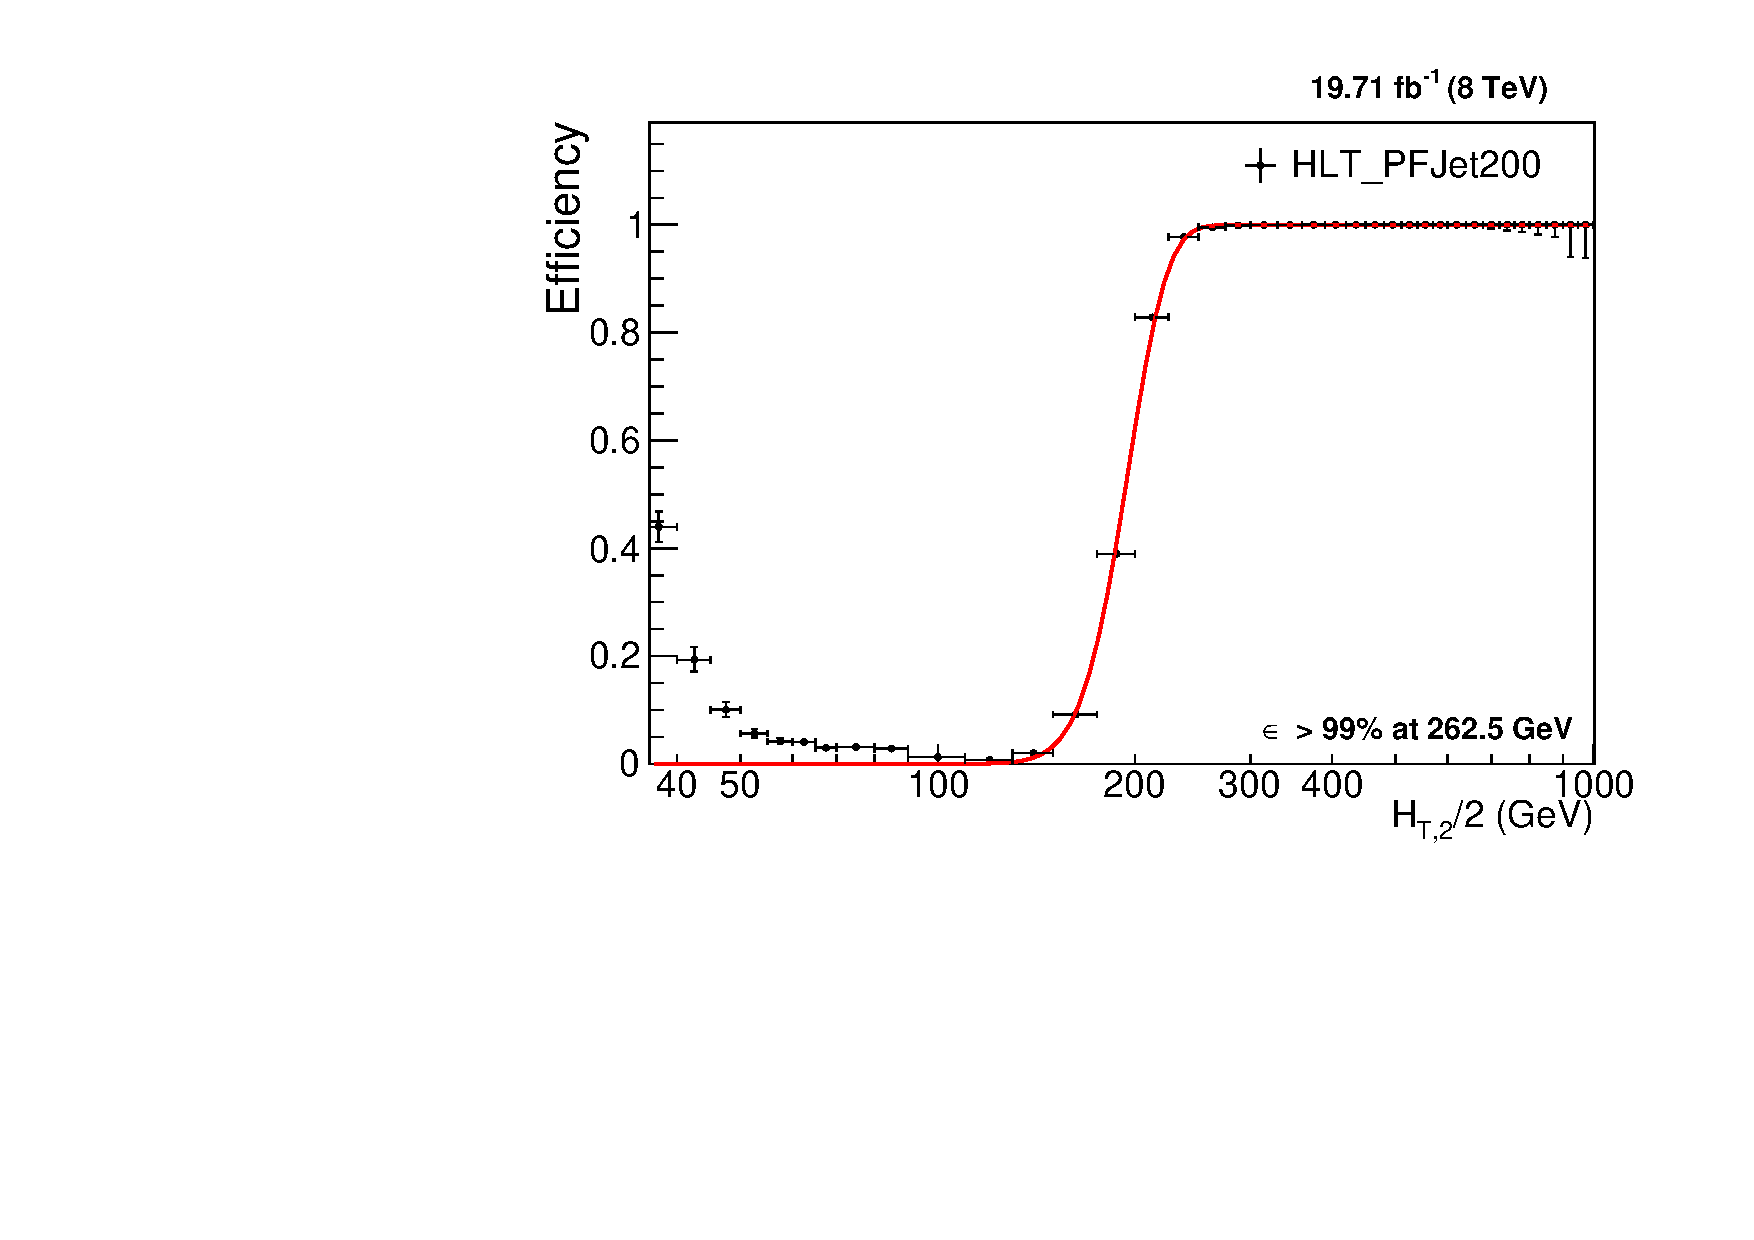
\includegraphics[width=0.53\textwidth]{Plots_HT_2_150/Fit_Turn_Efficiency_200_2_ht_2.pdf}%
 ~~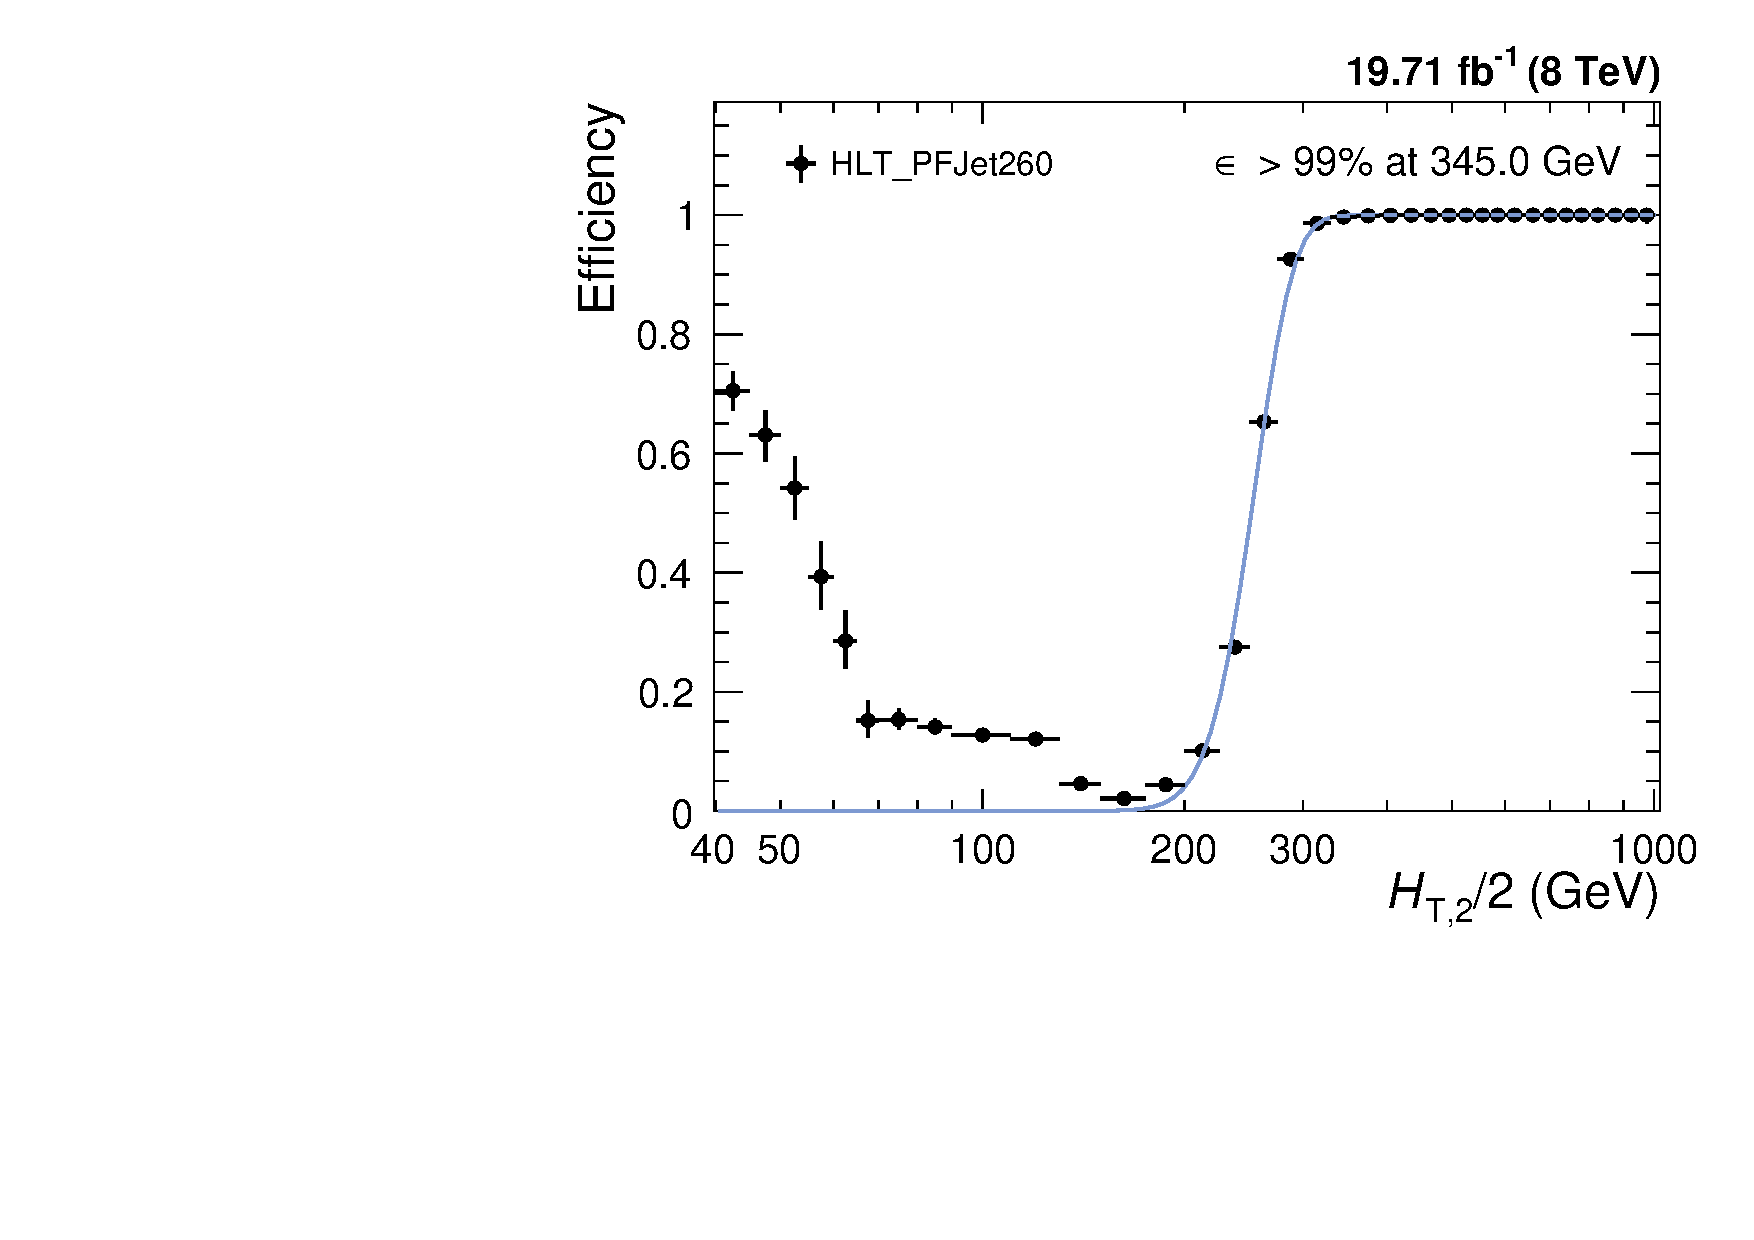
\includegraphics[width=0.53\textwidth]{Plots_HT_2_150/Fit_Turn_Efficiency_260_2_ht_2.pdf}\\
 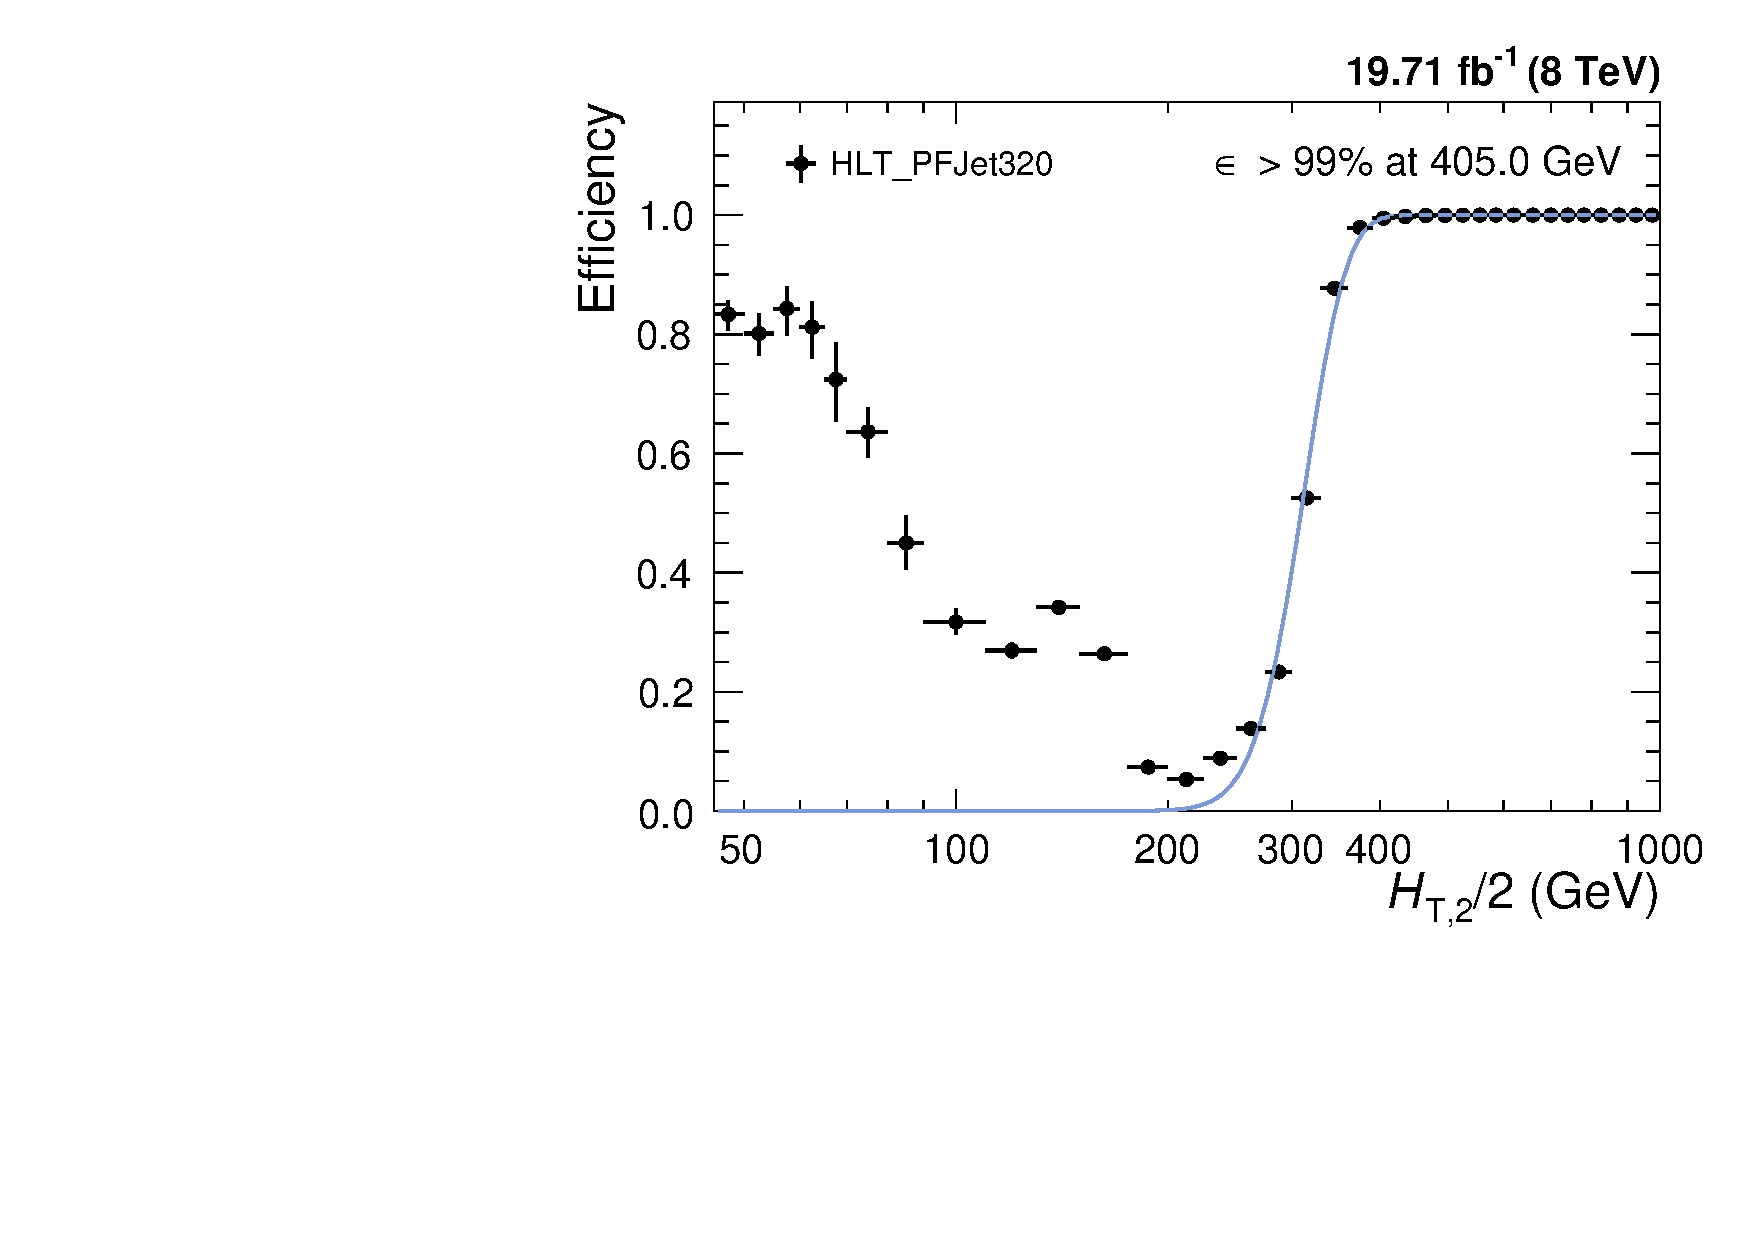
\includegraphics[width=0.53\textwidth]{Plots_HT_2_150/Fit_Turn_Efficiency_320_2_ht_2.pdf}
 \caption[Trigger efficiencies turn-on curves for the single jet HLT trigger paths.]{Trigger efficiencies turn-on curves for the single jet HLT trigger paths are fitted with a sigmoid function (blue line) to obtain the 99\% efficiency threshold. The error bars give the uncertainty on the efficiency which is calculated using Clopper-Pearson confidence intervals \cite{10.2307/2331986}.}
 \label{fig:trig_eff}
 \end{center}
\end{figure}

\subsection{Primary Vertex Selection}
The reconstructed tracks, number of strip and pixel hits and the normalized track \chisq, identify the primary vertex (PV). The tracks are clustered according to the z-coordinate of their point of closest approach to the beam axis. A selection criteria for primary vertex should be followed which helps to identify and reject the beam background events. At-least one good primary vertex reconstructed from at least four tracks within a distance of \abs{z(PV)}\ls 24 cm to the nominal interaction point in a collision, is required in each event. The radial distance in x-y plane, $\rho$(PV) should be not be greater than 2 cm. The number of degrees of freedom in fitting for the position of each vertex using its associated tracks should be at-least four in number. 

\subsection{Missing Transverse Energy}
In an ideal detector where all particles could be identified and perfectly measured, the transverse momentum of all particles would sum up to zero. But the neutral weakly interacting particles, such as neutrinos, escape from typical collider detectors and do not produce any direct response in the detector elements. The imbalance of total momentum of all visible particles can give the hints of the presence of such particles. The vector momentum imbalance in the plane perpendicular to the beam direction is known as missing transverse momentum or energy (\ETmiss). It is one of the most important observables for discriminating leptonic decays of W bosons and top quarks from background events which do not contain neutrinos, such as multijet and Drell–Yan events or searches for physics beyond the Standard Model.

The ratio of missing transverse energy to the total transverse energy \ETmiss/$\sum\ET$, shown in Fig.~\ref{fig:metcut} for \njt~(left) and \njth~events (right), shows a discrepancy between data (black solid circles) and simulated MC (blue histogram), at the tail part of the distribution. This is because of a finite contribution from Z($\rightarrow \nu \bar{\nu}$) \plus jet events which gives rise to non-zero \ET in the events in data. Such events are absent in QCD simulated events in MC. Hence \ETmiss/$\sum\ET$ is required to be less than 0.3 to reject events with high \ETmiss.

\begin{figure}[!htbp]
\centering
 \hspace*{-2mm}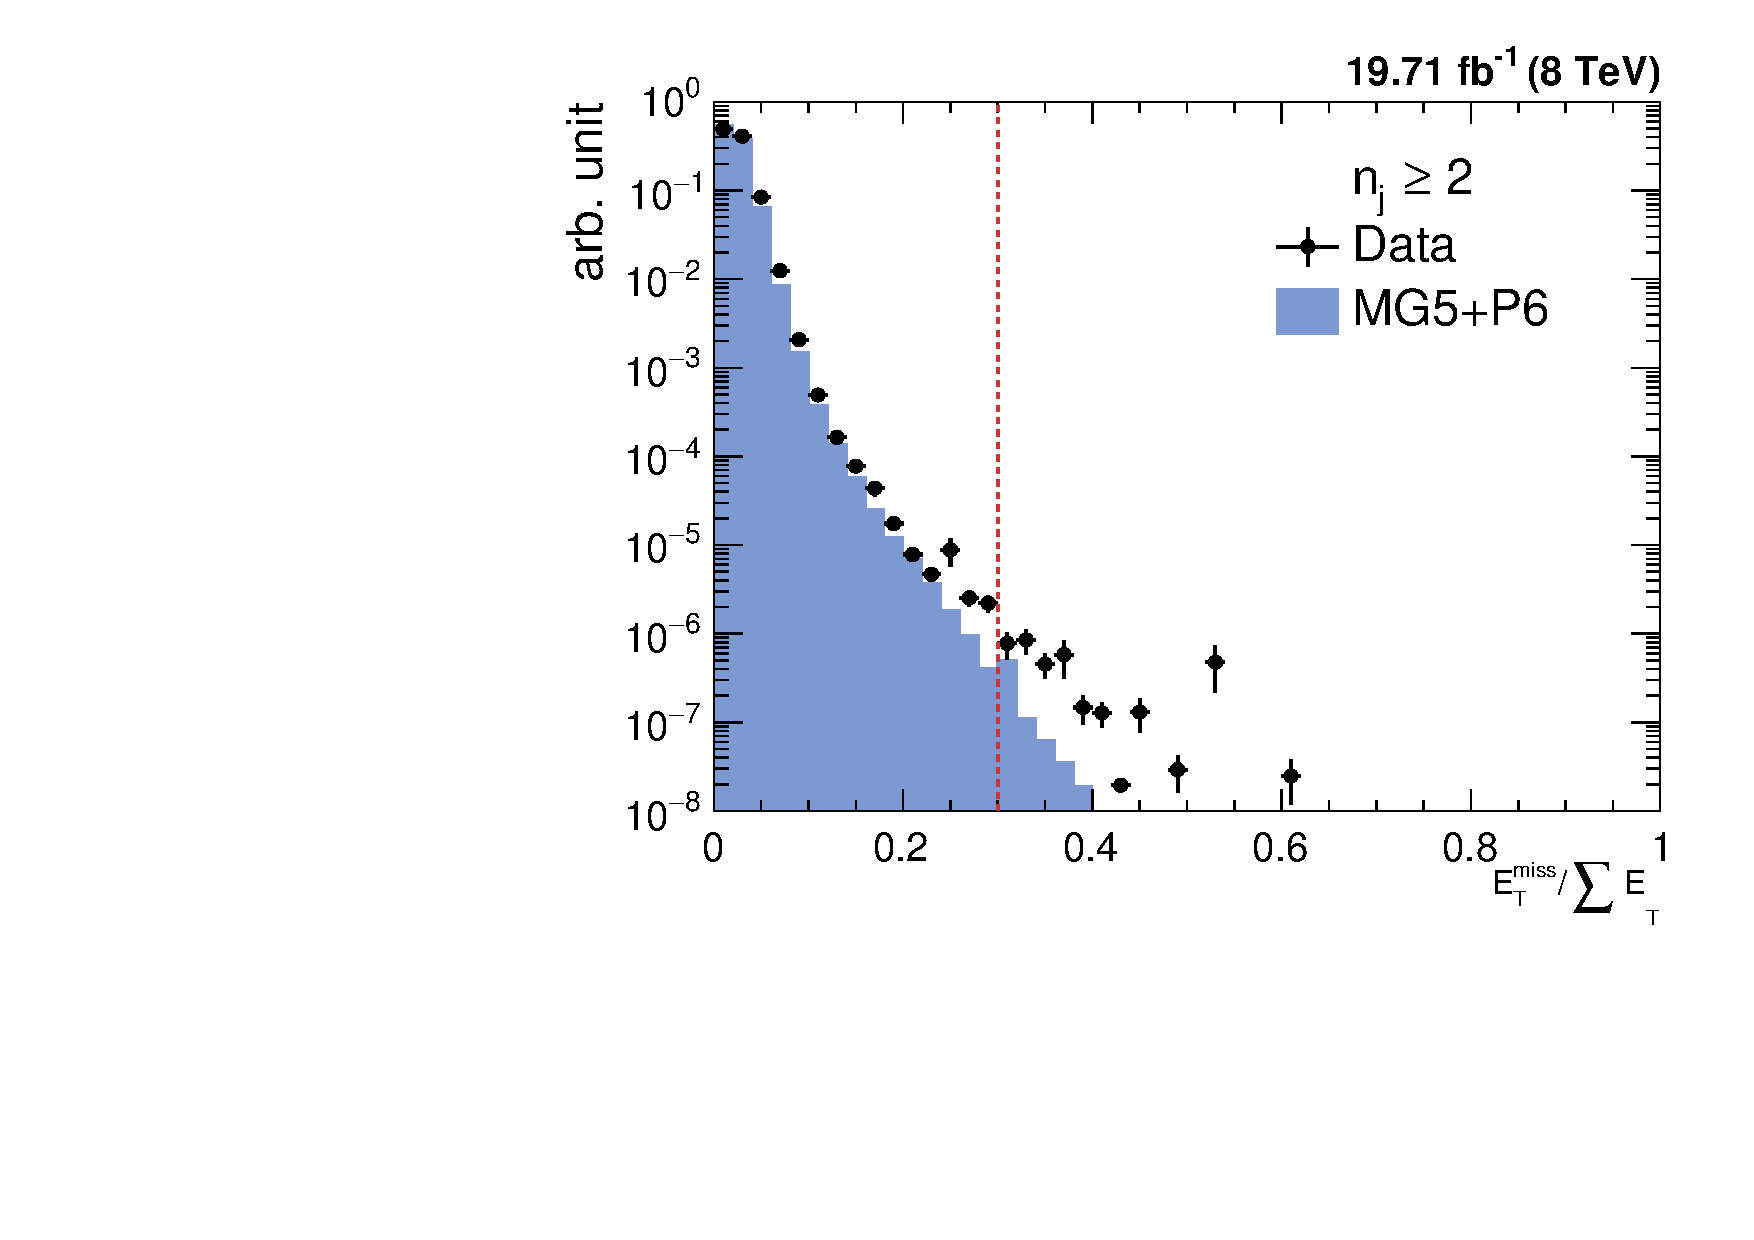
\includegraphics[width=0.51\textwidth]{Plots_HT_2_150/Missing_ET_2.pdf}%
 ~~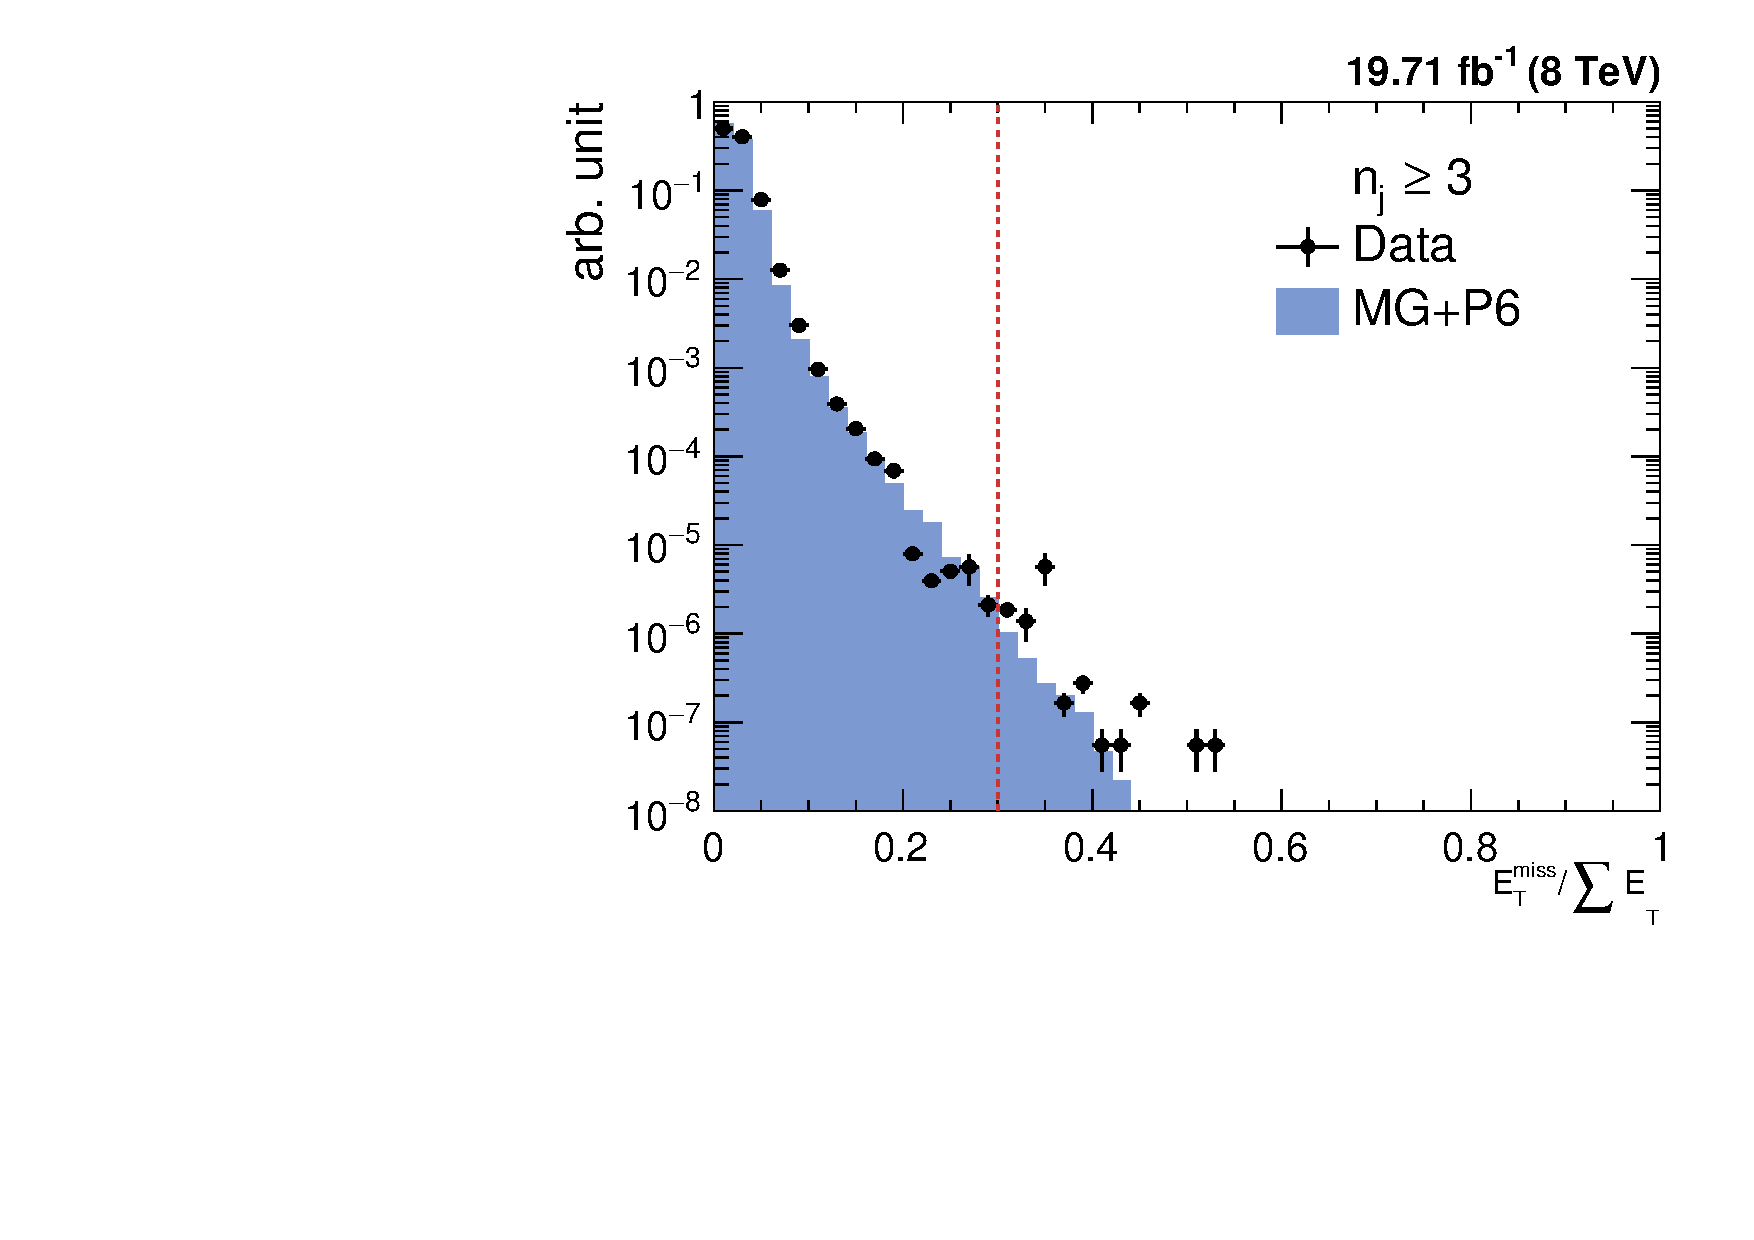
\includegraphics[width=0.51\textwidth]{Plots_HT_2_150/Missing_ET_3.pdf}
 \caption[Missing transverse energy fraction of the total transverse energy per event in data and simulated Monte Carlo events.]{Missing transverse energy fraction of the total transverse energy per event in data (black solid circles) and simulated Monte Carlo events (blue histogram) in inclusive 2-jet (left) and 3-jet events (right). To remove background and noise, events with a fraction exceeding a certain threshold, here indicated with the red dashed line, are rejected.}
 \label{fig:metcut}
\end{figure} 

\subsection{Jet Identification}
In order to suppress fake jets, arising from detector noise or misreconstructed particles, jet identification criteria (ID) has been applied. Instead of applying it event-wise, it is applied it on each jet. The algorithm works on reconstructed jets using information of the clustered particle candidates. The official tight jet ID \cite{CMS:2010xta}, recommended by \JetMet group \cite{JetID} is used. Due to pileup and electronic noise the jet constituent fractions may vary from event to event. In order to reject the noisy jets, some jet selection criteria are optimized to select only good quality jets. The selection criteria are implemented as selection cut on jet fractions. Table~\ref{tab:jetID} summarizes the properties of the reconstructed jets and their respective cuts. Each jet should contain at least two particles, one of which should be a charged hadron. The cut on the fraction of neutral hadrons and photons removes HCAL noise and ECAL noise, respectively. Muons that are falsely identified and clustered as jets are removed by the muon fraction criterion. Based on information of the tracker, additional selection cuts are enforced in the region $|\eta|$ \ls 2.4. The charged electromagnetic fraction cut removes the jets clustered from misidentified electrons. Furthermore, the fraction of charged hadrons in the jet must be larger than zero and jets without any charged hadrons are very likely to be pileup jets. The Figs.~\ref{fig:qual2} and~\ref{fig:qual3} show the distributions of the jet constituents observed in data (black solid circles) and simulated MC events (blue histogram) for \njt~and \njth, respectively.

\begin{table}[!htbp]
 \centering
 \caption[The jet ID removes noise and fake jets based on the properties of the reconstructed jets and the clustered particle candidates.]{The jet ID removes noise and fake jets based on the properties of the reconstructed jets and the clustered particle candidates. All the selection cuts which are recommended by the \JetMet group are applied \cite{JetID}.}
 \label{tab:jetID}
 \vspace{2mm}
 \begin{tabular}{llll}
 \hline\hline
 \centering
                      & {\bf Property}          & {\bf Loose ID} & {\bf Tight ID} \rbthm\\\hline
                      & neutral hadron fraction & \ls 0.99       & \ls 0.90       \rbtrr \\
  Whole               & neutral EM fraction     & \ls 0.99       & \ls 0.90       \rbtrr \\
 $\eta$ region        & number of constituents  & \gr 1          & \gr 1          \rbtrr \\
                      & muon fraction           & \ls 0.80       & \ls 0.80       \rbtrr \\ \hline
                      & charged hadron fraction & \gr 0          & \gr 0          \rbtrr \\
only $|\eta|$ \ls 2.4 & charged multiplicity    & \gr 0          & \gr 0          \rbtrr \\
                      & charged EM fraction     & \ls 0.99       & \ls 0.90       \rbtrr \\
 \hline\hline
 \end{tabular}
\end{table}

\begin{figure}[!htbp]
 \begin{center}
 \vspace*{-1mm}
 \hspace*{-2mm}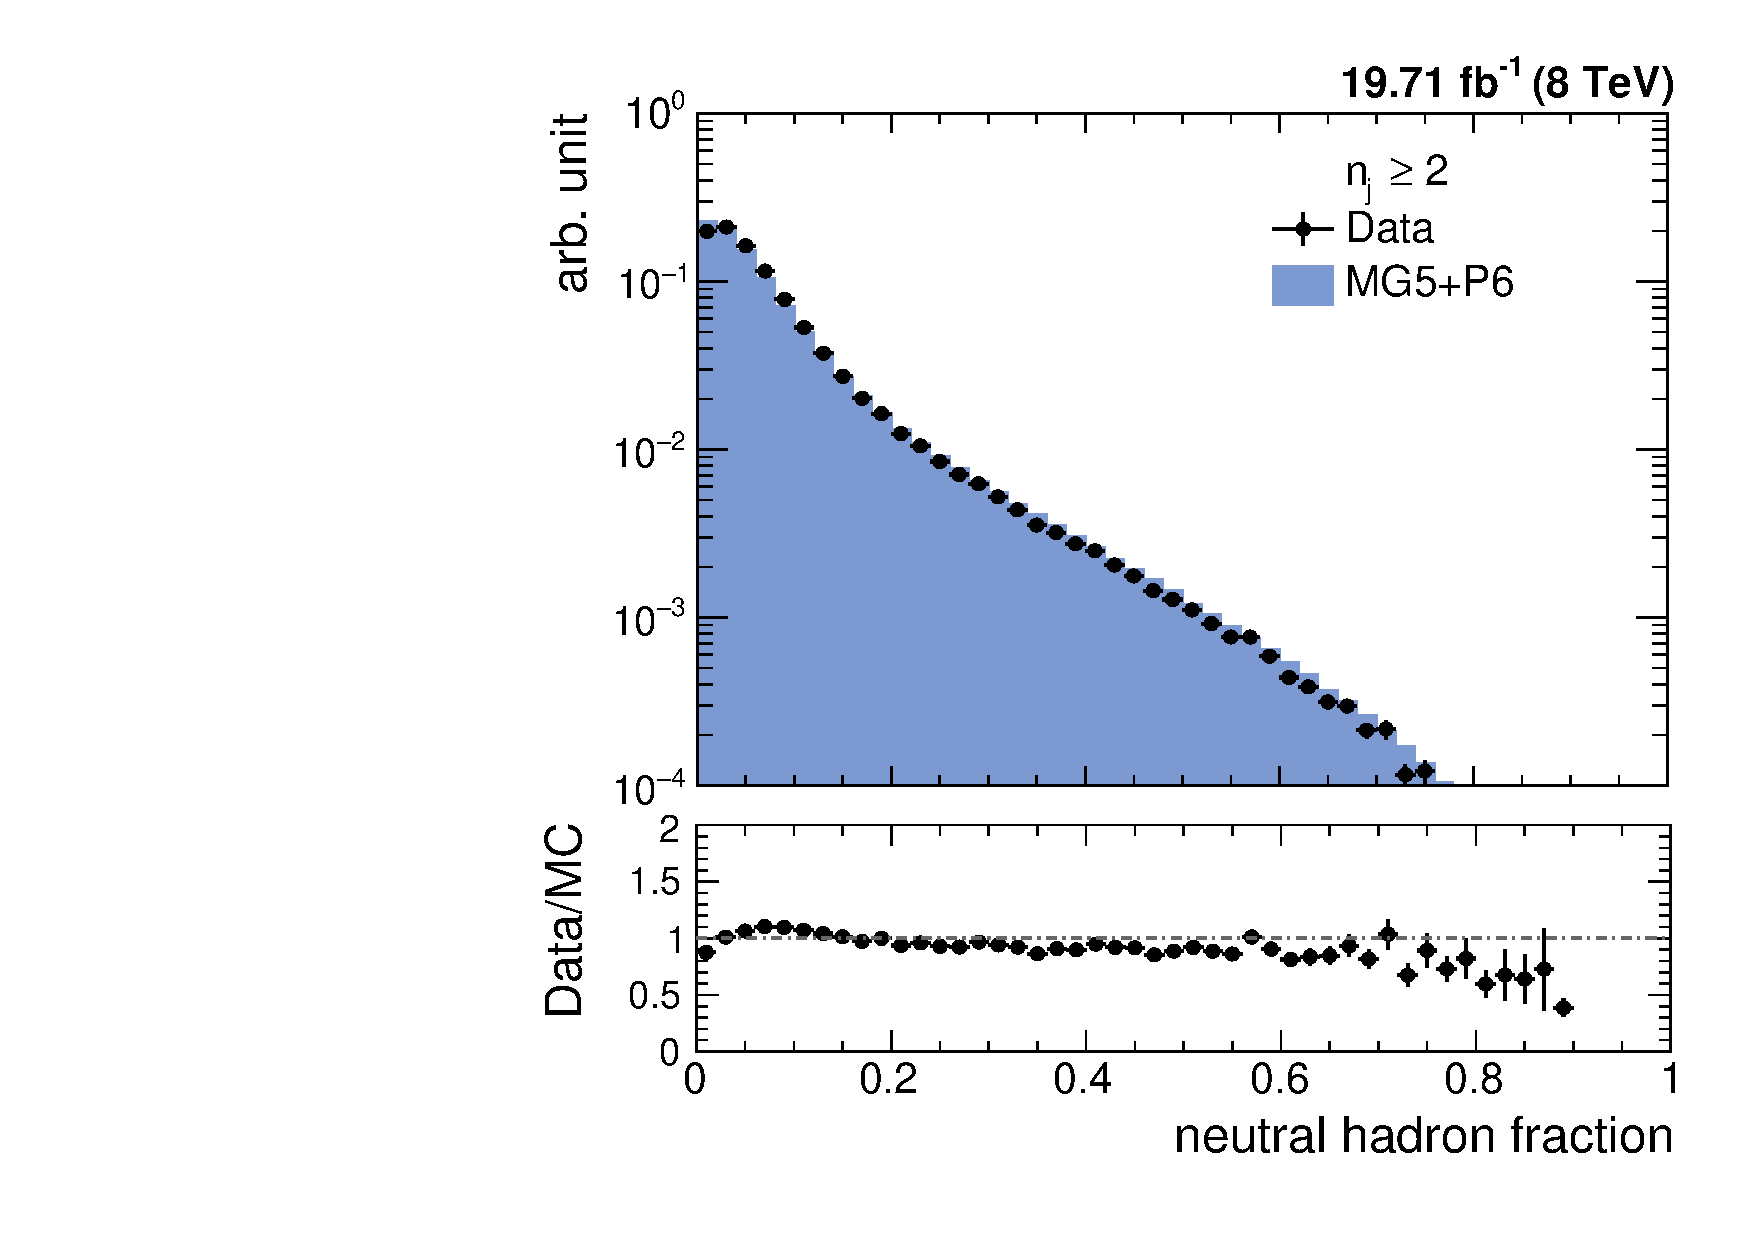
\includegraphics[width=0.51\textwidth]{Plots_HT_2_150/Comparison_NuHadFrac_2_HT_2_150.pdf}%
 ~~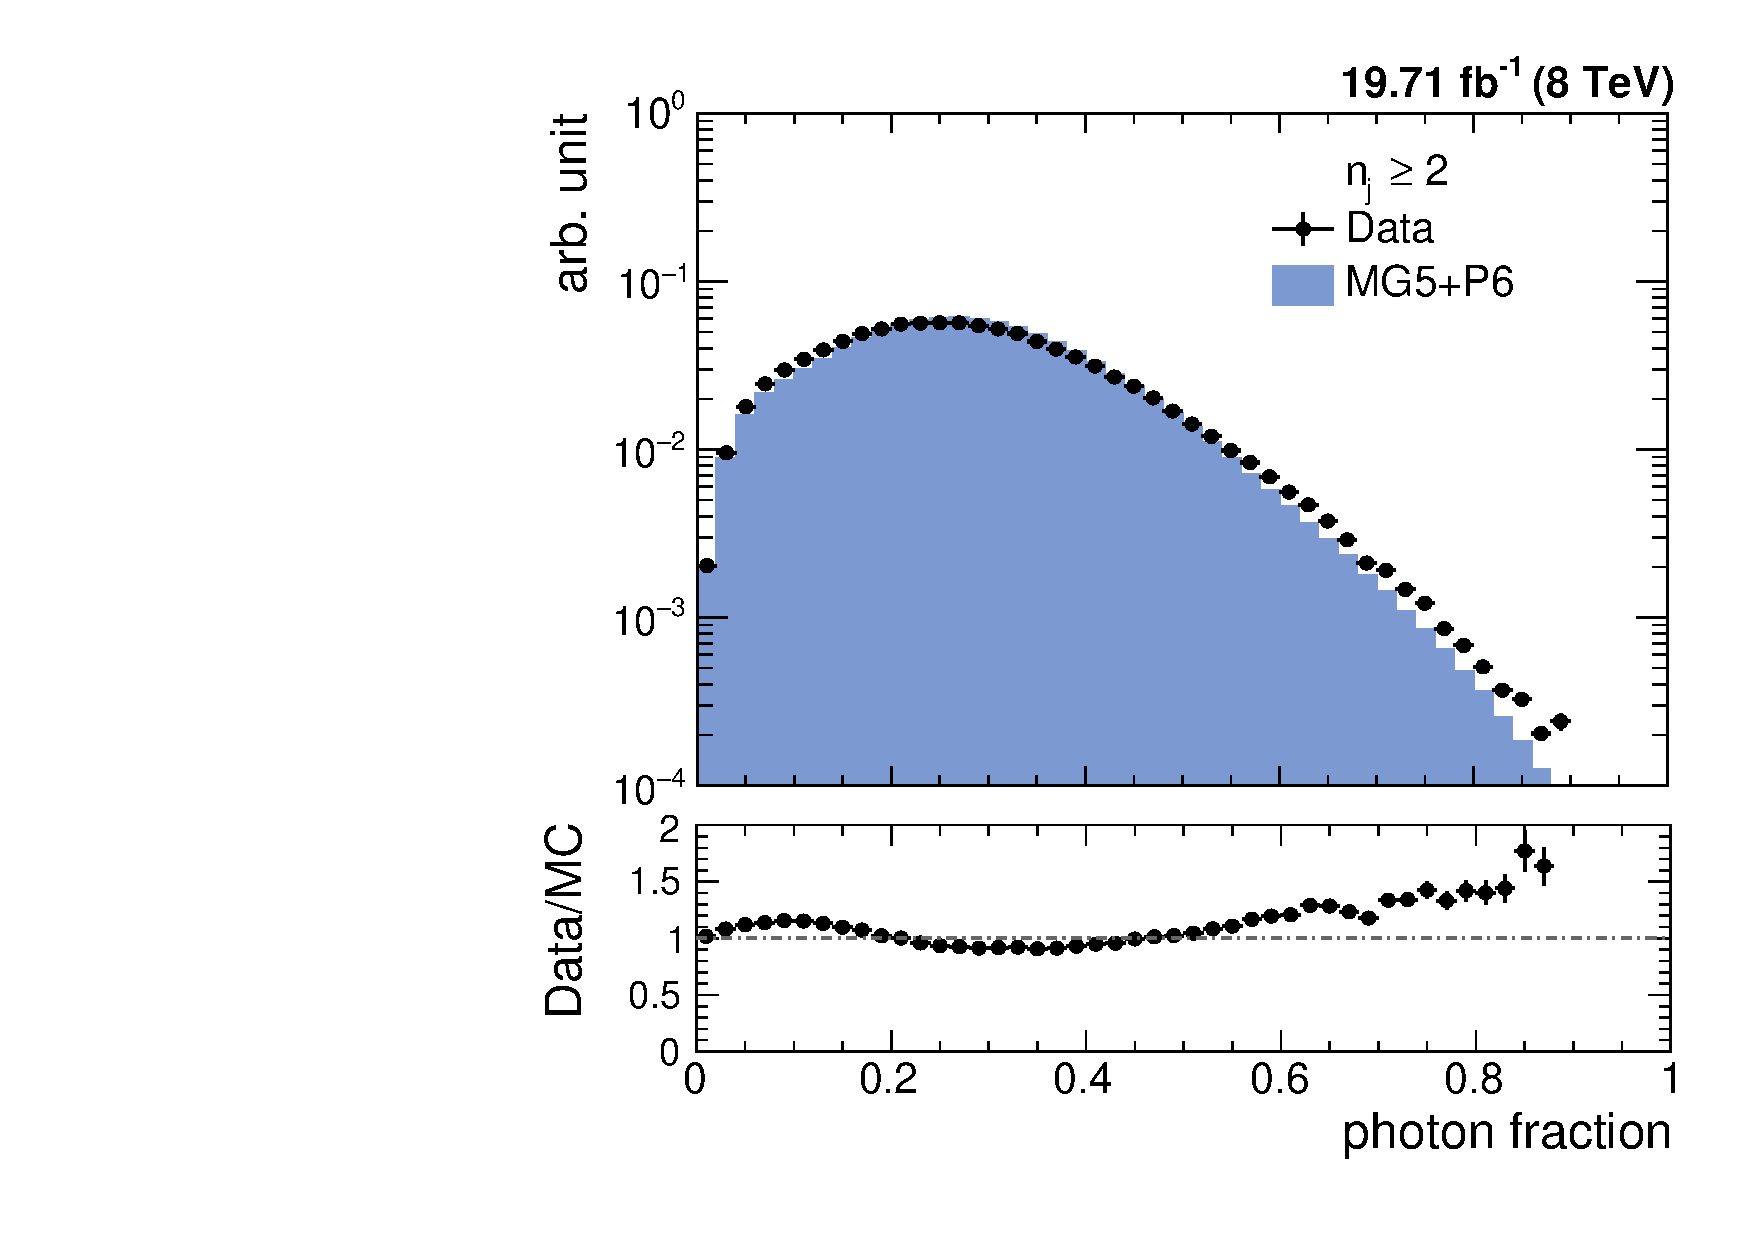
\includegraphics[width=0.51\textwidth]{Plots_HT_2_150/Comparison_PhFrac_2_HT_2_150.pdf}\\
 \vspace*{1mm}
 \hspace*{-2mm}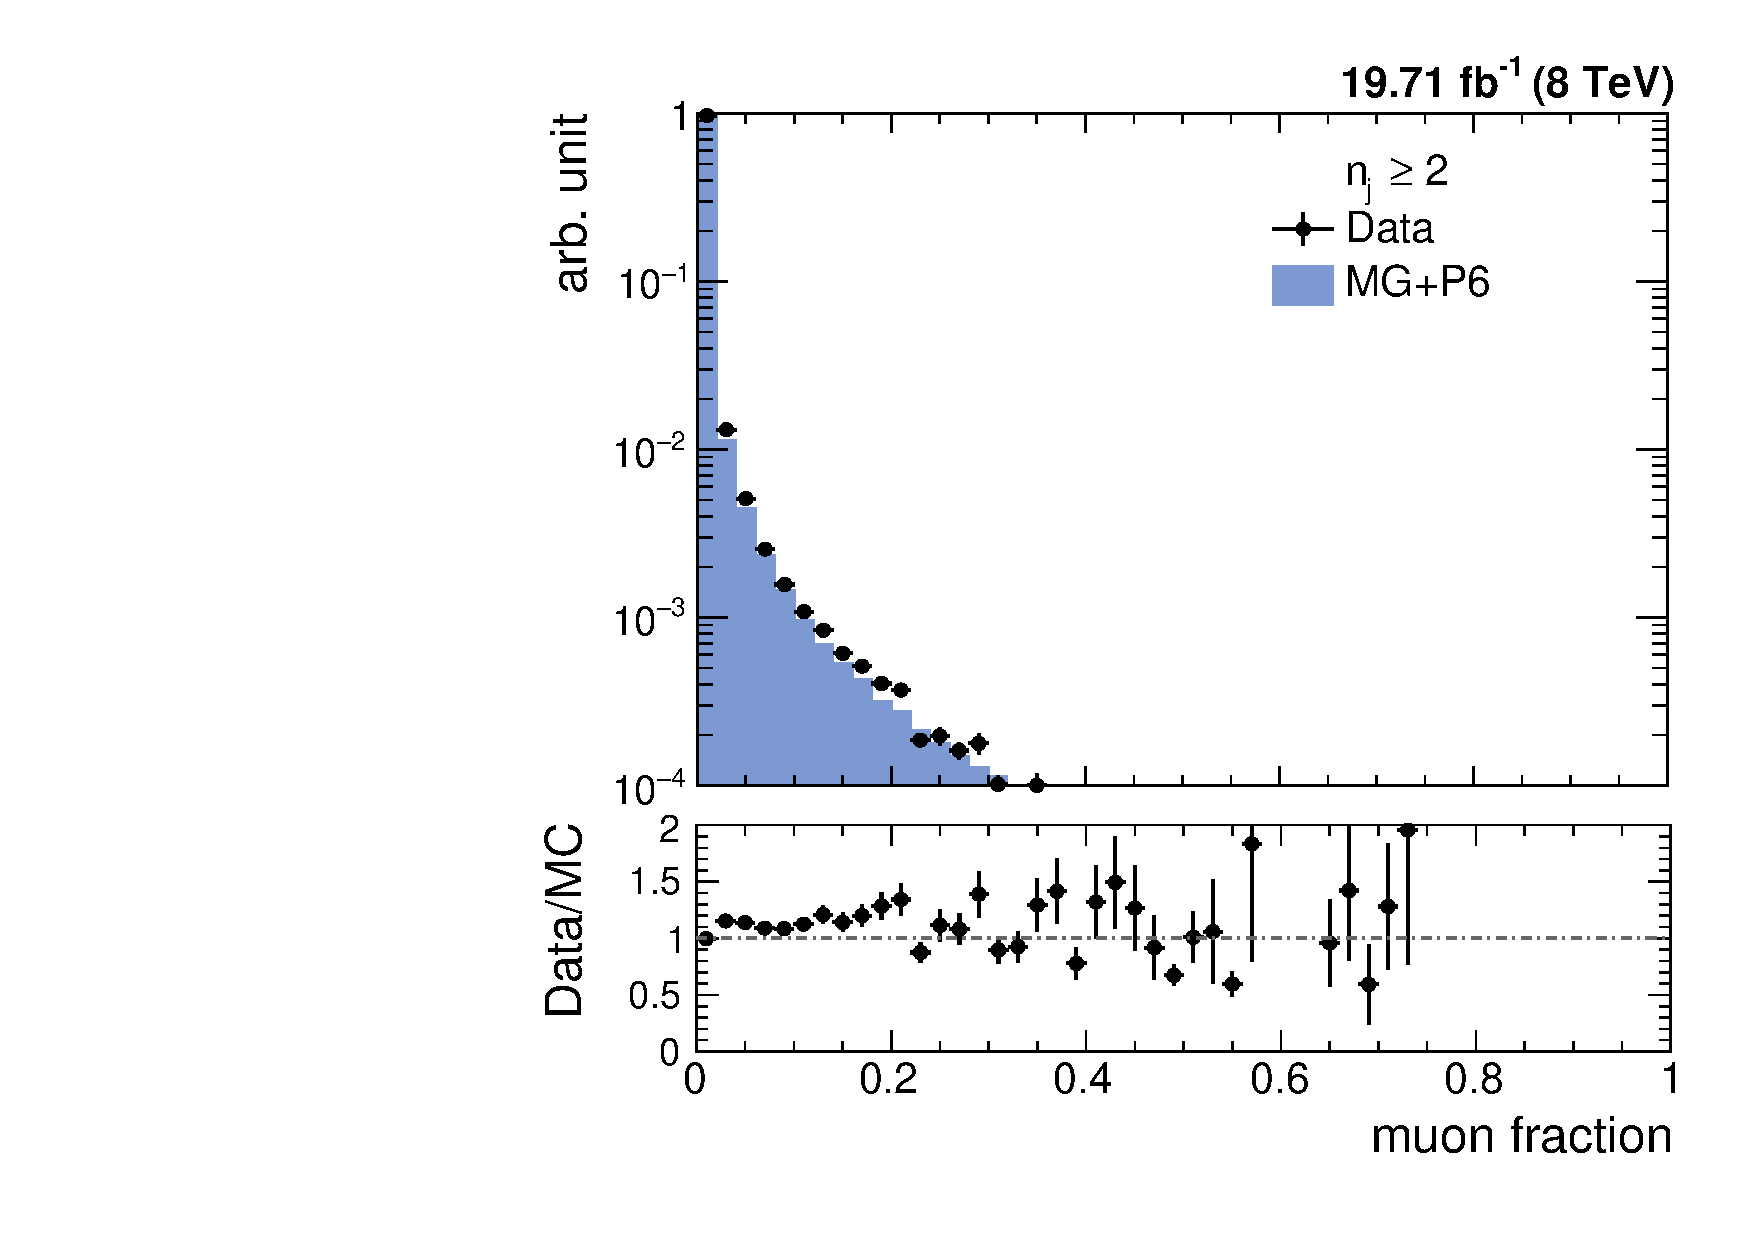
\includegraphics[width=0.51\textwidth]{Plots_HT_2_150/Comparison_MuFrac_2_HT_2_150.pdf}%
 ~~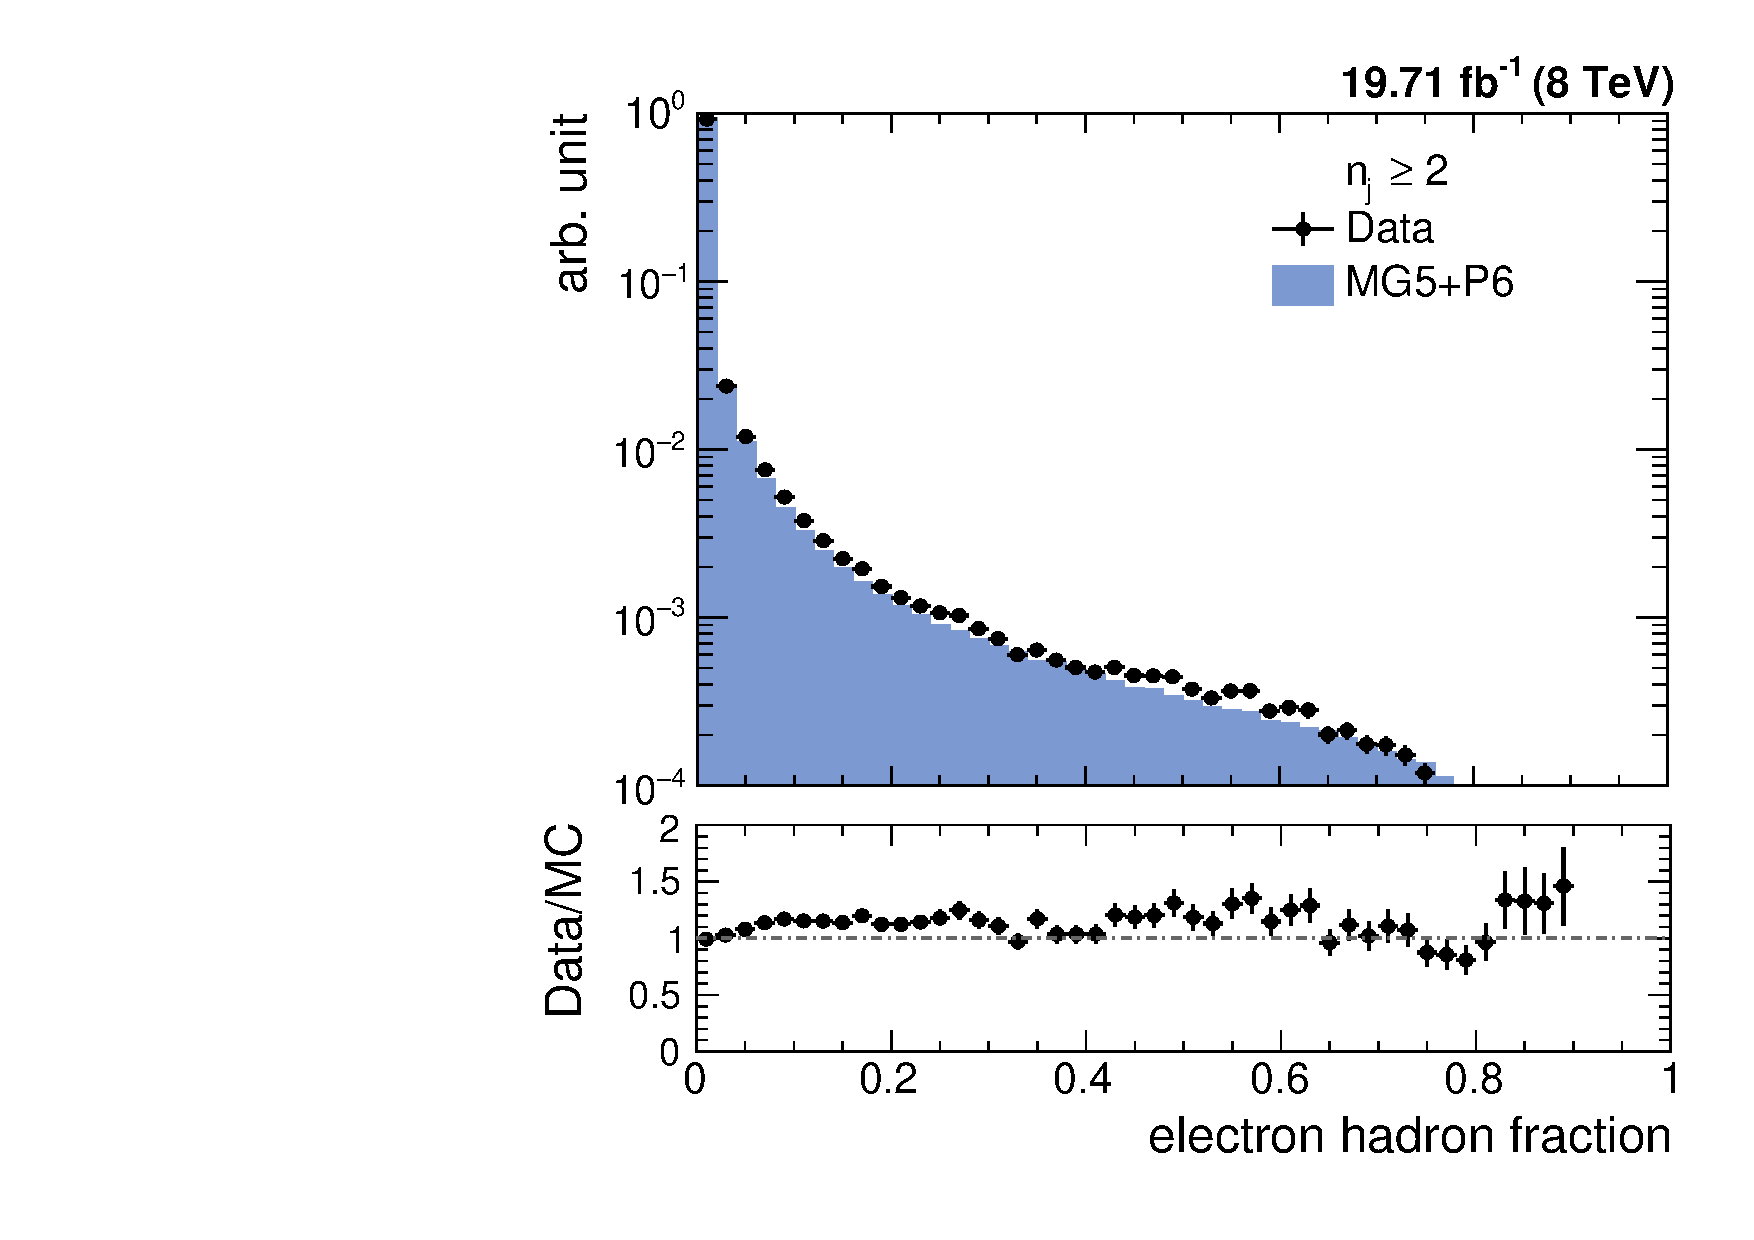
\includegraphics[width=0.51\textwidth]{Plots_HT_2_150/Comparison_ElFrac_2_HT_2_150.pdf}\\
 \vspace*{1mm}
 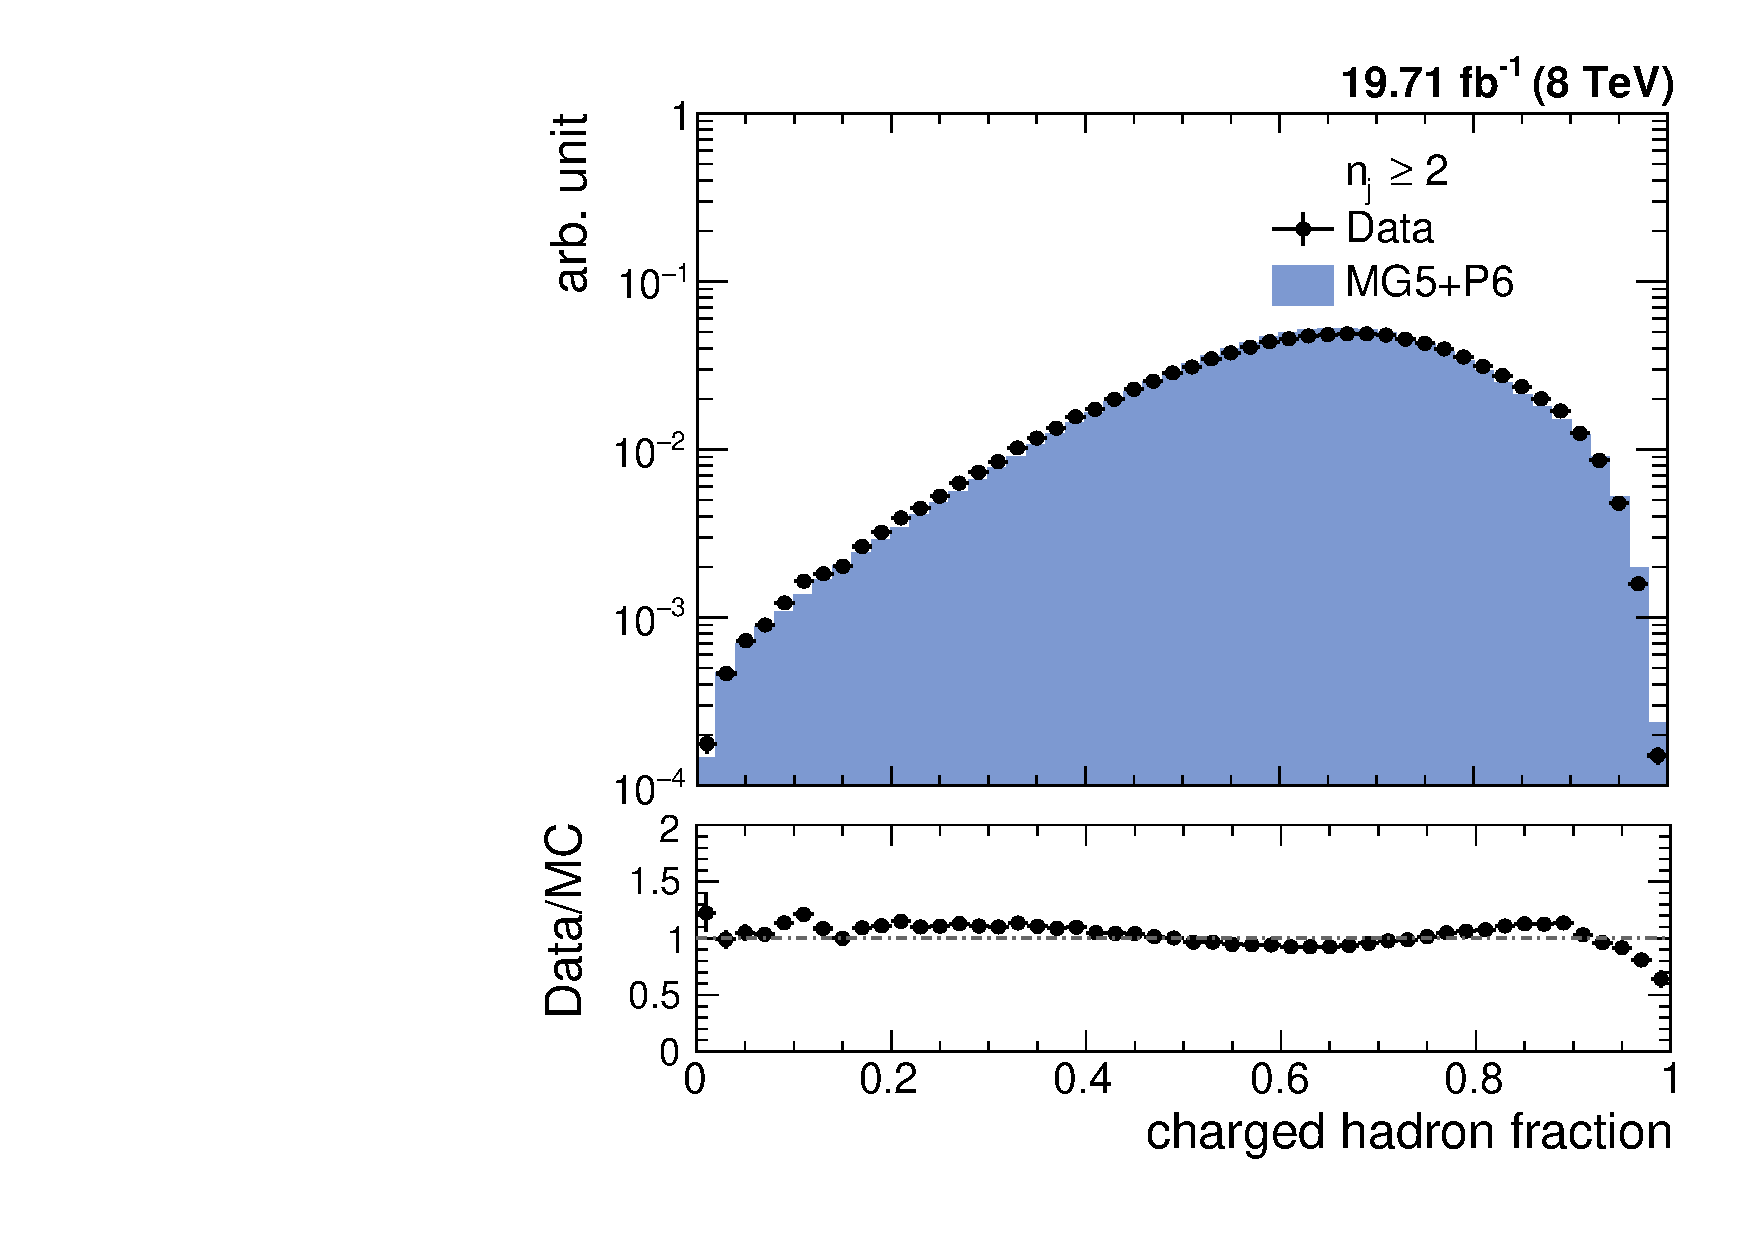
\includegraphics[width=0.51\textwidth]{Plots_HT_2_150/Comparison_ChHadFrac_2_HT_2_150.pdf}
 \caption[The fractions of jet constituents for different types of PF candidates for inclusive 2-jet events.]{The fractions of jet constituents as observed in data (black solid circles) and simulated Monte Carlo events (blue histogram) for different types of PF candidates for inclusive 2-jet events. Data and simulations are normalized to the same number of events. The distributions are shown after the application of the jet ID.}
 \label{fig:qual2}
 \end{center}
\end{figure} 

\begin{figure}[!htbp]
 \begin{center}
 \vspace*{-1mm}
 \hspace*{-2mm}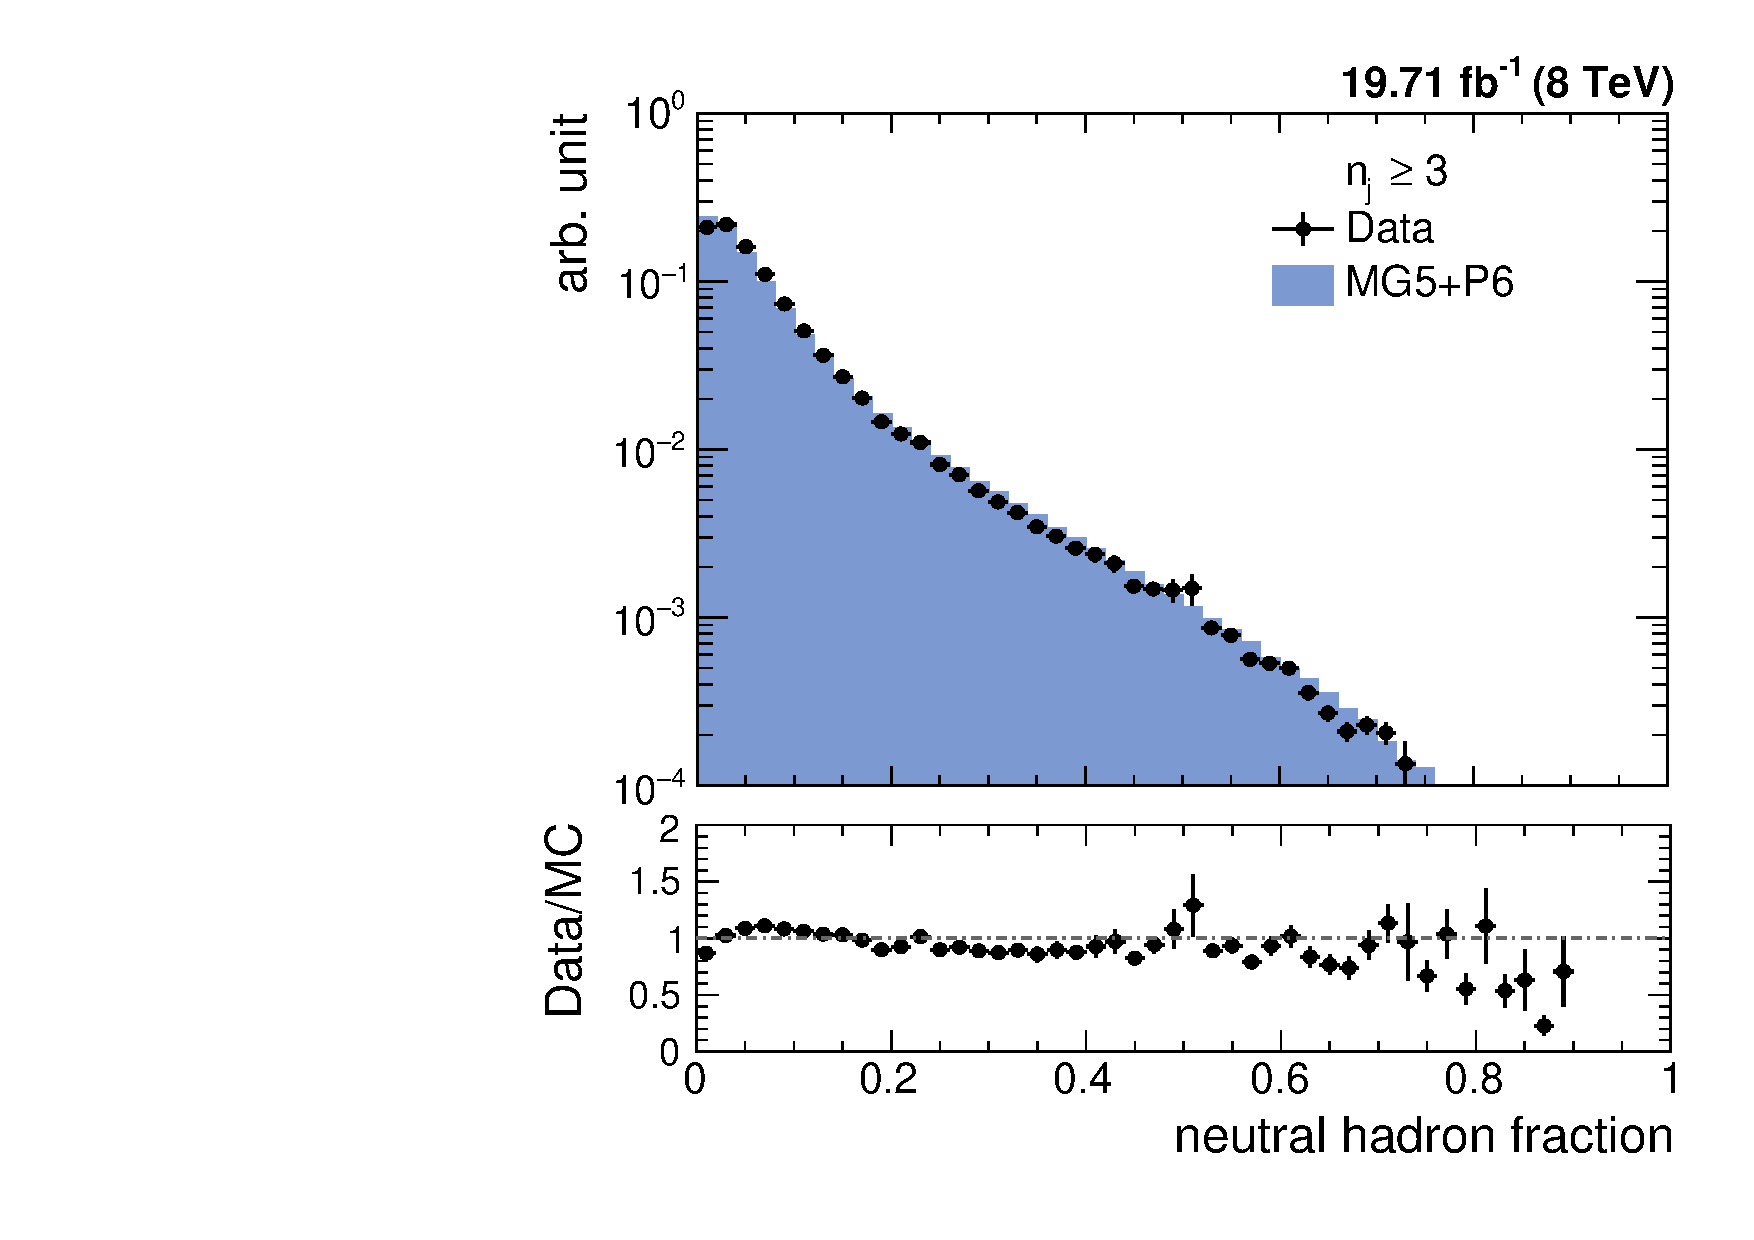
\includegraphics[width=0.51\textwidth]{Plots_HT_2_150/Comparison_NuHadFrac_3_HT_2_150.pdf}%
 ~~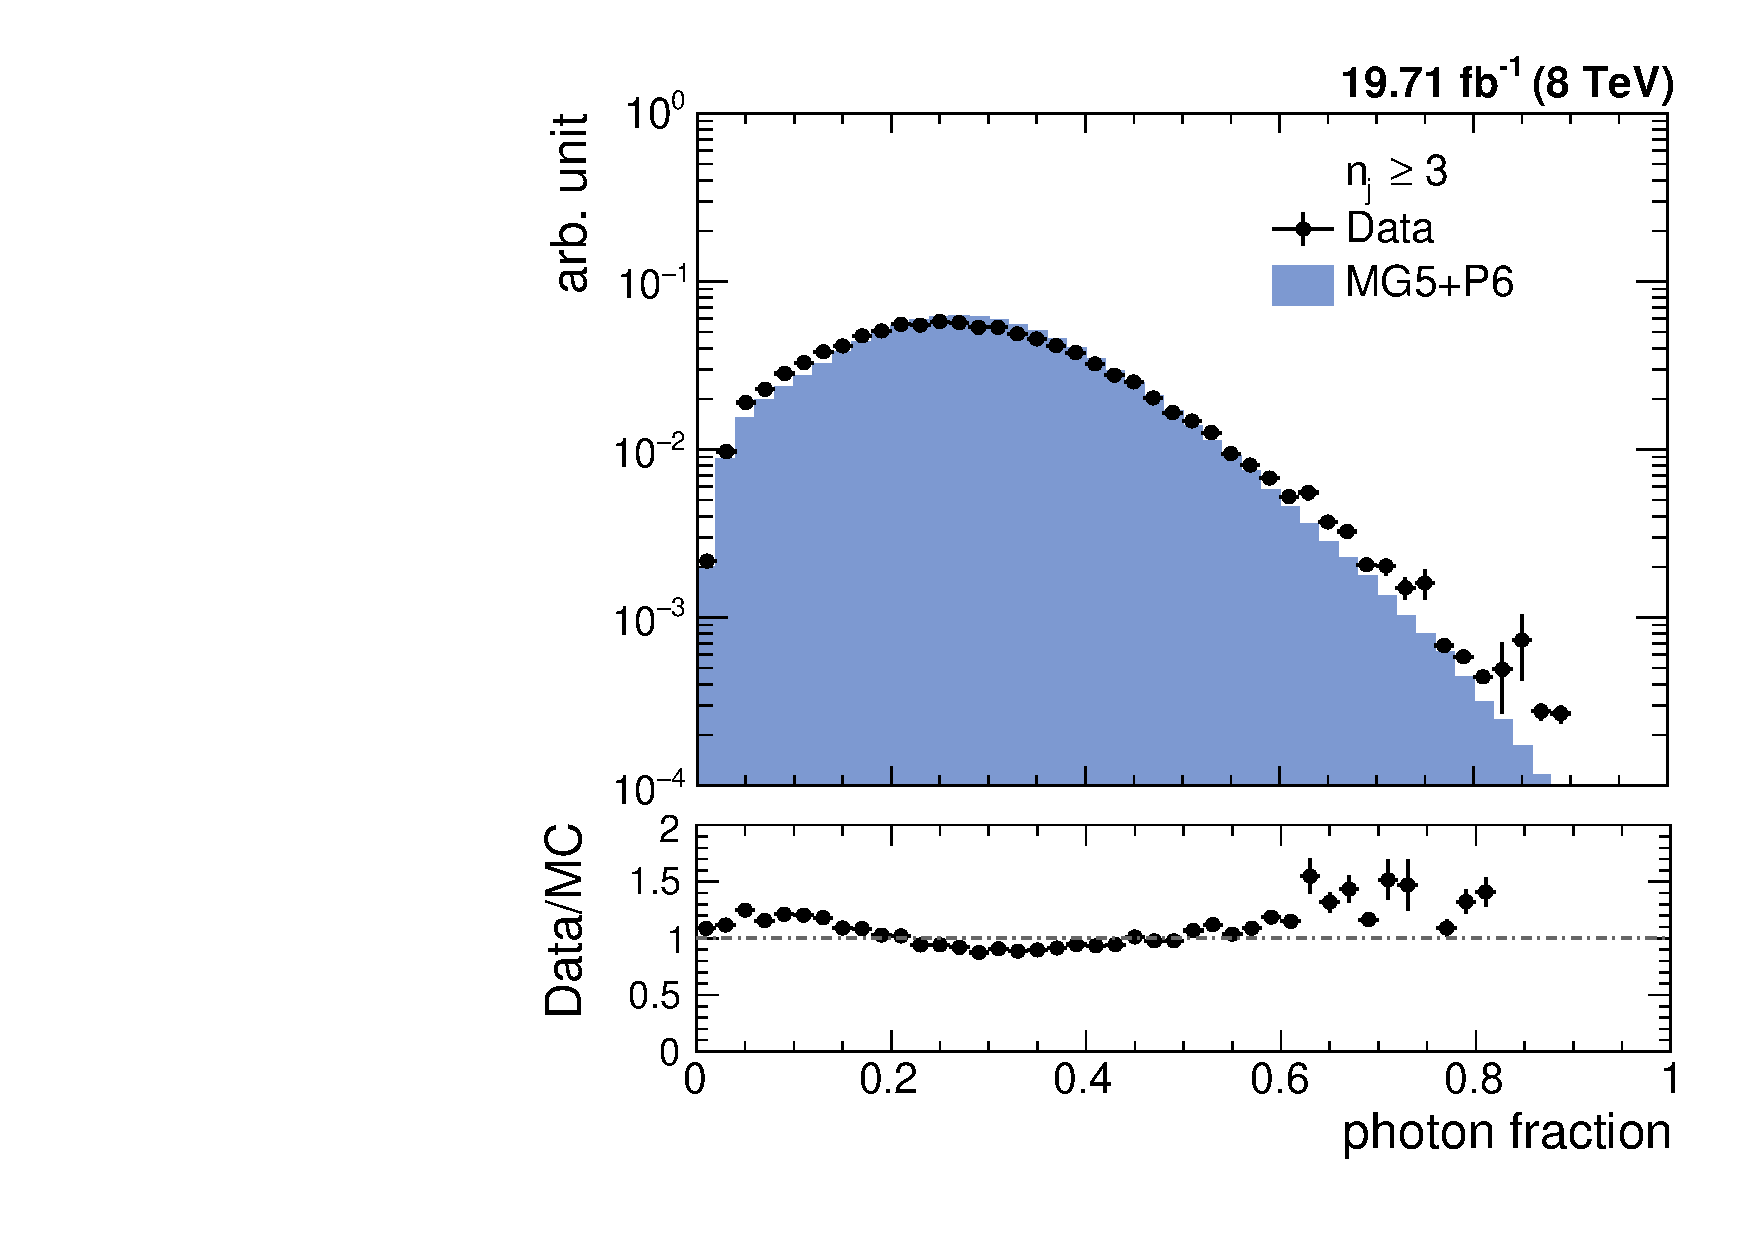
\includegraphics[width=0.51\textwidth]{Plots_HT_2_150/Comparison_PhFrac_3_HT_2_150.pdf}\\
 \vspace*{1mm}
 \hspace*{-2mm}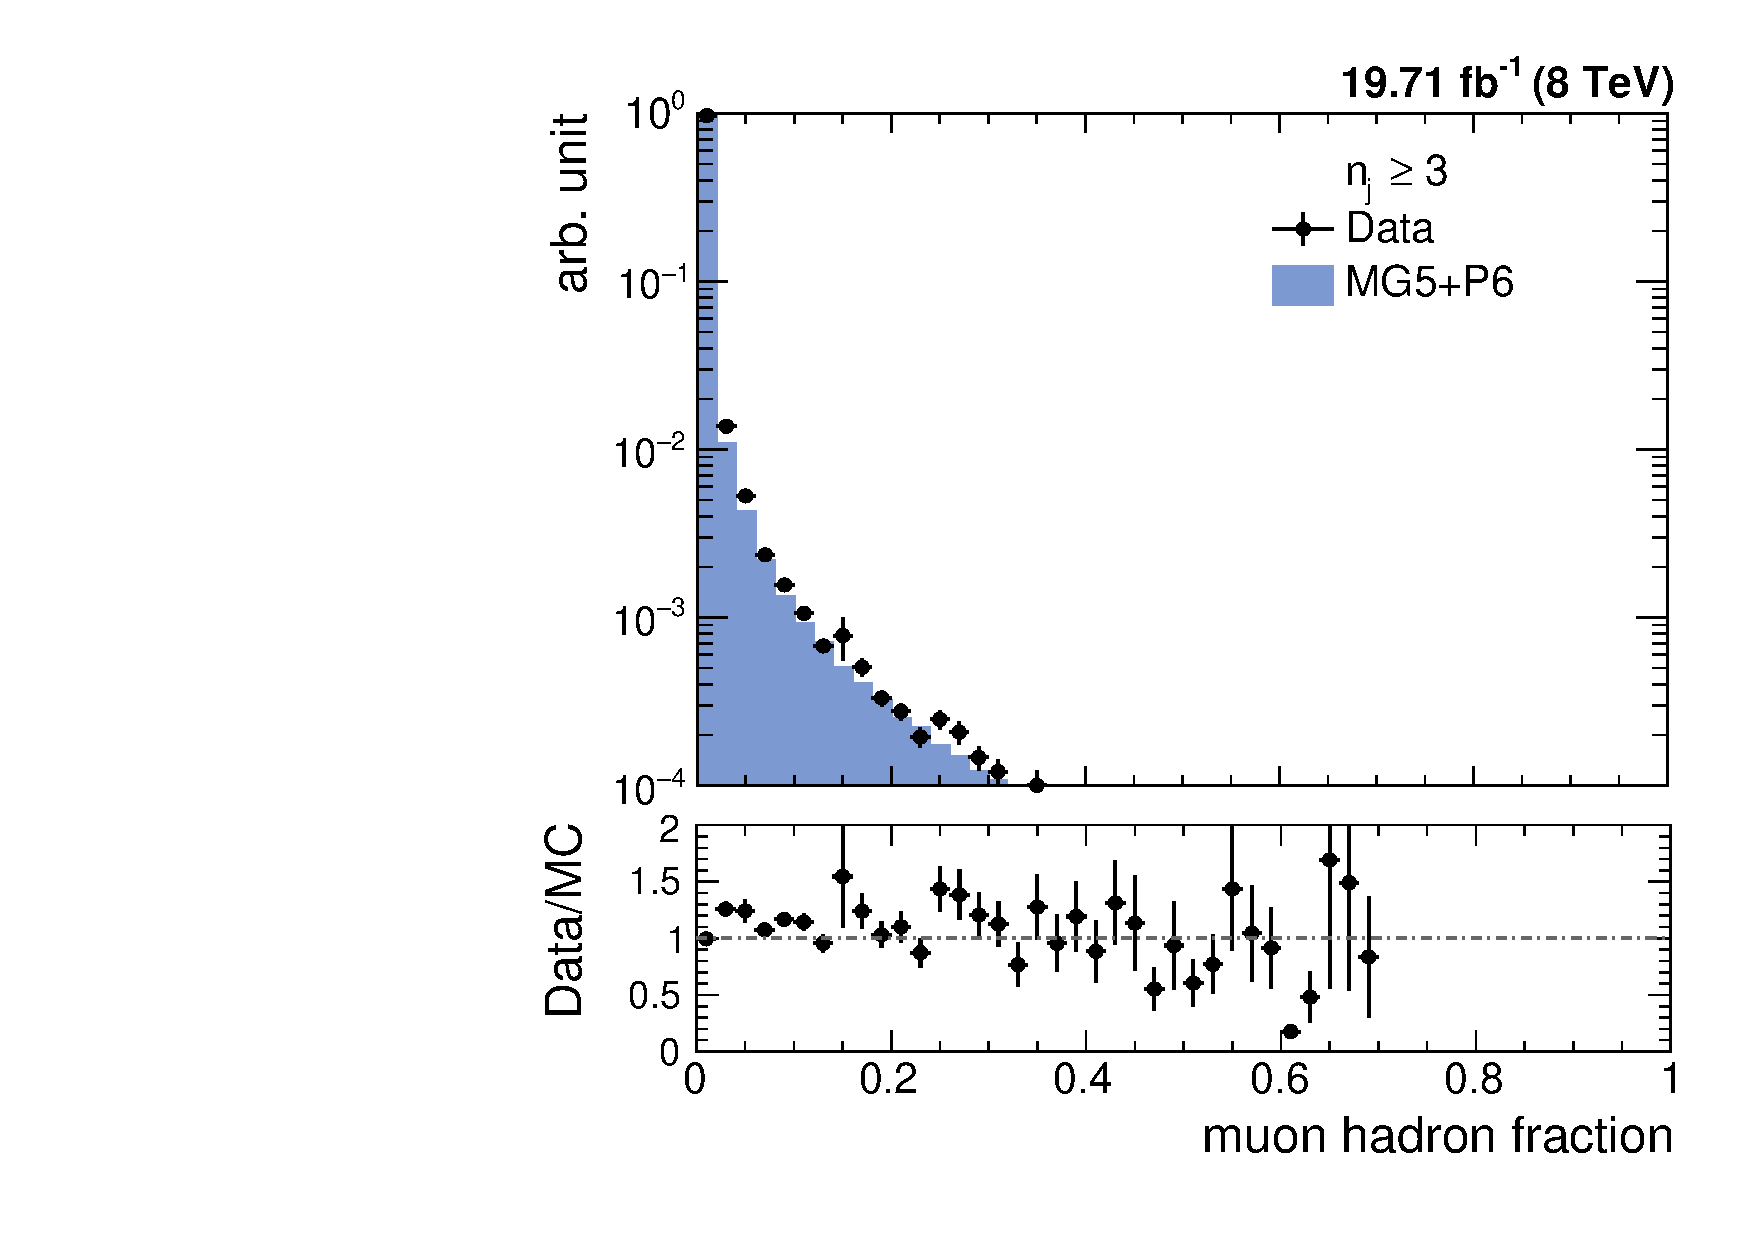
\includegraphics[width=0.51\textwidth]{Plots_HT_2_150/Comparison_MuFrac_3_HT_2_150.pdf}%
 ~~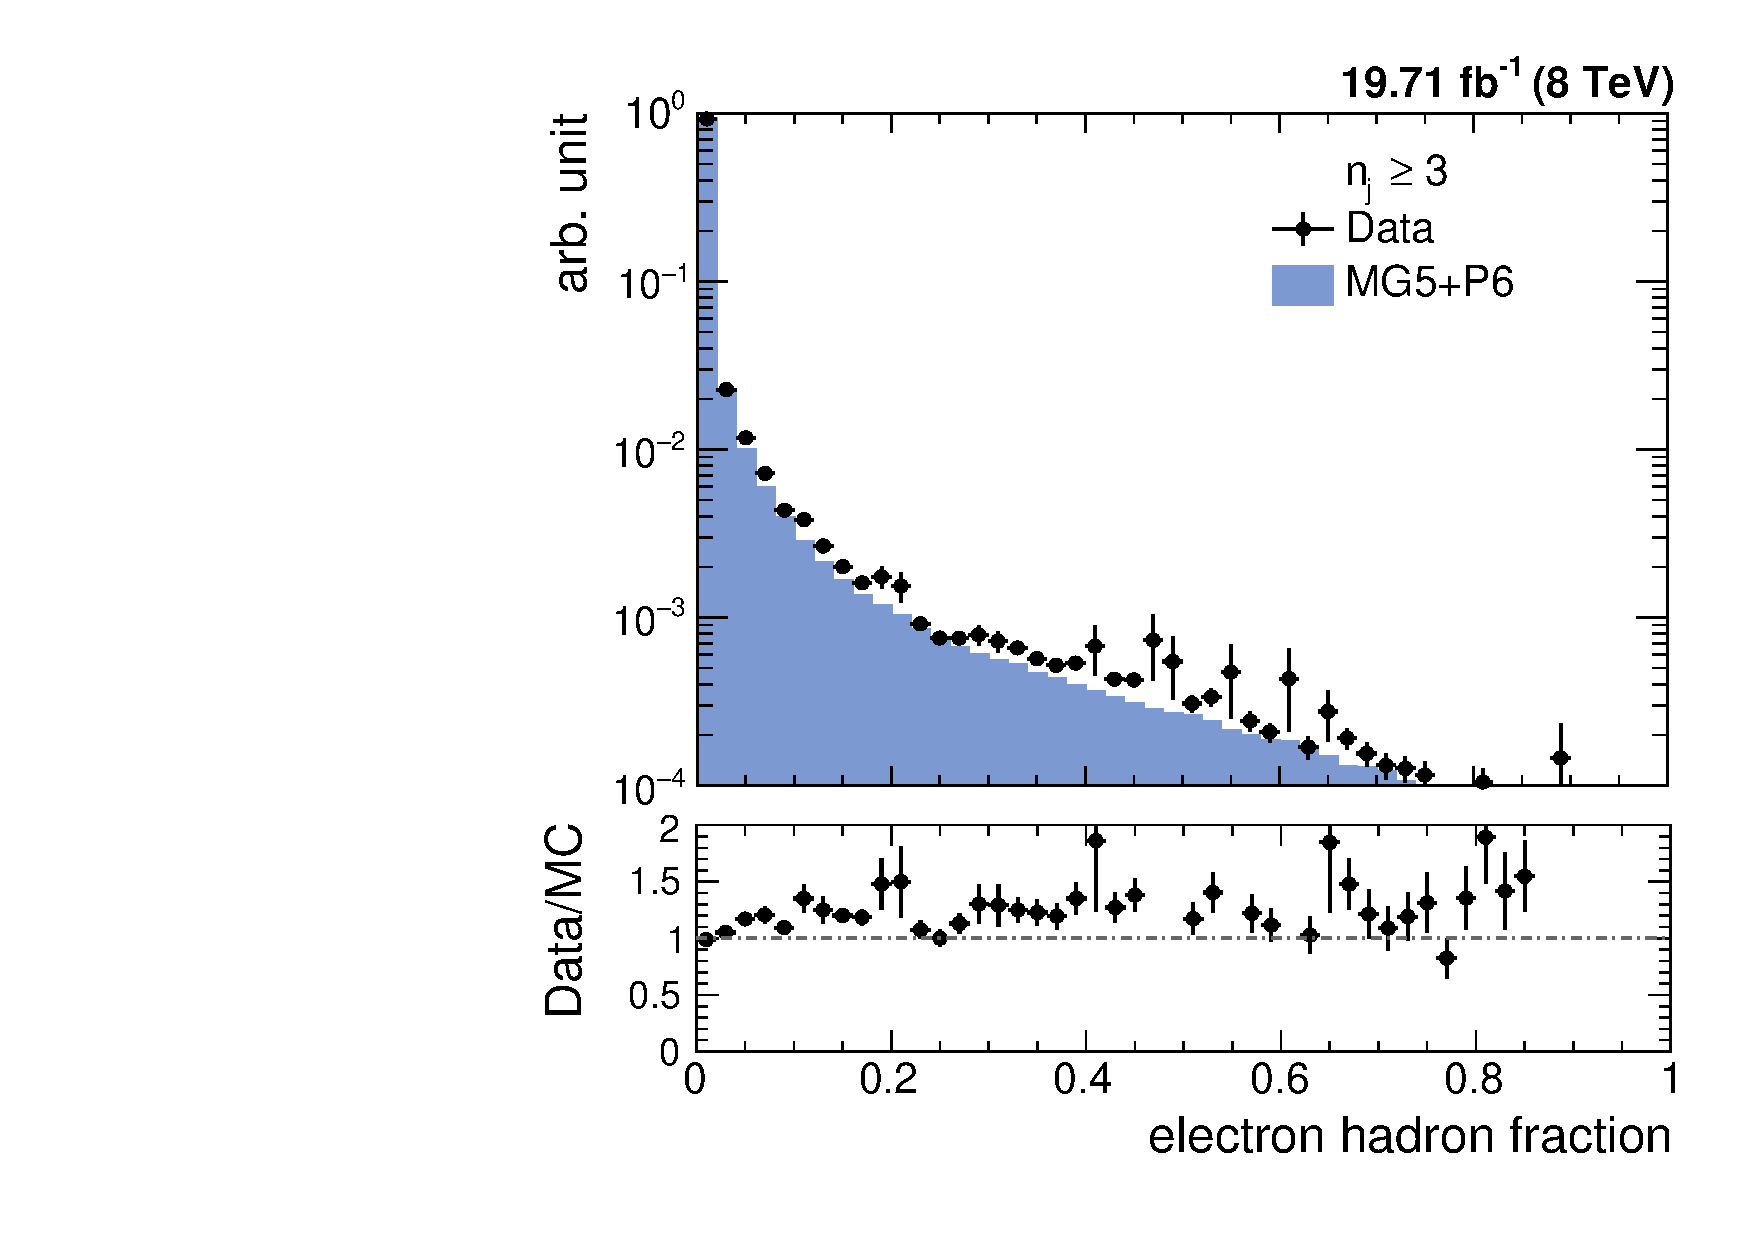
\includegraphics[width=0.51\textwidth]{Plots_HT_2_150/Comparison_ElFrac_3_HT_2_150.pdf}\\
 \vspace*{1mm}
 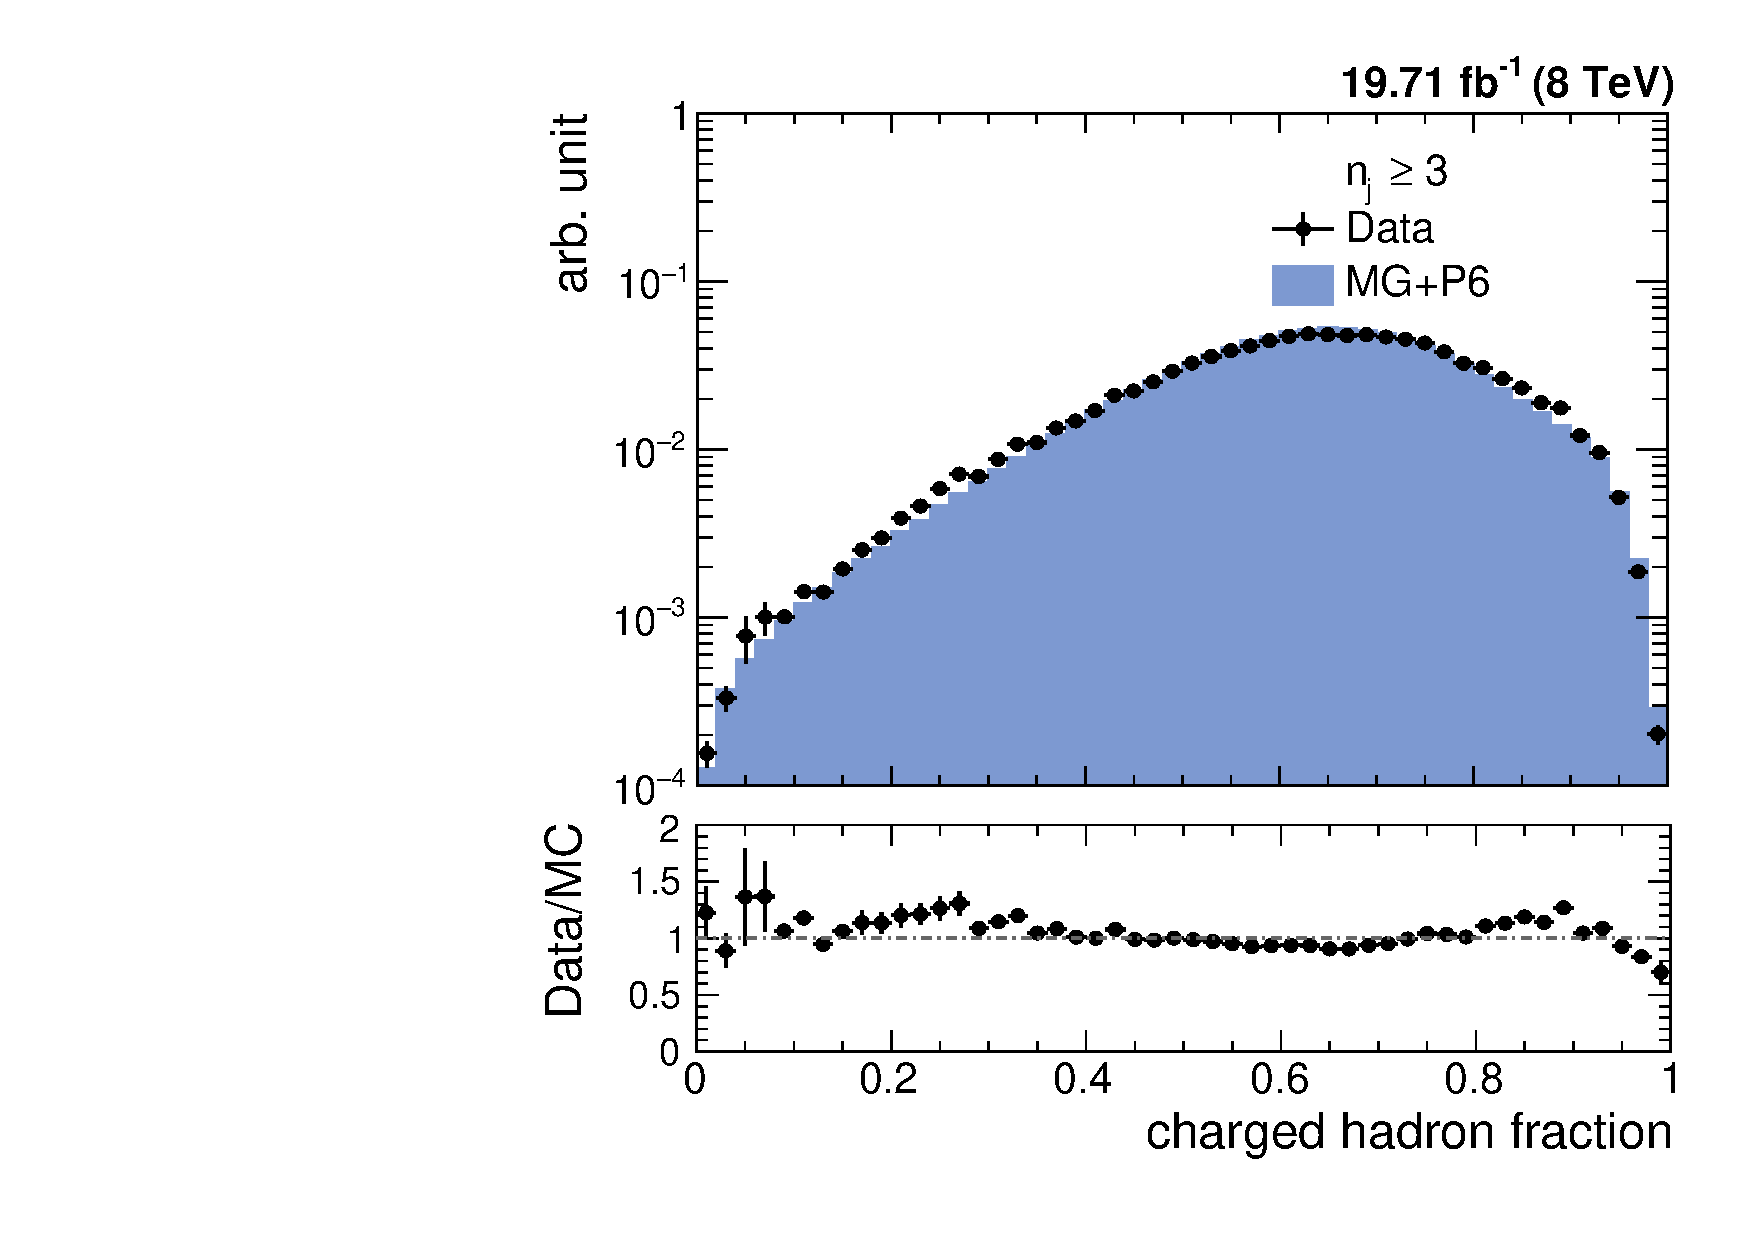
\includegraphics[width=0.51\textwidth]{Plots_HT_2_150/Comparison_ChHadFrac_3_HT_2_150.pdf}
 \caption[The fractions of jet constituents for different types of PF candidates for inclusive 3-jet events.]{The fractions of jet constituents as observed in data (black solid circles) and simulated Monte Carlo events (blue histogram) for different types of PF candidates for inclusive 3-jet events. Data and simulations are normalized to the same number of events. The distributions are shown after the application of the jet ID.}
 \label{fig:qual3}
 \end{center}
\end{figure} 

\subsubsection{Jet ID Efficiency}
The efficiency of the jet ID as a function of \httwo is studied using a tag-and-probe technique with dijet events. The two leading jets are required to be back-to-back in the azimuthal plane such that $|\Delta\phi - \pi|$ \ls 0.3. One of the dijets is selected randomly as a ``tag'' jet which is required to fulfill the tight jet ID criteria. The other jet is called ``probe'' jet for which it is examined, whether it also passes the tight jet ID. The ID efficiency is defined as the ratio of events where the probe jet passes the ID requirements, over the total number of dijet events. It is shown as function of \httwo in Fig.~\ref{fig:ideff} and as expected, it is always greater than 99\%. The QCD cross-section decreases as a function of \httwo and hence the number of events decrease on moving to higher \httwons. Consequently the statistical fluctuations for ID efficiency are larger at higher \httwons.

\begin{figure}[!htbp]
 \begin{center}
 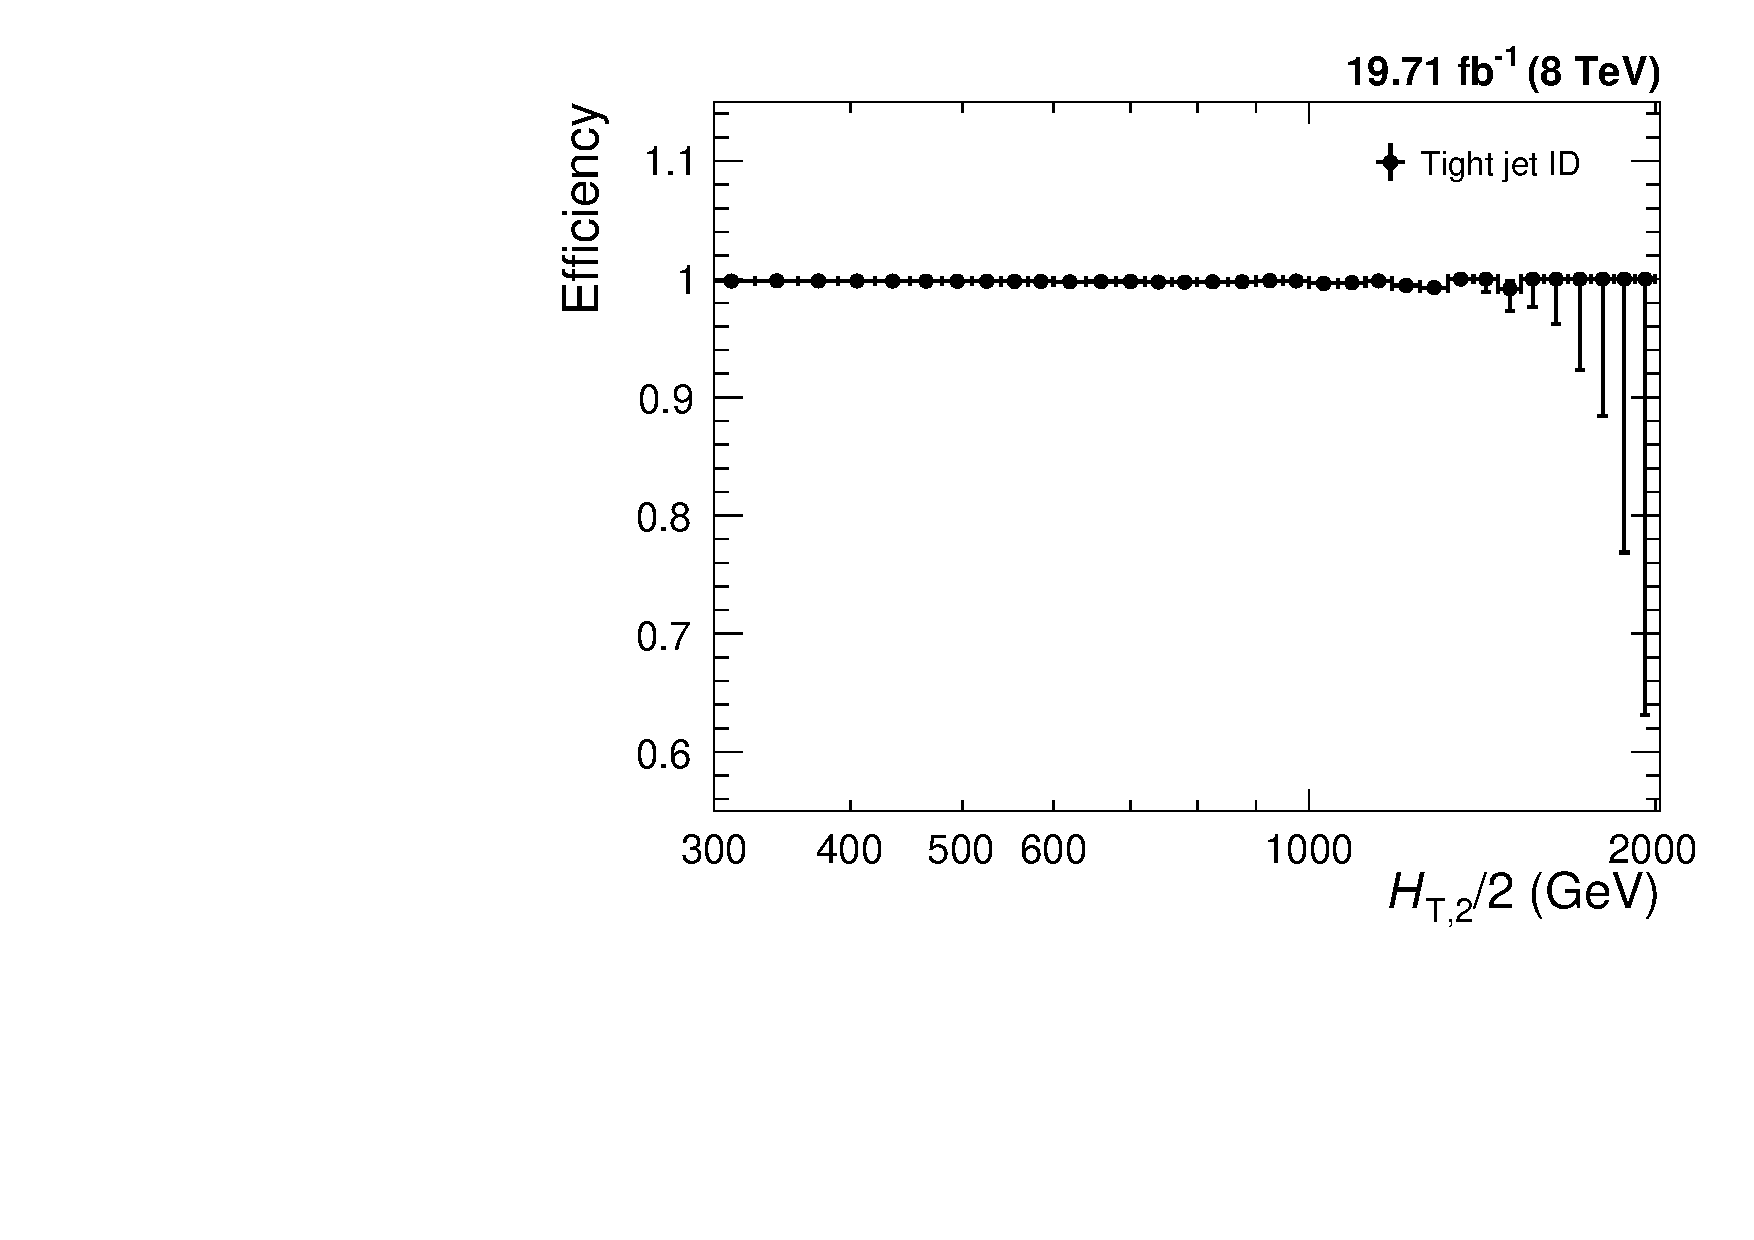
\includegraphics[width=0.53\textwidth]{/home/anter/Desktop/Thesis/Plots_HT_2_150/ID_Efficiency.pdf}
 \caption[The jet ID efficiency is studied as a function of \httwo with tag-and-probe technique using dijet event topologies and it always exceeds 99\%.]{The jet ID efficiency is studied as a function of \httwo with tag-and-probe technique using dijet event topologies and it always exceeds 99\%.}
 \label{fig:ideff}
 \end{center}
\end{figure} 

\subsection{Jet Selection}
The measurement of differential cross-sections and their ratio uses jets clustered from particle flow candidates using the anti-\kt jet algorithm with a size parameter, $R$ = 0.7. The energy scale of the jets is corrected with the CMS recommended jet energy corrections, described in Sec.~\ref{sec:jet_corrections}. These corrections are applied to jets in both data\footnote{Winter14\_V8 jet energy corrections} as well those in simulated events\footnote{START53\_V27 jet energy corrections}. As a convention, the jets in one event are in decreasing order of \pt, with the first (leading) jet being the jet with highest \pt. The jet selection, based on phase space cuts on transverse momentum and rapidity of jets in an event, is as follows : 

\begin{itemize}
\item All jets having \pt \gr 150 \GeV and $|y|$ \ls 5.0 are selected.
\item Events with at least two jets are selected.
\item The two leading jets should have $|y|$ \ls 2.5 and further jets are counted only, if they lie within the same central rapidity range of $|y|$ \ls 2.5. 
\end{itemize}

These cuts assure high detector acceptance and exactly same selection is applied in the measurement, simulated events as well in theoretical calculations for a consistent comparison. 

\section{Comparison with Simulation}
\subsection{Pileup Reweighting}
While generating the official Monte-Carlo samples, the number of pileup interactions describing the conditions expected for each data-taking period are taken care of. But the number of pileup events implemented in the simulation $N_{\rm MC} (N_{\rm PU,truth})$, does not match exactly with the one measured actually in data $N_{\rm data} (N_{\rm PU,est.})$. To match the pileup distributions in data, a reweighting factor $w_{\rm PU}$, as given by Eq.~\ref{eq:reweigh} is applied to the simulated events. In Fig.~\ref{fig:pileup} the number of reconstructed vertices are shown before (left) and after pileup reweighting (right). It is observed that before pileup reweighting there was a significant mismatch of the pileup distributions in data (black solid circles) and simulated MC events (blue histogram), which completely vanishes after reweighting. 

\begin{equation}
\label{eq:reweigh}
 {w_{\rm PU} = \frac {N_{\rm data} (N_{\rm PU,est.})/\sum N_{\rm data}} {N_{\rm MC} (N_{\rm PU,truth)}/\sum N_{\rm MC}}}
\end{equation}

\begin{figure}[ht]
 \begin{center}
 \hspace*{-5mm}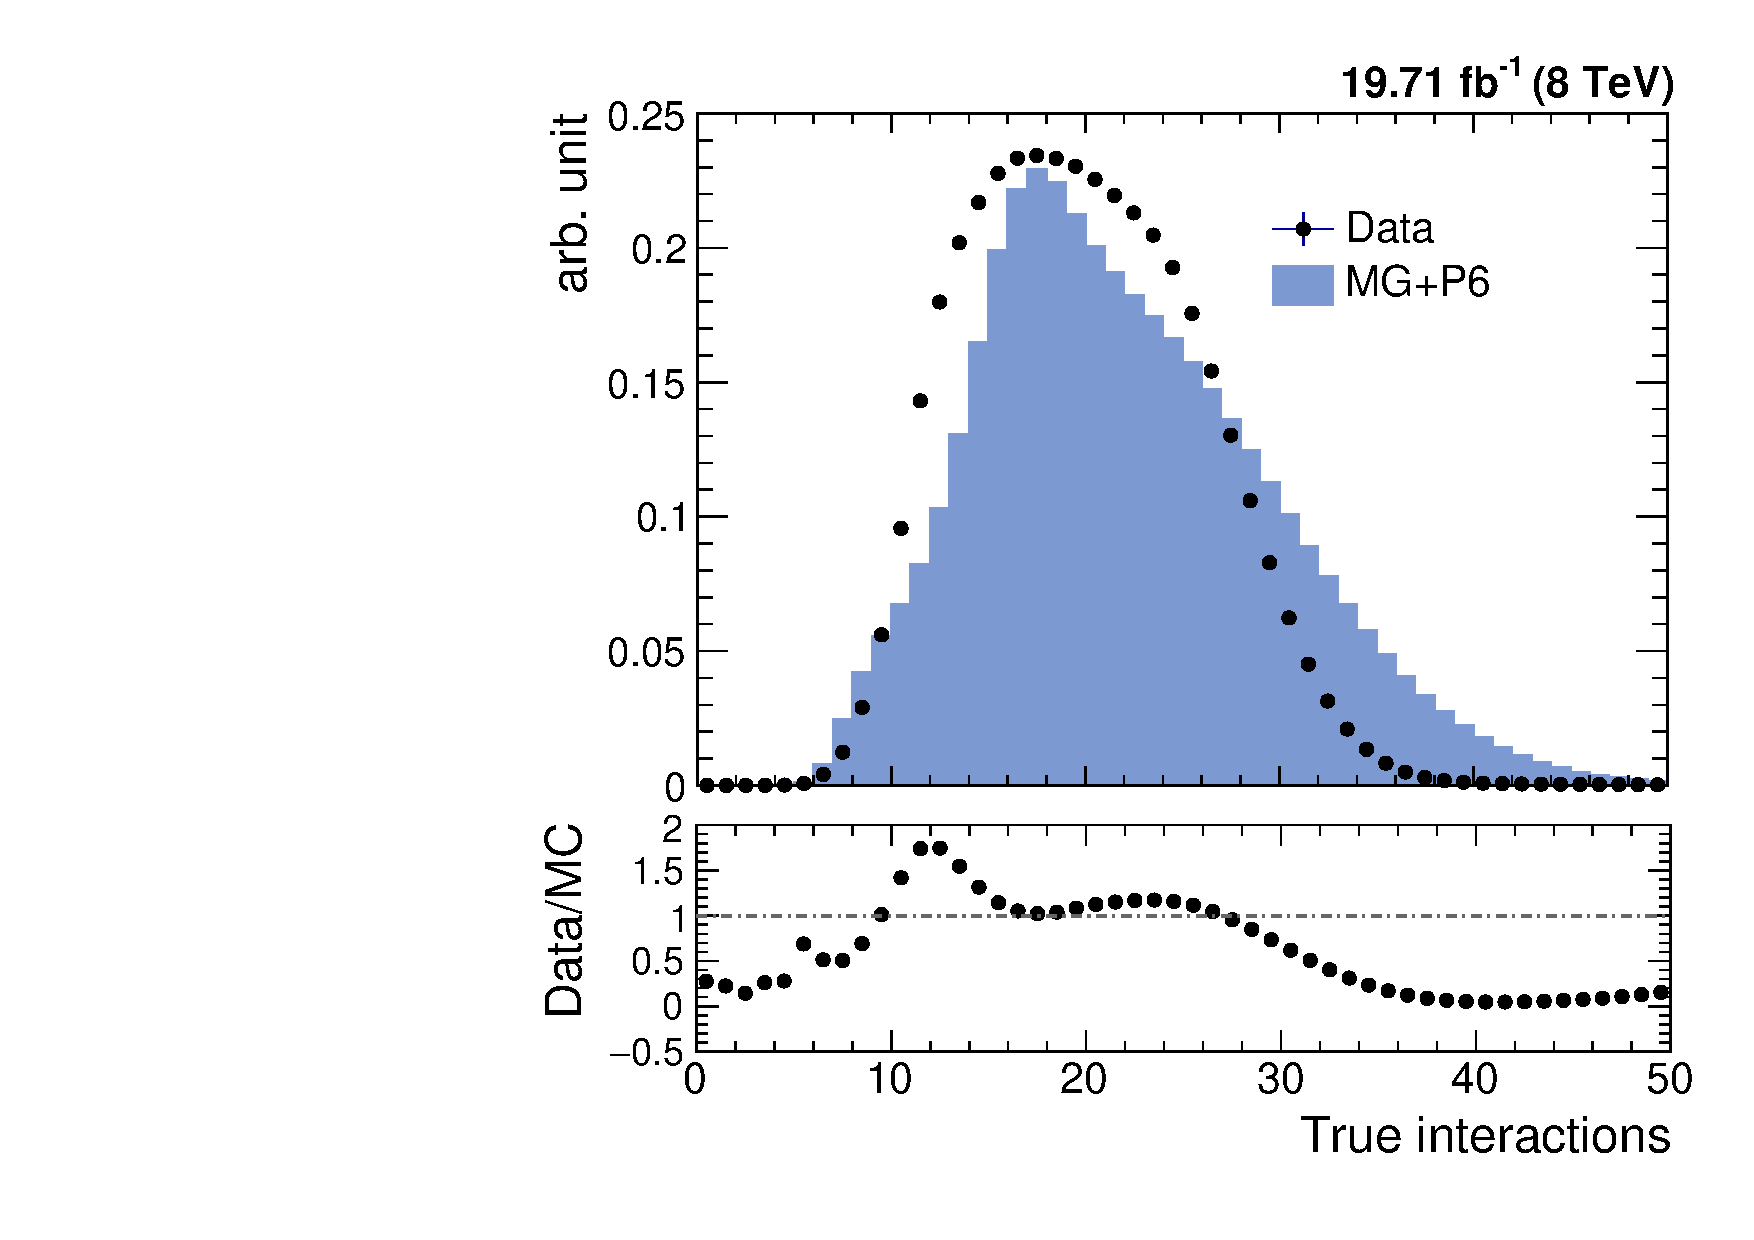
\includegraphics[width=0.51\textwidth]{Plots_HT_2_150/Nvertices.pdf}%
 ~~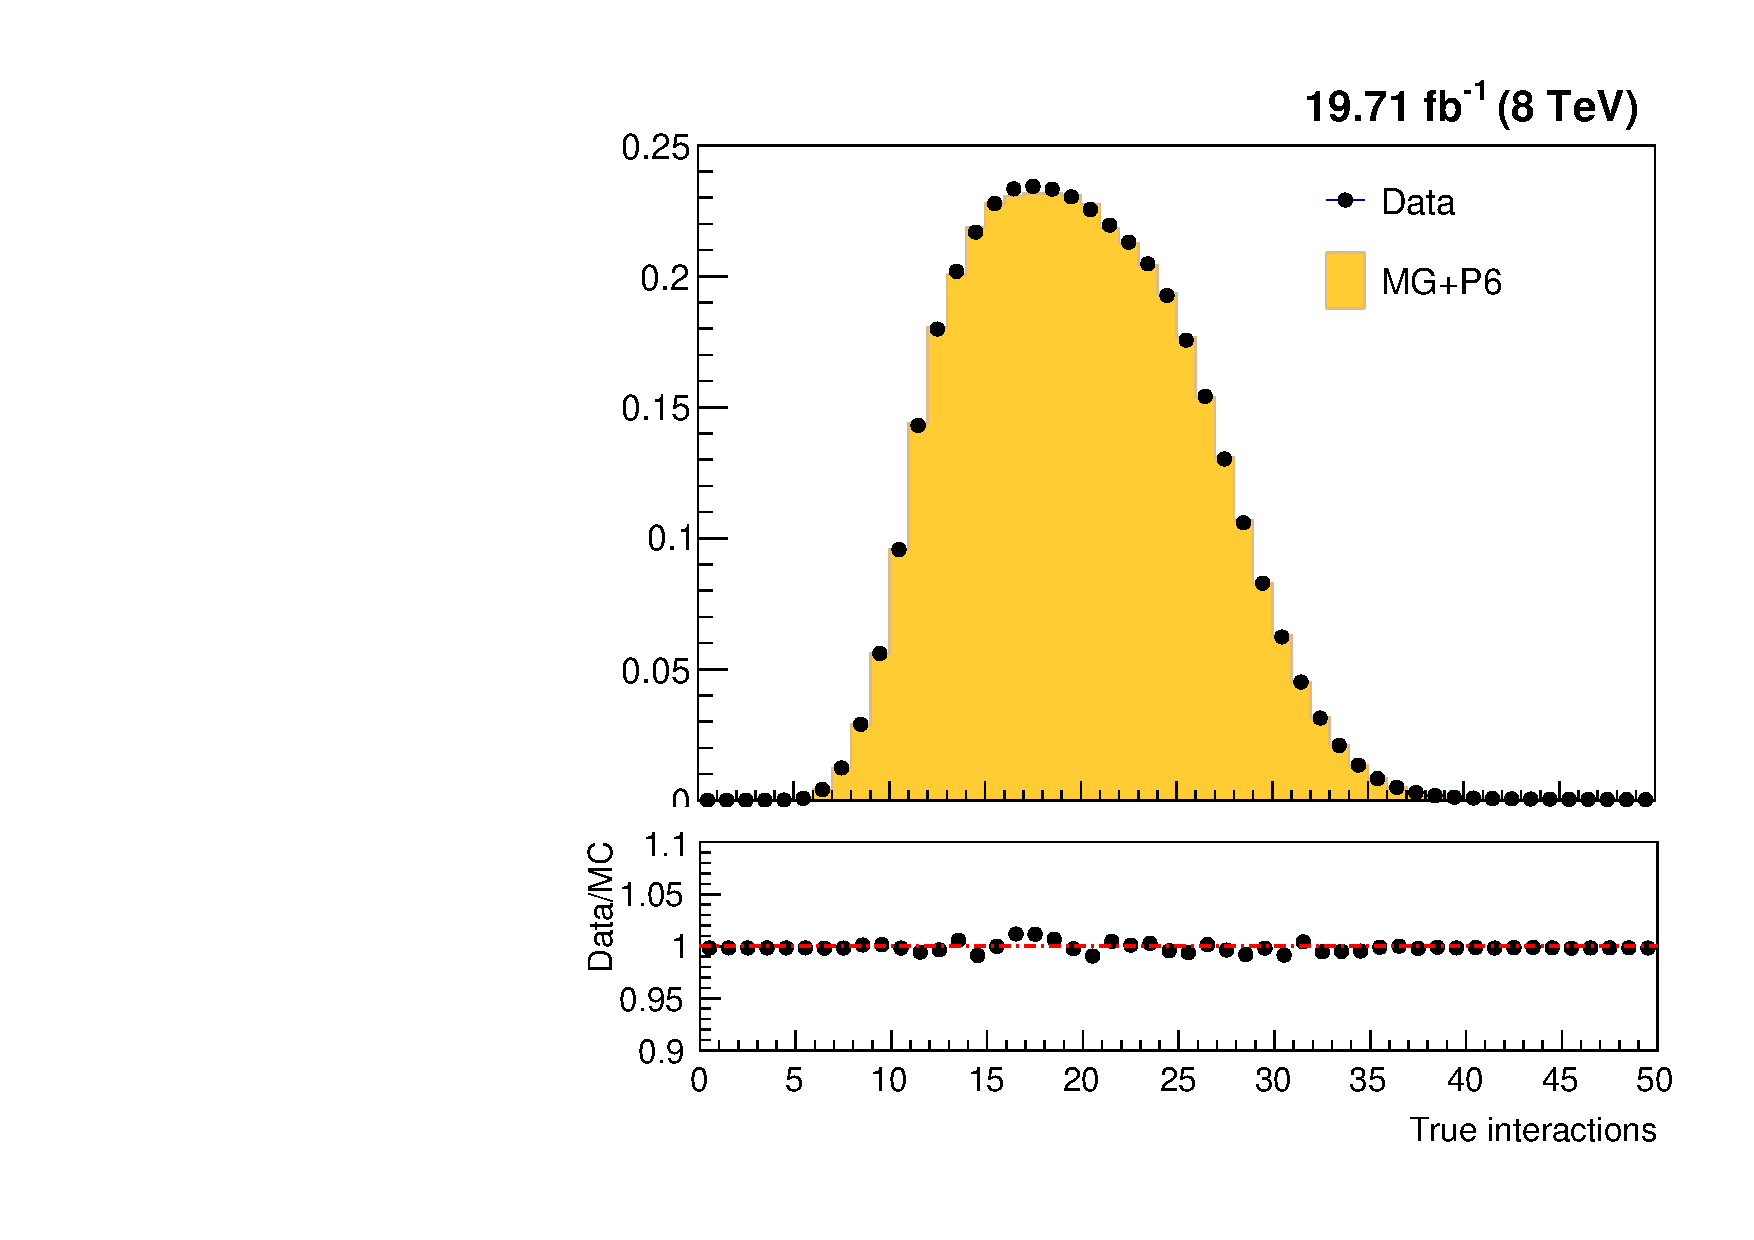
\includegraphics[width=0.51\textwidth]{Plots_HT_2_150/Nvertices_weight.pdf}
 \caption[Number of reconstructed vertices before and after the pileup reweighting.]{Number of reconstructed vertices in data (black solid circles) and simulated Monte Carlo events (blue histogram) before (left) and after (right) the pileup reweighting.}
 \label{fig:pileup}
 \end{center}
\end{figure}

\subsection{Comparison of Cross-sections and their Ratio}
The measured data distribution of differential cross-section at detector level is compared to the predictions of Monte Carlo simulation using \MadGraphF generator interfaced with \PYTHIAS (\MGP) including the detector simulation as well as to a fixed-order theory prediction obtained using CT10-NLO PDF set. Figure~\ref{fig:comp_all} shows the comparison of differential cross-section as a function of \httwo for \njt~(left) and \njth~events (right), for data (black solid circles), \MGP~MC (red empty circles) and CT10-NLO (blue histogram). The bottom panel in each plot shows the ratio of data to the MC predictions (red line) as well as to the CT10-NLO theory predictions (blue line). The NLO predictions on parton level are not corrected for non-perturbative effects. Still the NLO predictions describe the data better as compared to the LO MC simulations which roughly describes the spectrum on detector level. The sufficient data for \njt~and \njth~events are available up to \httwo = 2000 GeV and 1680 GeV, respectively. Due to some kinematical constraints, the minimum cut on \httwo is 300 GeV (explained in Sec.~\ref{sec:nlo_factors}). Hence the differential cross-sections are studied in the range 300 GeV $\leq$ \httwo \ls 2000 GeV for \njt~and 300 GeV $\leq$ \httwo \ls 1680 GeV for \njth~events.

\begin{figure}[!htbp]
 \begin{center}
 \hspace*{-5mm}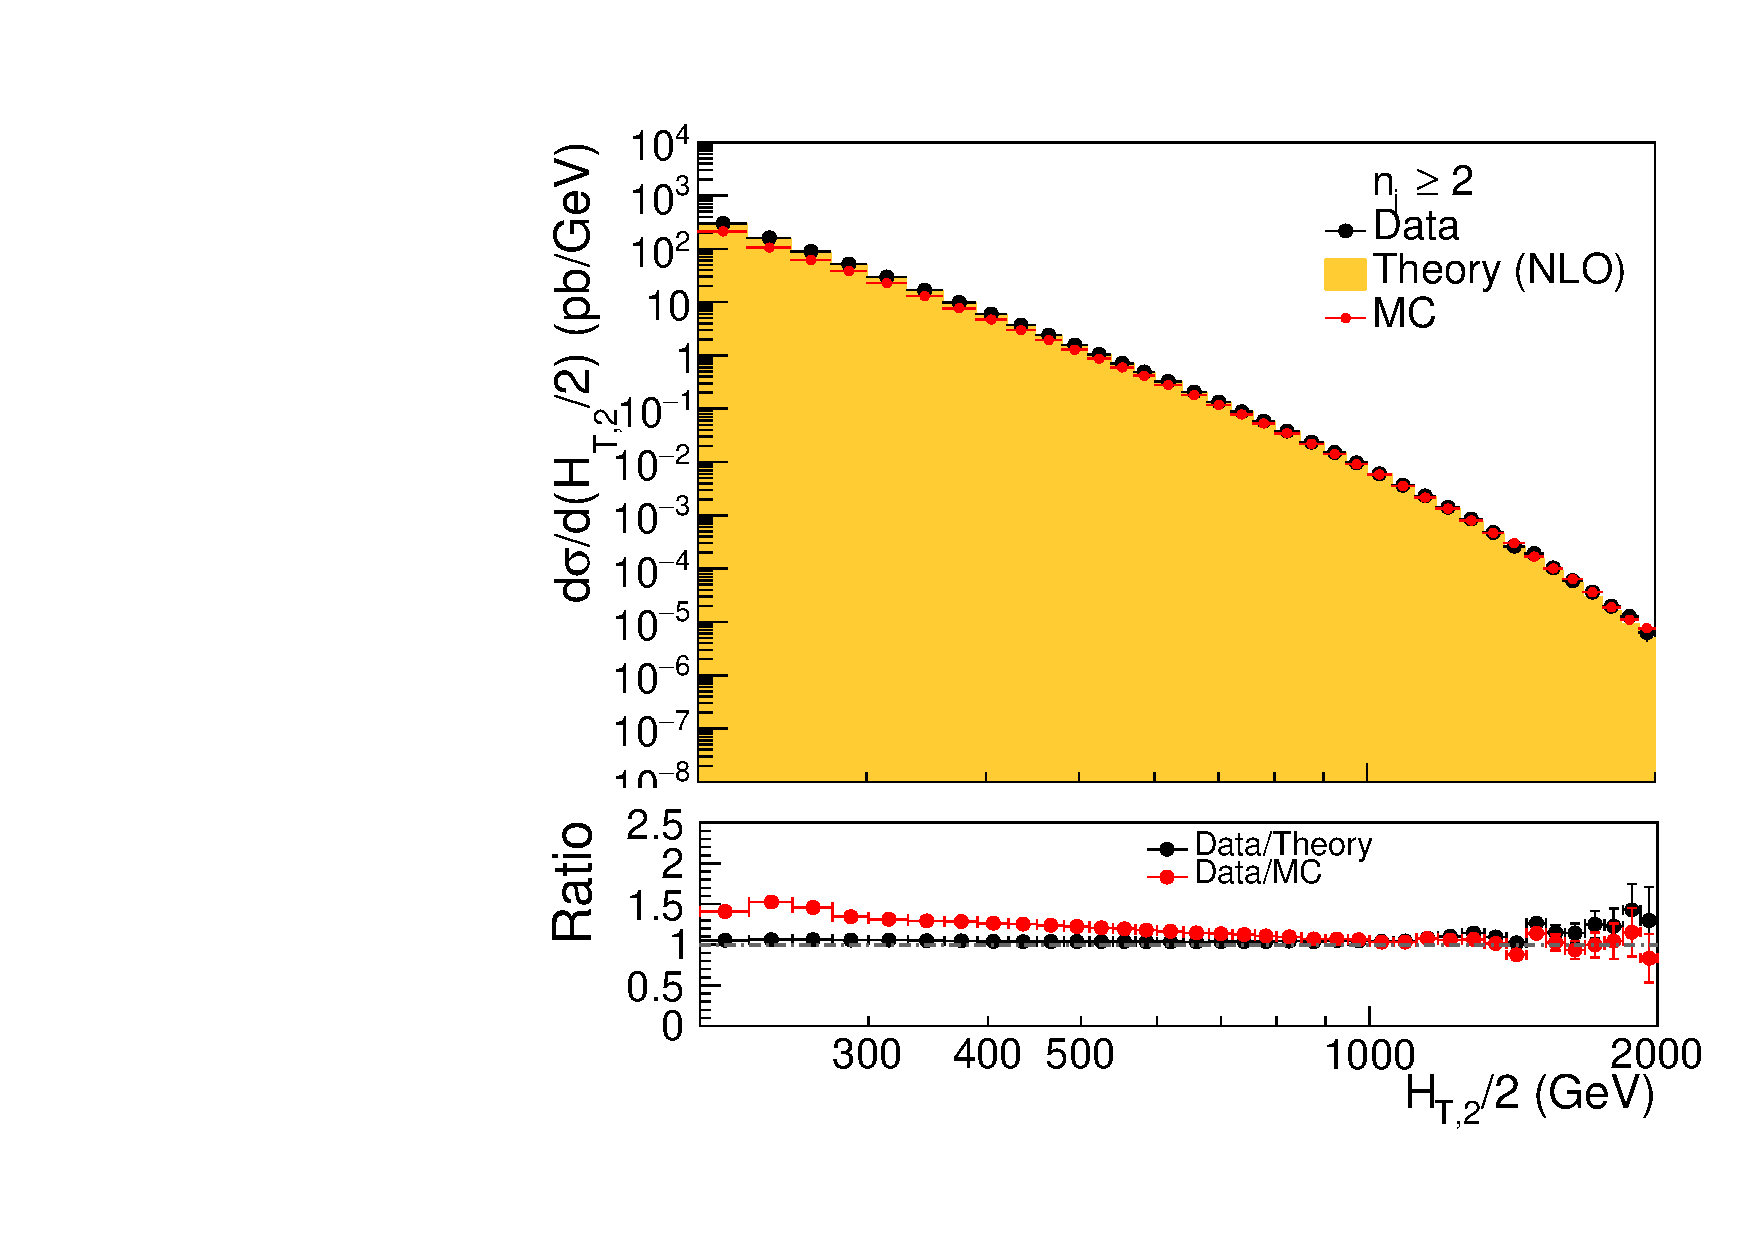
\includegraphics[width=0.51\textwidth]{Plots_HT_2_150/Comparison_all_2_HT_2_150.pdf}%
 ~~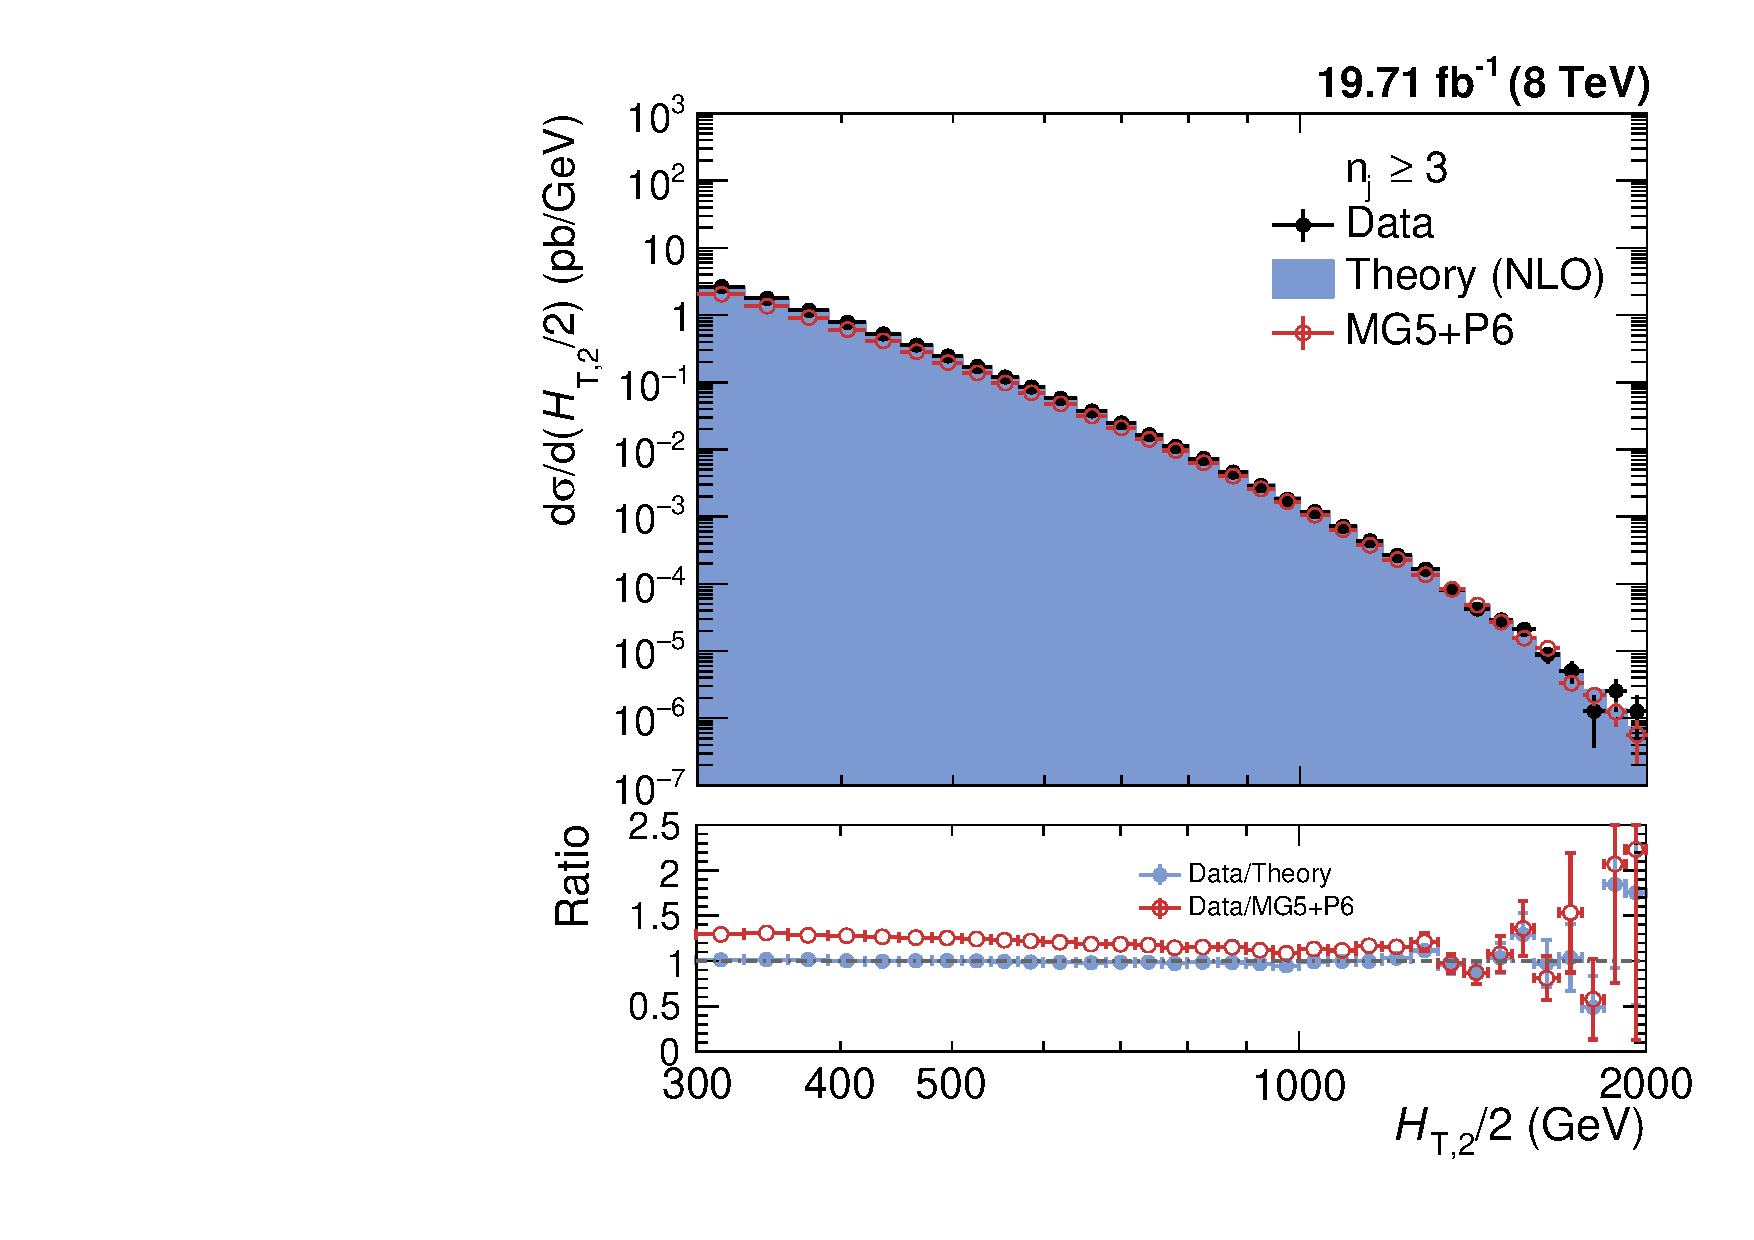
\includegraphics[width=0.51\textwidth]{Plots_HT_2_150/Comparison_all_3_HT_2_150.pdf}
 \caption[Comparison of differential cross-sections for data with simulated events and CT10-NLO theory predictions.]{The reconstructed level differential cross-sections are compared for data (black solid circles) and LO \MadGraphFn\plusn \PYTHIAS (\MGP) Monte Carlo (red empty circles) simulations with CT10-NLO theory predictions (blue histogram), as a function of \httwo for inclusive 2-jet (left) and 3-jet events (right). Ratios of data to the Monte Carlo predictions (red line) as well as to the CT10-NLO predictions (blue line) are shown in bottom panel of each plot.}
 \label{fig:comp_all}
 \end{center}
\end{figure}

\begin{figure}[!h] 
 \begin{center}
 \hspace*{-5mm}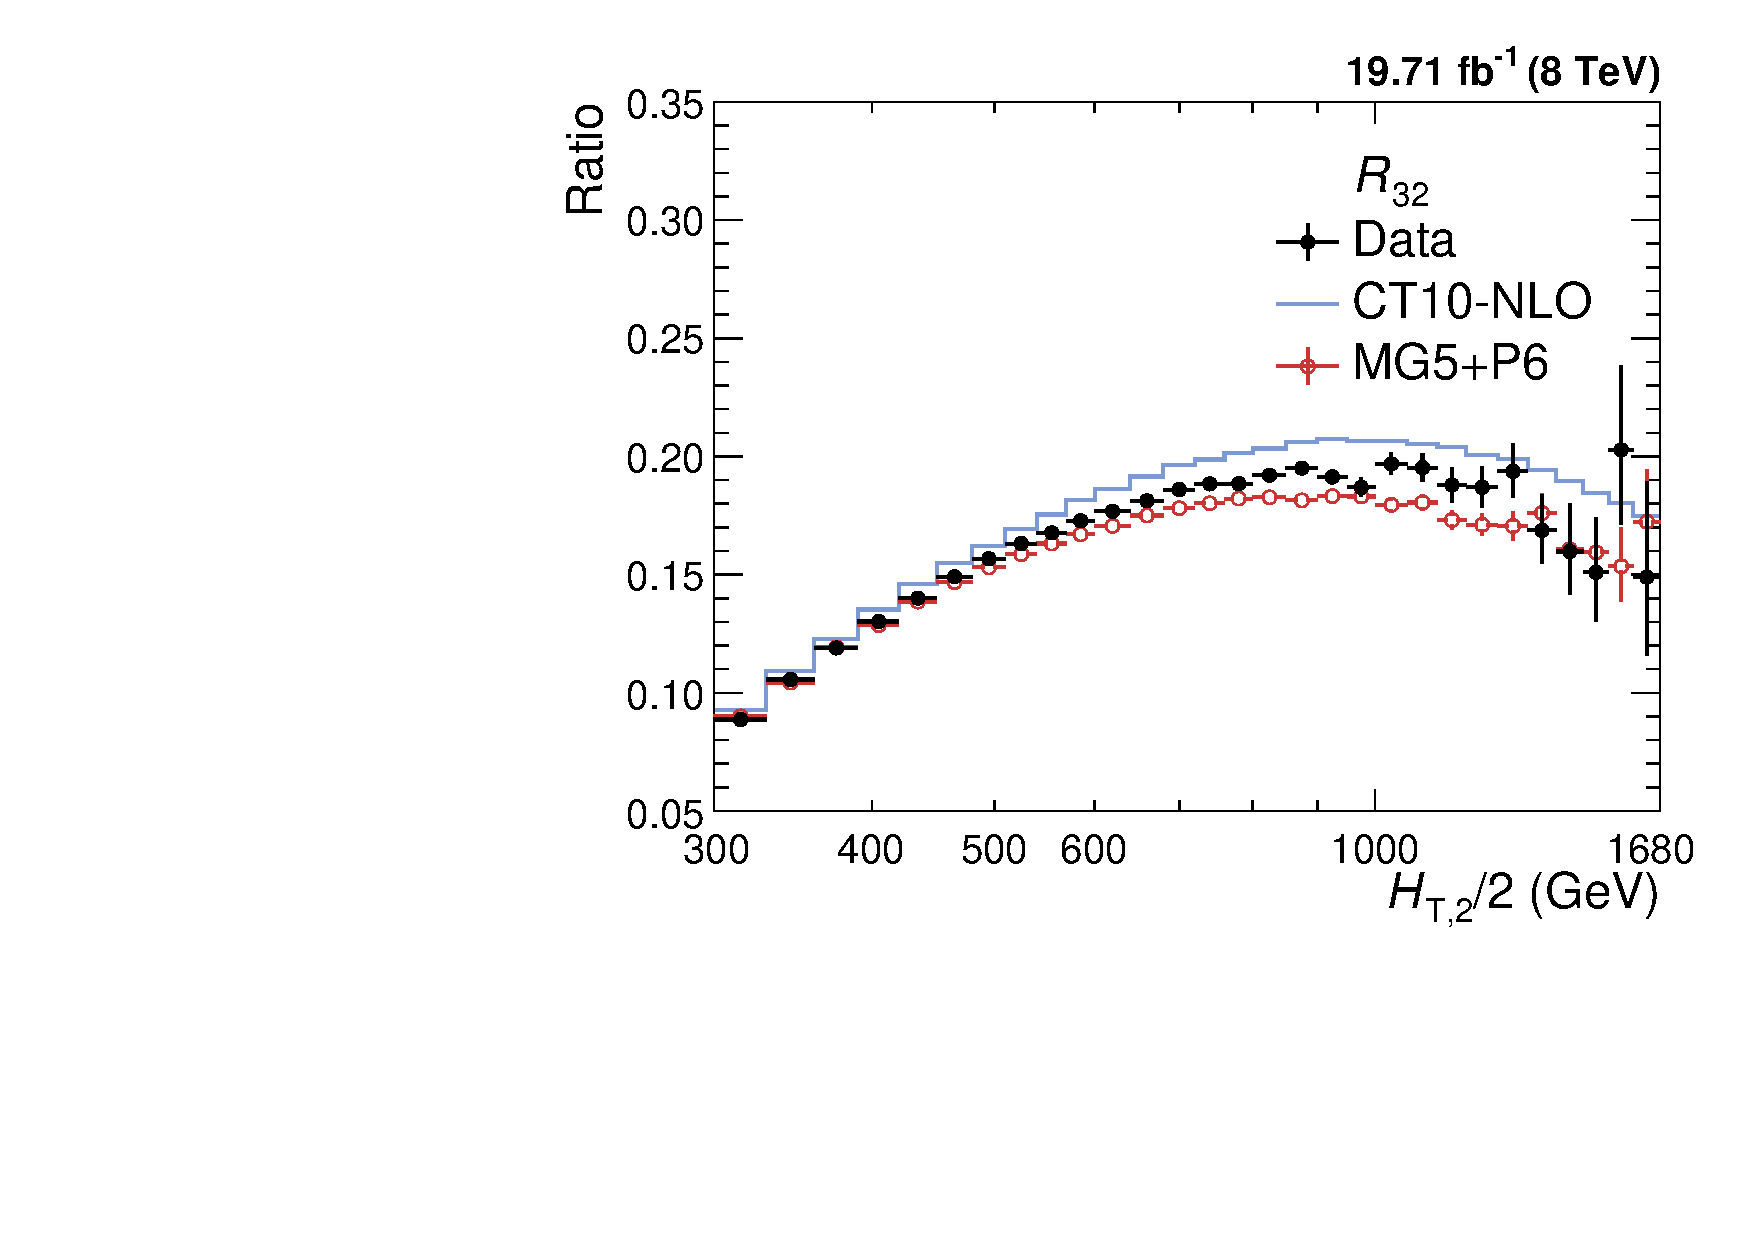
\includegraphics[width=0.5\textwidth]{Plots_HT_2_150/Ratio_32_all_HT_2_150.pdf}
 \caption[Comparison of the cross-section ratio for data with simulated events and CT10-NLO theory predictions.]{Comparison of the reconstructed level cross-section ratio \ratio as a function of \httwons, for data (black solid circles) and LO \MadGraphFn\plusn \PYTHIAS (\MGP) Monte Carlo (red empty circles) with CT10-NLO theory predictions (blue line). The error bars give the asymmetrical statistical uncertainty, calculated by the Wilson score interval method which takes into the account the correlation between the numerator and denominator.}
 \label{fig:ratio_32}
 \end{center}
\end{figure}

The ratio of differential cross-sections, $R_{32}$ as a function of $\httwo$, is extracted by dividing the cross-section of selected inclusive 3-jet events to that of inclusive 2-jet events at any given bin size of \httwo. In the cross-section ratios, the numerator and denominator are not independent samples. So to calculate the statistical uncertainty for the cross-section ratios at reconstructed level, the Wilson score interval method is used which takes into account the correlation between the numerator and the denominator and give asymmetric errors. Figure~\ref{fig:ratio_32} shows the comparison of the cross-section ratio \ratio as a function of \httwons, for data (black solid circles) and LO \MadGraphFn\plusn \PYTHIAS (\MGP) Monte Carlo (red empty circles), at reconstructed level with CT10-NLO theory predictions (blue line). Since in \njth~events, the enough statistics for differential cross-section is available up to 1680 GeV of \httwo only, \ratio is also studied in the range 300 GeV $\leq$ \httwo \ls 1680 GeV. The bin-wise inclusive 2-jet and 3-jet events differential cross-sections as well as their ratio \rations, calculated at detector level, along with statistical uncertainty (in \%) are tabulated in Table~\ref{tab:ratio_32}. 

\section{Jet Energy Resolution (JER)}
\label{sec:Resolution}
In an ideal experiment, the value of a physical quantity would be determined exactly with an infinite precision. For e.g. whenever a particle with energy E passes an ideal calorimeter having infinite resolution, the measured energy should always be equal to E. But in real world, the measured energy of the above mentioned particle might differ from the value E. This difference of the measured quantity from its true value may be due to detector noise, uncertainties in the calibration, non-linearity of the response etc. Hence this results in the finite value of the resolution of the detector known as jet energy resolution (JER). In such case, the measured values of energy of different particles, passing through the same detector with same energy E, will be different. Such measurements are described by a Gaussian distribution which is centered around the true value of the measured quantity and its width is generally interpreted as detector resolution. Hence the importance of the detector resolution lies in the fact that it indicates how much the measured value of the observable differs from the true one i.e. how precisely a physical observable can be measured. The narrower the distribution, the higher the resolution is and hence the more efficient is the detector. %The measurement of detector resolution helps in the determination of the histogram binning of the observable to be studied. In binned histograms, it is possible that the measured quantity may migrate from one bin to another with respect to their true value. To avoid these migrations, the bin width should be at least two-three times larger than the detector resolution in that particular bin. The bin widths may also differ between each other for the same observable.

Due to finite resolution of the CMS detector, the measured transverse momentum of jets gets smeared. Since the observable in this study i.e. \httwo is the average sum of transverse momentum of leading and sub-leading jets, the resolution of the detector has to be studied in terms of the observable. CMS detector simulation based on \MGP~MC event generators is used to determine the resolution as both the particle and reconstructed level information is available. The jets clustered from stable generator particles called Gen jets as well as from particle flow candidates reconstructed from the simulated detector output called Reco jets, are used. The studies of the \JetMet working group at CMS has shown that the jet energy resolution in data is actually worse than in simulation \cite{JER}. So the reconstructed jet transverse momentum needs to be smeared additionally to match the resolution in data. Table~\ref{tab:resolution} shows the scaling factors (c) which need to be applied on the transverse momentum of simulated reconstructed jets. The scaling factors depend on the absolute $\eta$ of the jet. The uncertainty on these measured scaling factors (c$_{central}$) needs to be taken into account in a physics analysis. This is done by smearing the reconstructed jets with two additional sets of scaling factors, c$_{up}$ and c$_{down}$, that correspond to varying the factors up and down respectively, by one sigma and evaluating the impact of these new sets. 

\begin{table}[!htbp]
\centering
 \caption[The jet energy resolution in data is actually worse than in simulation. To match the resolution in data, the reconstructed jet transverse momentum in simulated events need to be smeared by applying the scale factors.]{\JetMet working group at CMS has shown that the jet energy resolution in data is actually worse than in simulation \cite{JER}. To match the resolution in data, the reconstructed jet transverse momentum in simulated events need to be smeared by applying the scale factors. The uncertainty on the resolution is given by an upwards and downwards variation c$_{up}$ and c$_{down}$ of the measured scaling factor c$_{central}$.}
 \label{tab:resolution}
 \vspace{2mm}
 \begin{tabular}{lccccc}
  \hline\hline
    $~~~\eta$  & $0.0$ - $0.5$ & $0.5$ - $1.1$ & $1.1$ - $1.7$ & $1.7$ - $2.3$ & $2.3$ - $2.8$  \rbthm\\ \hline

    c$_{central}$    & 1.079   & 1.099   & 1.121    & 1.208   & 1.254    \rbtrr\\
    c$_{down}$       & 1.053   & 1.071   & 1.092    & 1.162   & 1.192    \rbtrr\\
    c$_{up}$         & 1.105   & 1.127   & 1.150    & 1.254   & 1.316    \rbtrr\\ 
    \hline\hline
  \end{tabular}
\end{table}

The reconstructed jet \pt is smeared randomly using a Gaussian width widened by the scaling factor (c$_{central}$) 
\begin{equation}
\pt \rightarrow Gauss\bigg(\mu = \pt, \sigma = \sqrt{c^2_{central} - 1} \cdot {\rm JER}(\pt)\bigg)
\end{equation}
where JER(\pt) is the resolution determined as a function of jet \pt using \MGP~MC simulated events. After smearing transverse momentum of each reco jet, \httwo is calculated from both generator particle jets (Gen \httwons) as well as the particle flow or reconstructed jets (Reco \httwons). Then the response is calculated as defined in the Eq.~\ref{eq:res}. 
\begin{equation}
\label{eq:res}
  R = \frac{{\rm Reco}~\httwo}{{\rm Gen}~\httwo}
\end{equation}

\begin{figure}[ht]
 \begin{center}
 \hspace*{-5mm}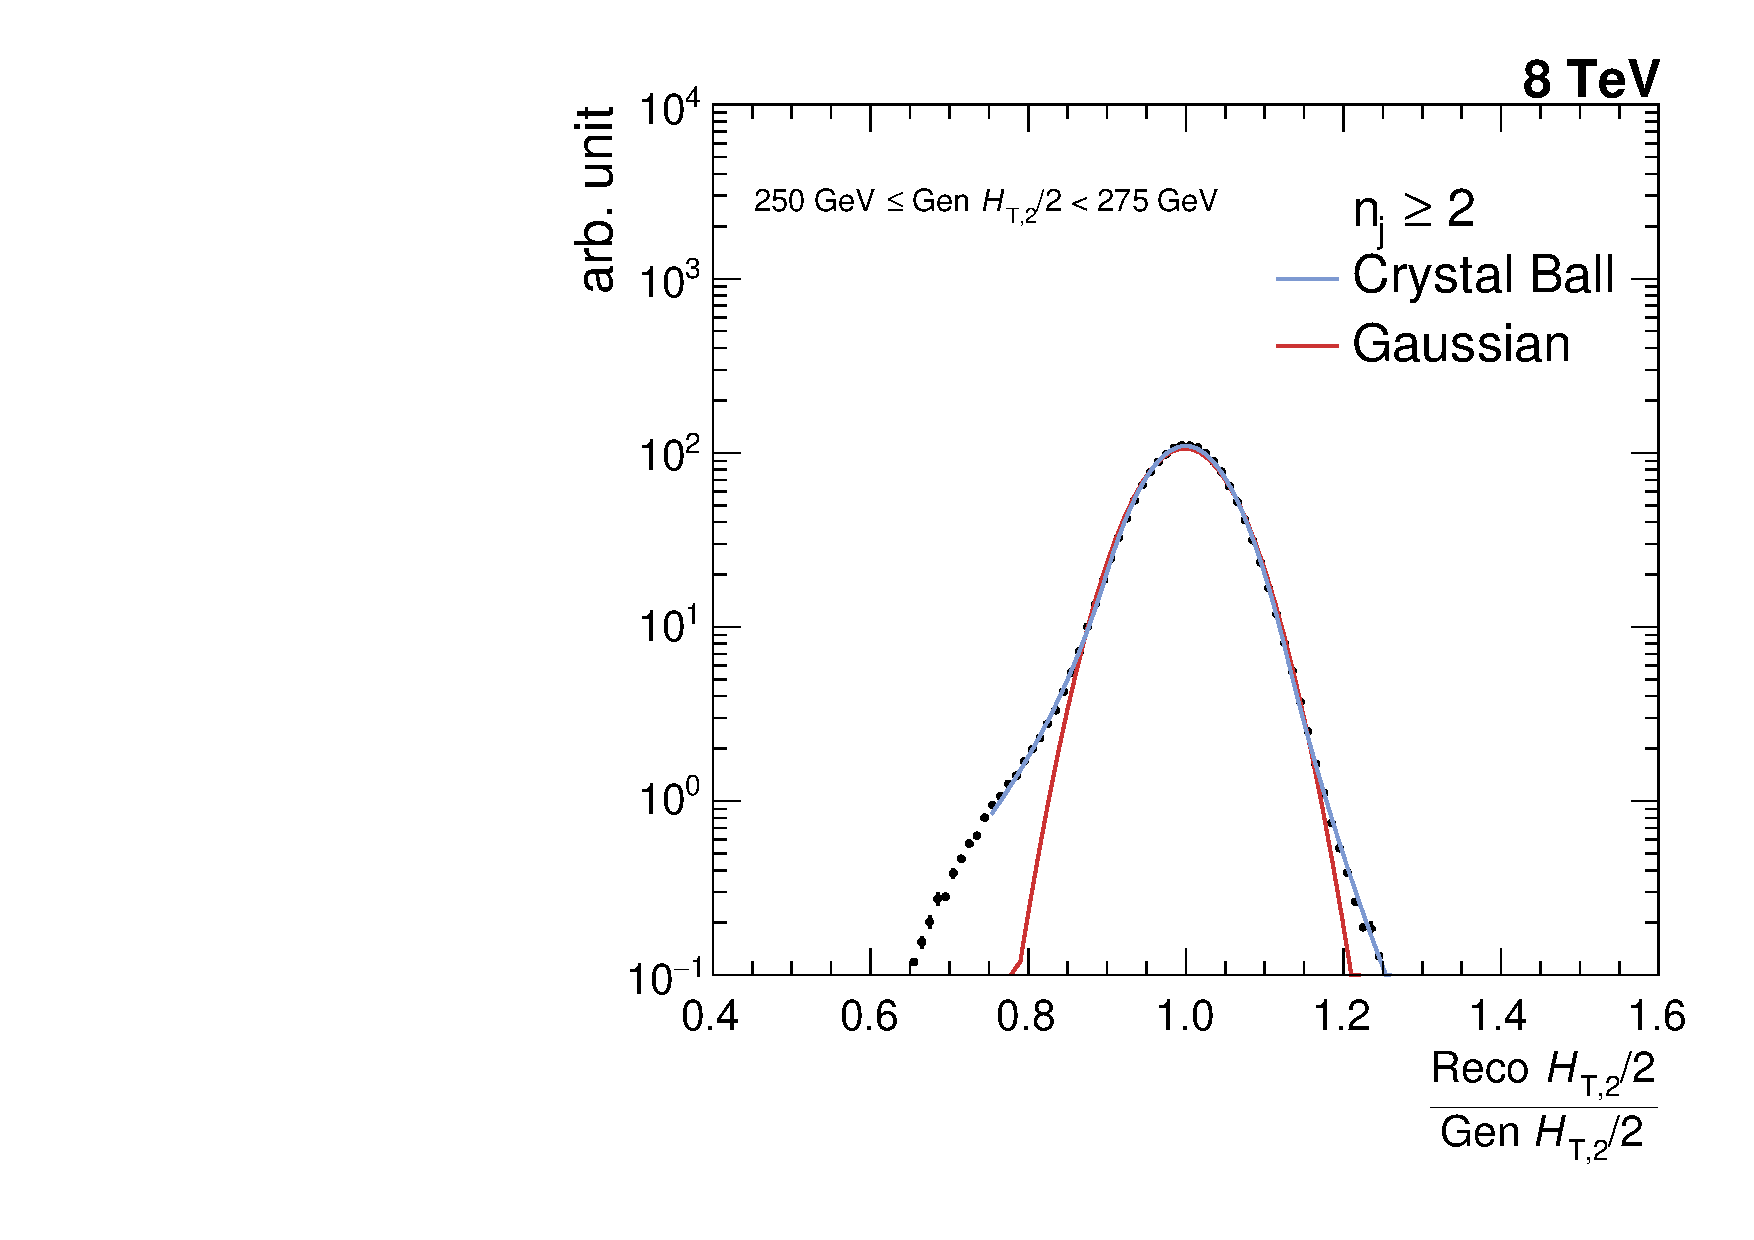
\includegraphics[width=0.51\textwidth]{Plots_HT_2_150/Fit_Res_2_final_crystal_genbin_250-275_crystal_nomet.pdf}%
 ~~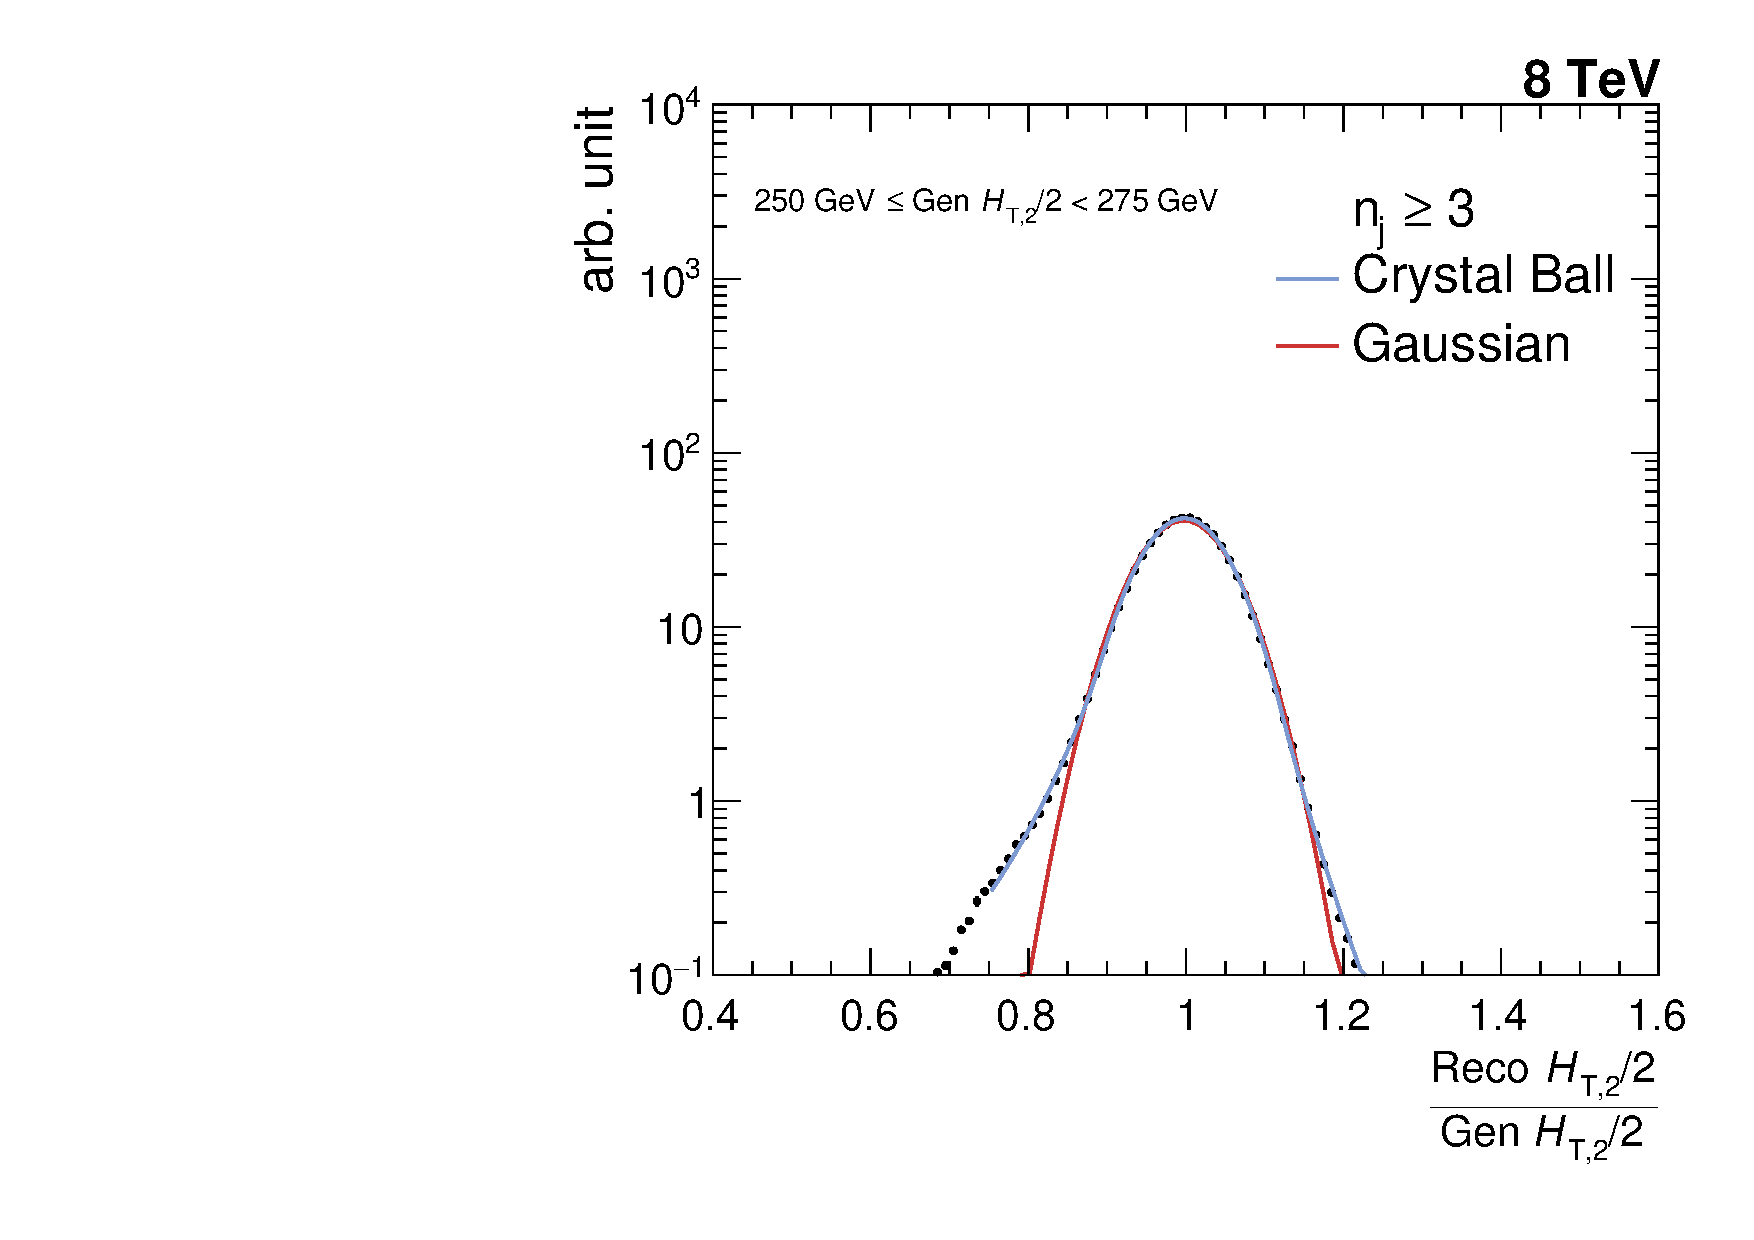
\includegraphics[width=0.51\textwidth]{Plots_HT_2_150/Fit_Res_3_final_crystal_genbin_250-275_crystal_nomet.pdf}
 \caption[Fitting of the jet energy resolution distribution as a function of \httwo.]{Fitting of the jet energy resolution distribution, obtained using LO \MadGraphFn\plusn \PYTHIAS (\MGP) Monte Carlo simulated events, as a function of \httwo for inclusive 2-jet (left) and 3-jet events (right). The blue line shows the double-sided Crystal Ball function fit of $\frac{{\rm Reco}~\httwo}{{\rm Gen}~\httwo}$ in each Gen \httwo bin, overlayed by Gaussian fitting the core of the resolution (red line).}
 \label{fig:fit_gauss}
 \end{center}
\end{figure}

The width of the response distribution in a given Gen \httwo bin is interpreted as the resolution which in good approximation can be described by the $\sigma$ of a Gaussian fit of the response distribution. A double-sided Crystal-Ball function takes into account the non-Gaussian tails of the jet response distribution. The resolution as a function of \httwo is calculated separately for both \njt~and \njth~events. A fit example for one Gen \httwo bin is shown in Fig.~\ref{fig:fit_gauss} for \njt~(left) and 3-jet events (right). Here the black dots represent the jet response distribution and the double-sided Crystal-Ball fit (blue line) is overlayed by the Gaussian fit (red line). The resolution in each Gen \httwo bin is then plotted as a function of Gen \httwo. 

\begin{figure}[!h]
 \begin{center}
 \hspace*{-5mm}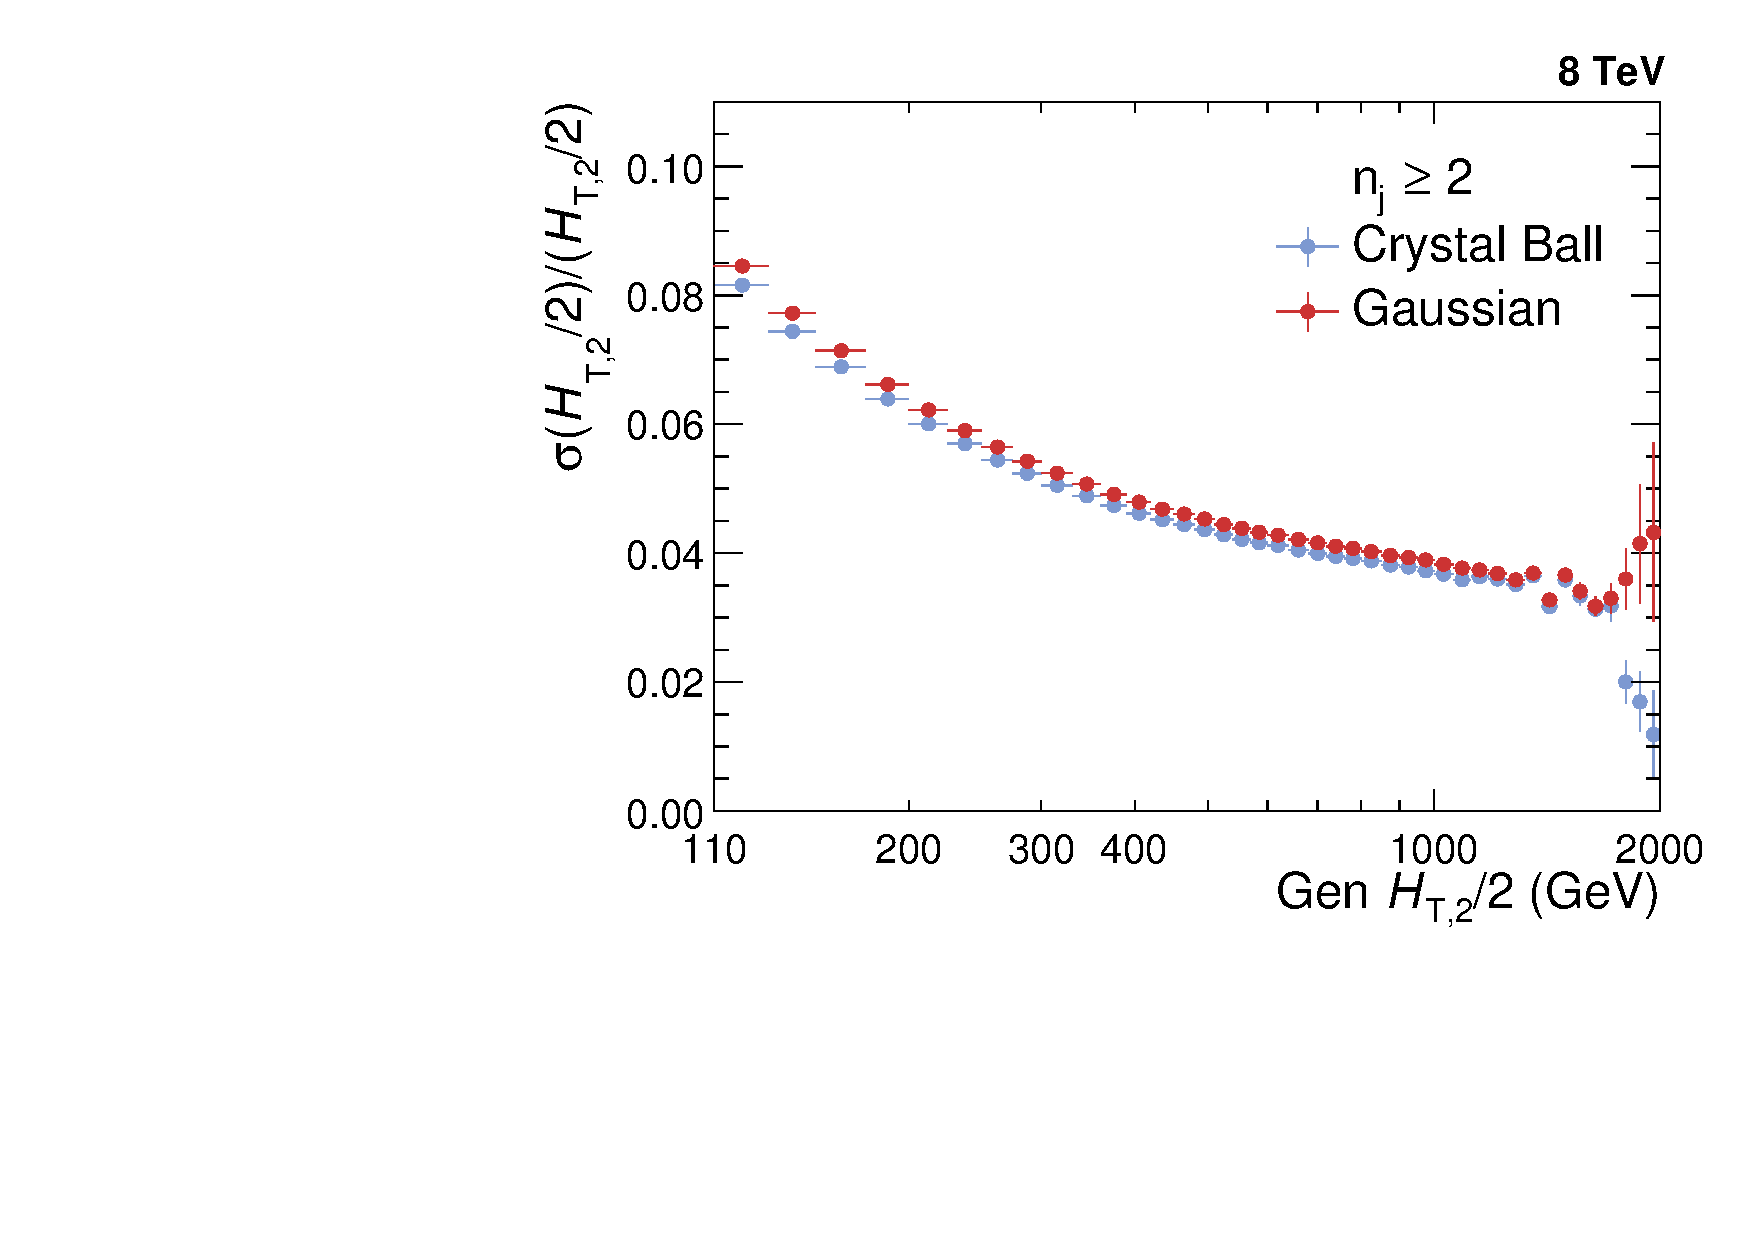
\includegraphics[width=0.51\textwidth]{Plots_HT_2_150/Comparison_Resolution_Crystal_Gauss_2.pdf}%
 ~~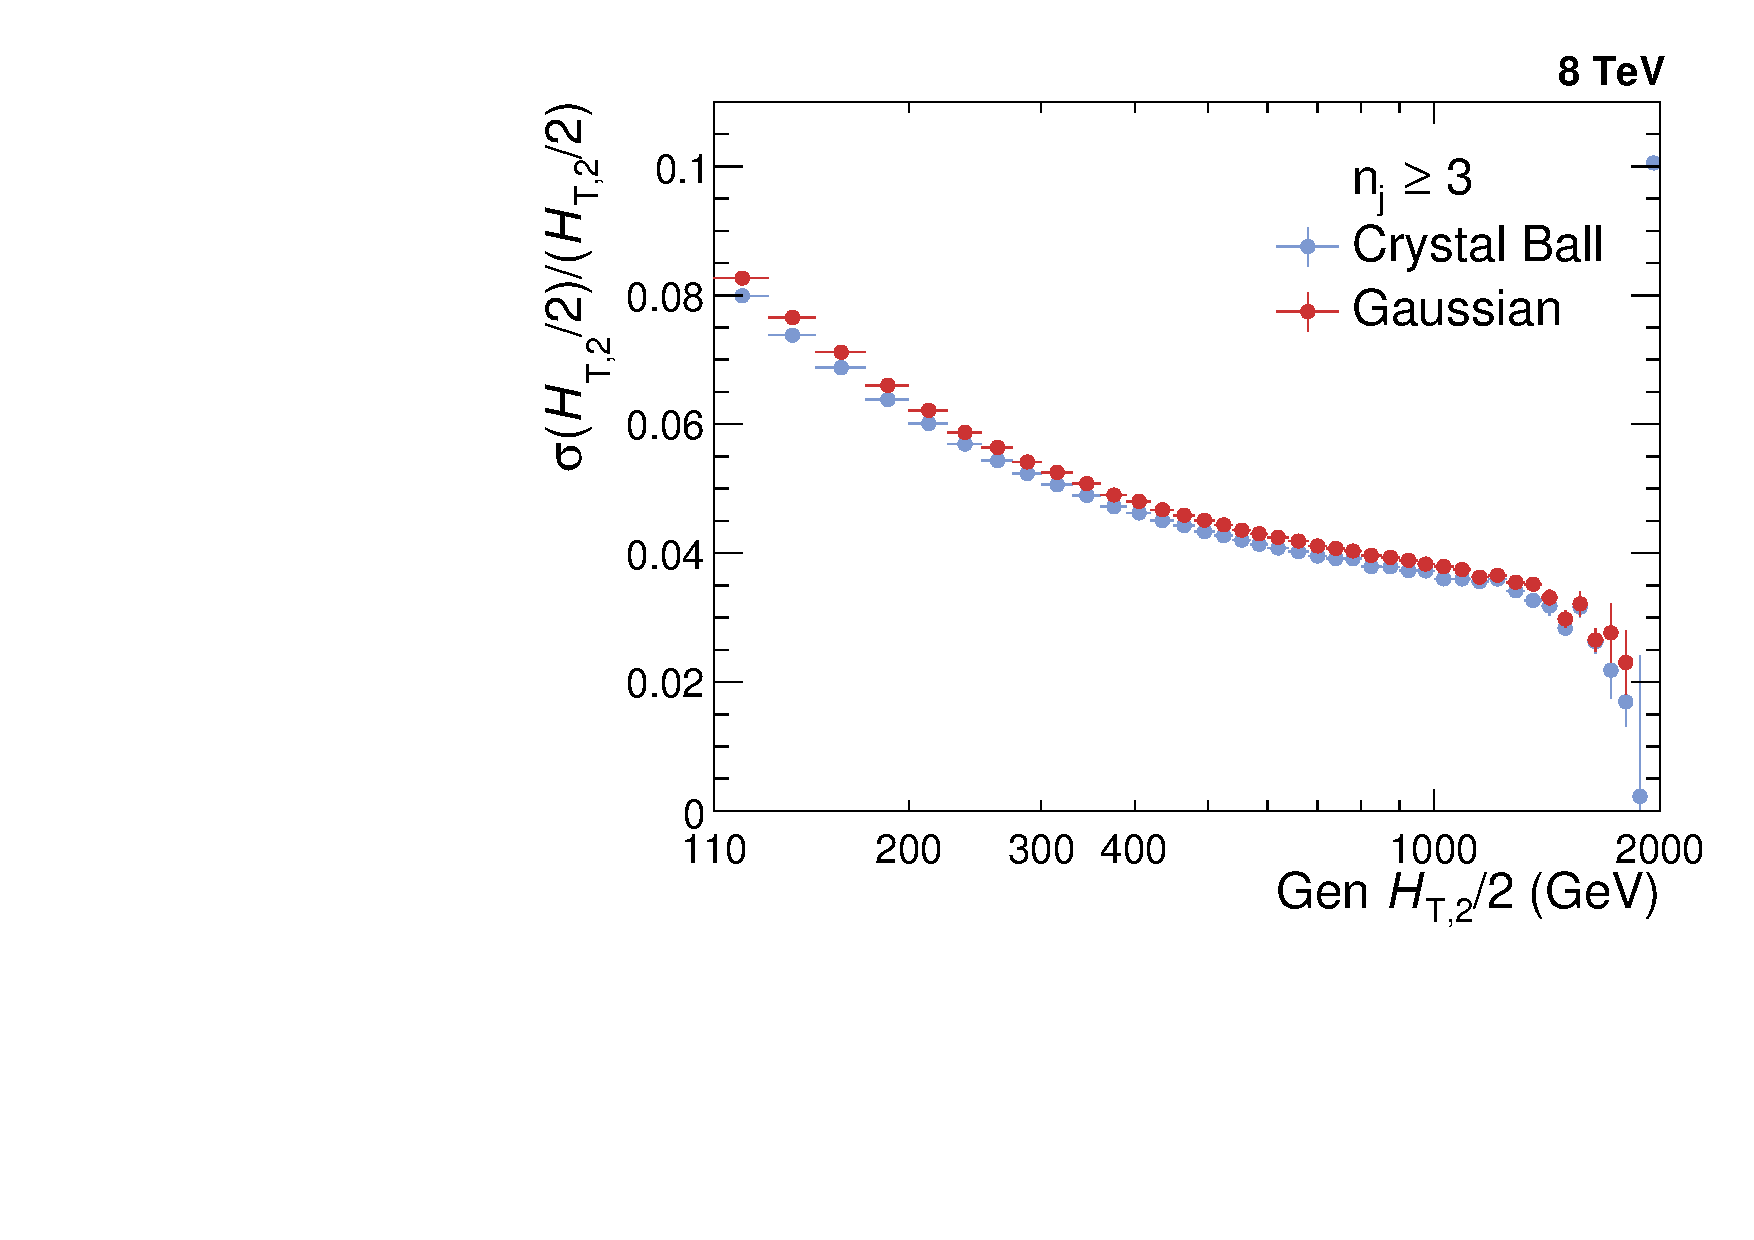
\includegraphics[width=0.51\textwidth]{Plots_HT_2_150/Comparison_Resolution_Crystal_Gauss_3.pdf}
 \caption[Comparison of jet energy resolution calculated using Crystal-Ball fit function and Gaussian fit function]{Comparison of jet energy resolution calculated using Crystal-Ball fit function (blue solid circles) and Gaussian fit function (red solid circles) for inclusive 2-jet (left) and 3-jet events (right).}
 \label{fig:res_comp}
 \end{center}
\end{figure}

\begin{figure}[!h]
 \begin{center}
 \hspace*{-5mm}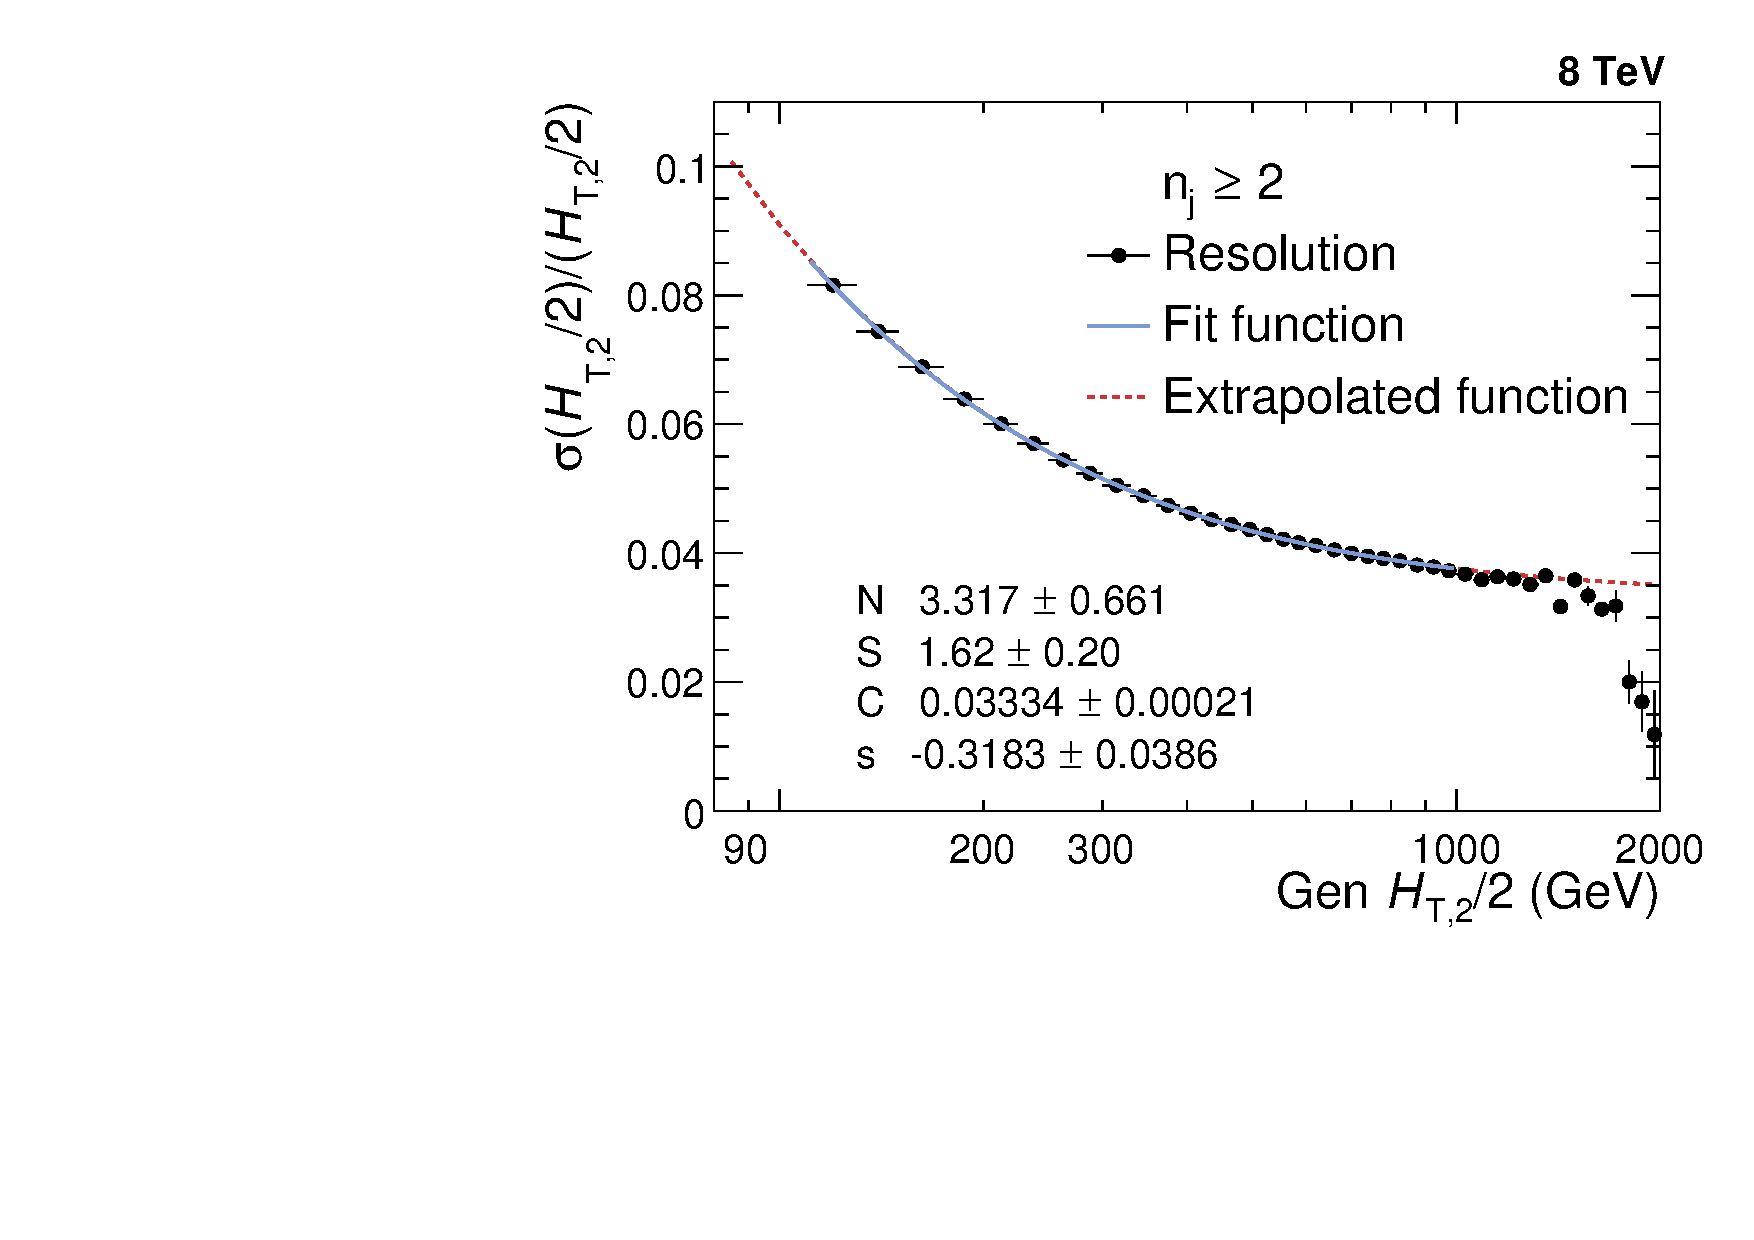
\includegraphics[width=0.51\textwidth]{Plots_HT_2_150/Extrapolate_Sigma_Value_Res_2_crystal_range_ext.pdf}%
 ~~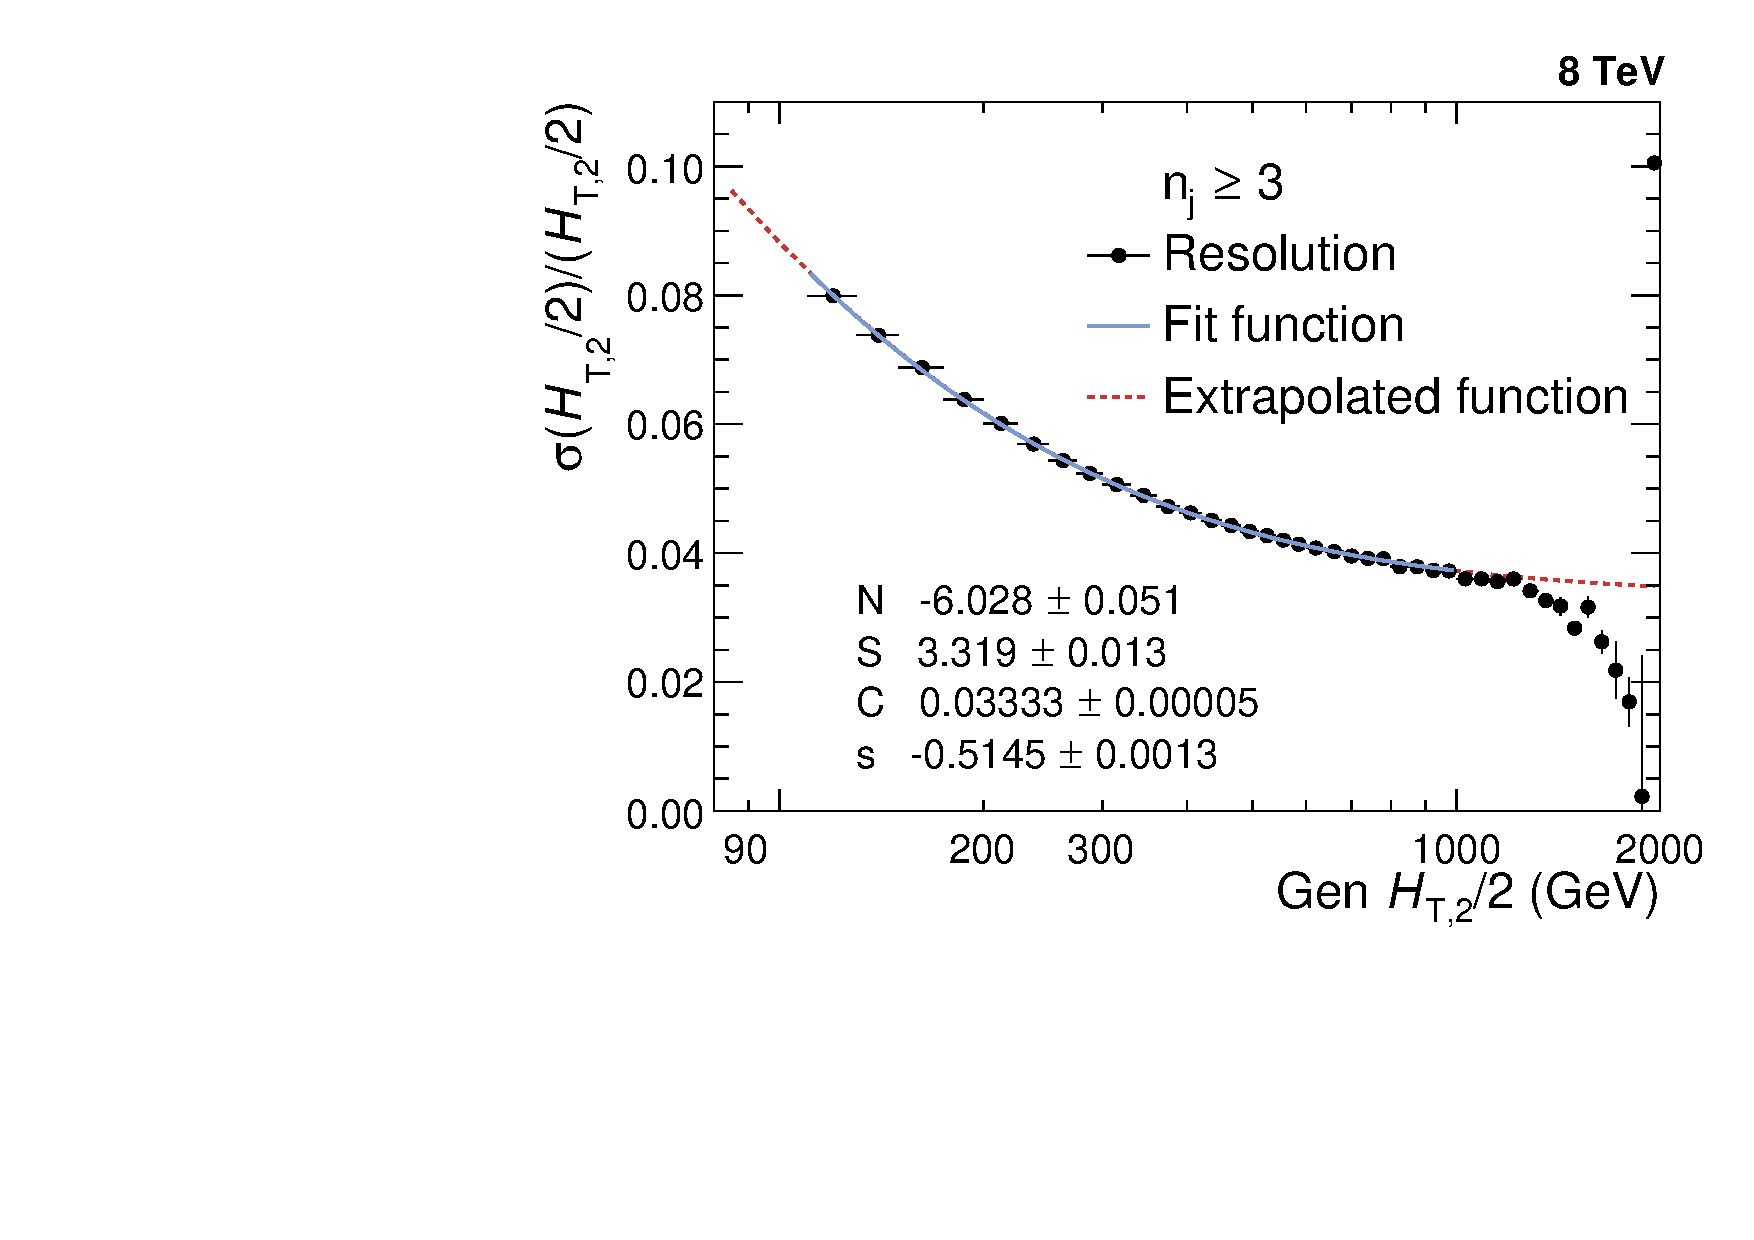
\includegraphics[width=0.51\textwidth]{Plots_HT_2_150/Extrapolate_Sigma_Value_Res_3_crystal_ext.pdf}
 \caption[Jet energy resolution (JER) is shown as a function of Gen \httwo.]{Jet energy resolution (JER) is shown as a function of Gen \httwo for inclusive 2-jet (left) and 3-jet events (right). JER (black solid circles) is fitted by using the modified NSC-formula (blue solid line) which is extrapolated to 80 GeV and up to 2000 GeV (red dashed line) to consider the migration into lower as well as higher bins.}
 \label{fig:resolution}
 \end{center}
\end{figure}
 
As expected, it has been observed from Fig.~\ref{fig:res_comp} that the Crystal Ball function (blue solid circles) describes the measured distributions better as compared to Gaussian function fit (red solid circles), especially in the low-\httwo region where the non-Gaussian tails are more pronounced. Hence JER is determined using Crystal Ball function fit. Figure~\ref{fig:resolution} shows the final relative jet energy resolution (JER) which is described by a modified version of the NSC formula (blue solid line) \cite{CMS:2011esa}, as mentioned in Equation~\ref{NSC_formula}. To consider the migration to lower as well higher bins and to obtain the resolution with reasonable statistics over the full range of Gen \httwons, the fit function is extrapolated to 80 GeV and up to 2000 GeV which is shown by red dashed line. The fit formula used here is basically the usual NSC formula which describes the resolution in terms of noise $N$ originating due to electronic and pileup noise and is independent of \httwons; a stochastic component $S$ due to sampling fluctuation and EM fraction fluctuation per hadrons; and a constant term $C$ because of dead material, magnetic field and calorimeter cell to cell fluctuation. In the low \httwo region the tracking has a non-negligible influence on the resolution due to the particle flow algorithm, so the additional parameter $s$ is introduced to obtain slightly better fits. The parameters obtained after fitting the relative resolution using the above mentioned NSC formula are tabulated in Table~\ref{fit_para} for \njt~and \njth~events. This calculated JER is used in unfolding procedure to smear the generated truth spectrum which is used as input in getting the response matrices and is explained in details in Sec.~\ref{sec:funcs}. Since JER in \njt~events is similar to that one in \njth~events, so N, S and C fit parameters obtained for \njth~events are used for unfolding \rations.

\begin{equation}
 \label{NSC_formula}
 \frac{\sigma (x)}{x} = \sqrt{sgn(N) \cdot\frac{N^{2}}{x^{2}}+S^{2}\cdot x^{s-1}+C^{2}} 
\end{equation}

\begin{table}[!h]
 \centering
 \caption[The parameters obtained by fitting the relative resolution as a function of \httwons.]{The parameters obtained by fitting the relative resolution as a function of \httwons, using the modified NSC formula, for inclusive 2-jet and 3-jet events.}
 \label{fit_para}
 \vspace{2mm}
 \begin{tabular}{ccccc}
 \hline \hline
 &    N    &  S   &    C   &    s   \rbtrr \\ \hline
 Inclusive 2-jet  & ~3.32 & 1.62 & 0.0333 & -0.318  \rbtrr \\
 Inclusive 3-jet  & -6.03 & 3.32 & 0.0333 & -0.515  \rbtrr \\
 \hline \hline
 \end{tabular}
\end{table}

%Since the JER is calculated using \MGP~Reco and Gen \httwo distributions, so it is expected that the Gen \httwo smeared using this JER should match the Reco \httwo. But this extracted JER in one large rapidity bin, smears the Gen \httwo too much because \textcolor{myred}{$\rm {\frac{Smeared~Gen}{Gen}}$} does not matches with simulated \textcolor{blue}{$\rm {\frac{Reco}{Gen}}$} as observed in Fig.~\ref{fig:ratios} for \njt~(left) and \njth~events (right). When the 30\% reduced JER is used to smear Gen, then \textcolor{pink}{$\rm {\frac{Smeared~Gen}{Gen}}$} matches with simulated \textcolor{blue}{$\rm {\frac{Reco}{Gen}}$} ignoring the statistical fluctuations. So an additional unfolding uncertainty is attributed by comparison to 30\% reduced JER.

Since the JER is calculated using \MGP~Reco and Gen \httwo distributions, so it is expected that if Gen \httwo is smeared using this JER, it should match the Reco \httwo. But this extracted JER in one large rapidity bin, smears the Gen \httwo too much because Smeared Gen/Gen ratio (red line) shows a discrepancy from simulated Reco/Gen ratio (blue line), as observed in Fig.~\ref{fig:ratios} for \njt~(left) and \njth~events (right). Some shortcomings in the detector simulation of the theory spectra leads to these small nonclosures. When the 30\% reduced JER is used to smear Gen, then the ratio Smeared Gen/Gen (pink line) matches with simulated Reco/Gen ratio (blue line) within the statistical fluctuations. Hence an additional unfolding uncertainty is attributed by comparison to 30\% reduced JER for both \njt~and \njth~events. Due to high statistical fluctuations at high \httwons, range is presented up to 1680 GeV only.

\begin{figure}[!htbp]
 \begin{center}
 \hspace*{-5mm}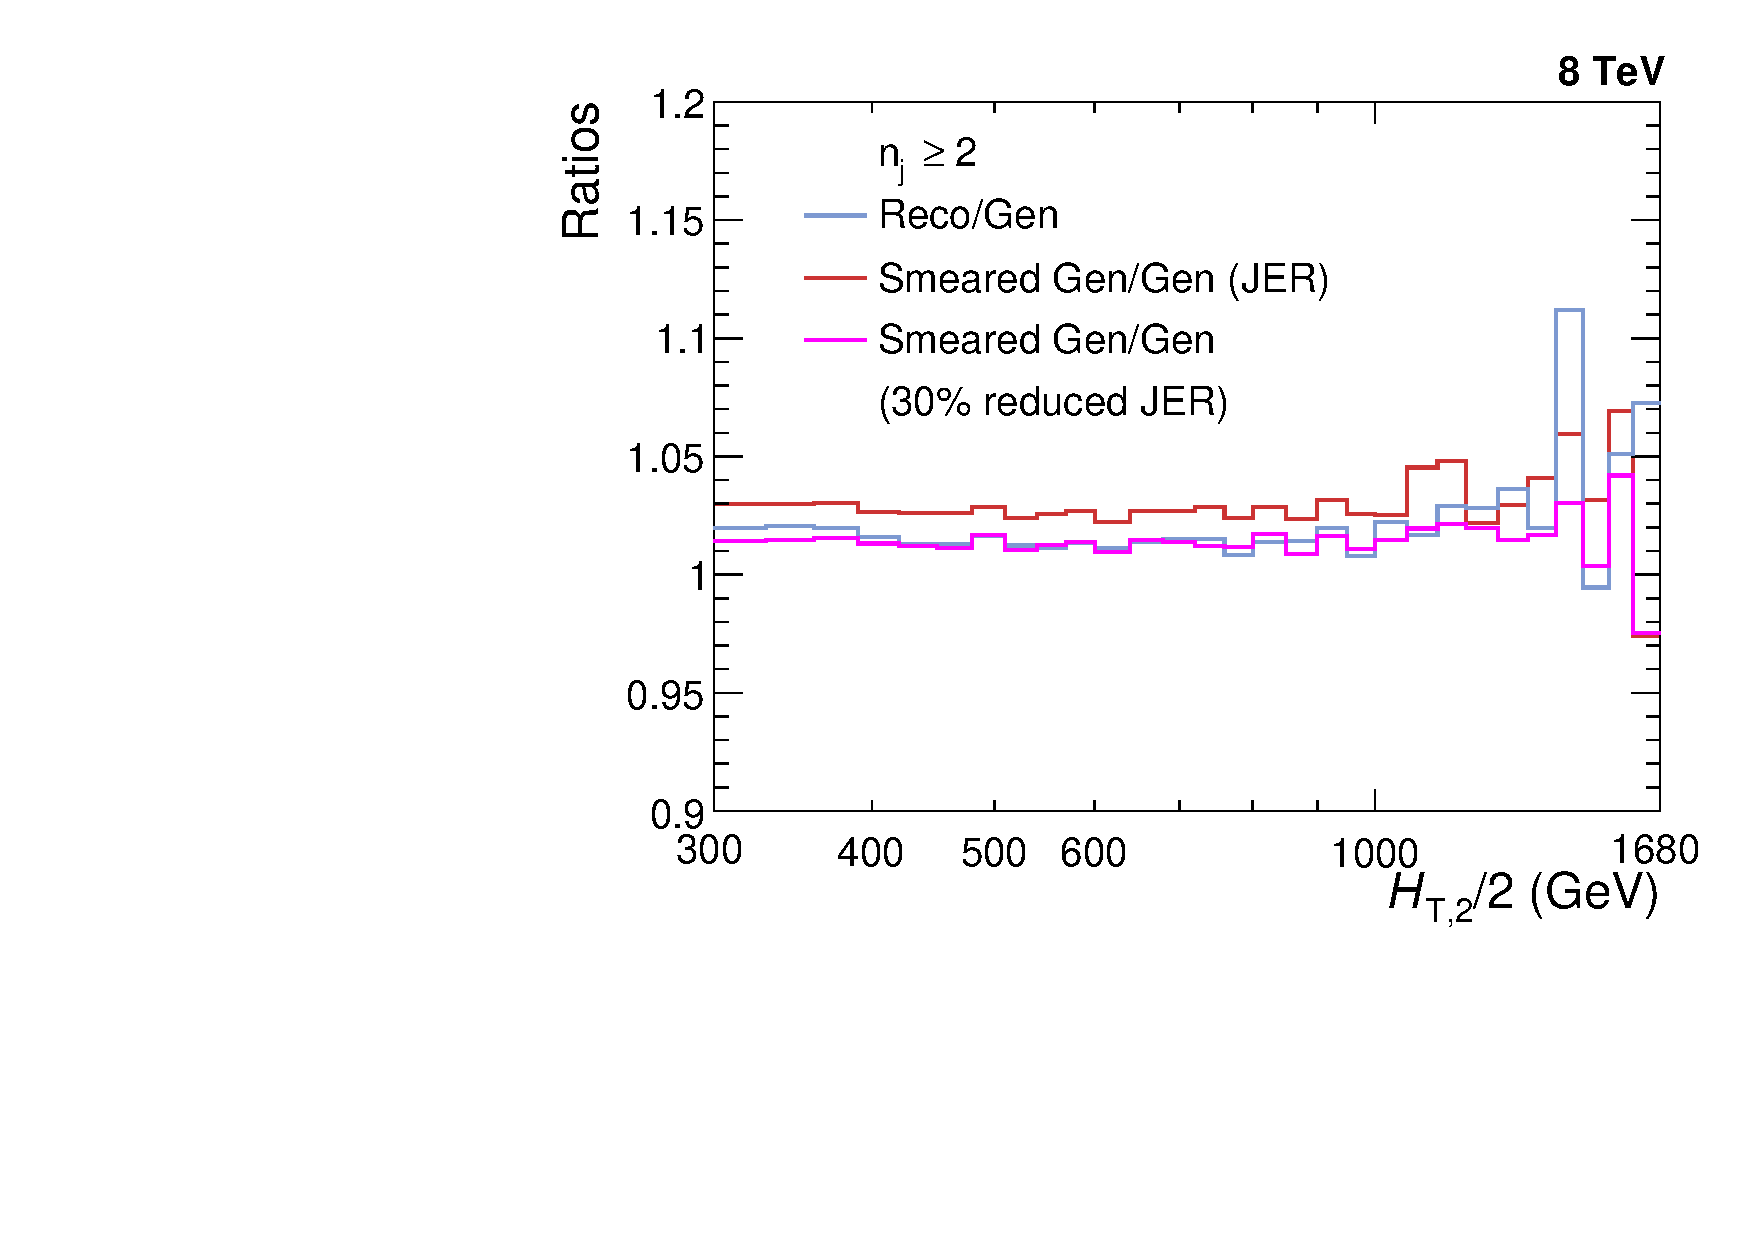
\includegraphics[width=0.51\textwidth]{Plots_HT_2_150/Ratio_Reco_2_crystal.pdf}%
 ~~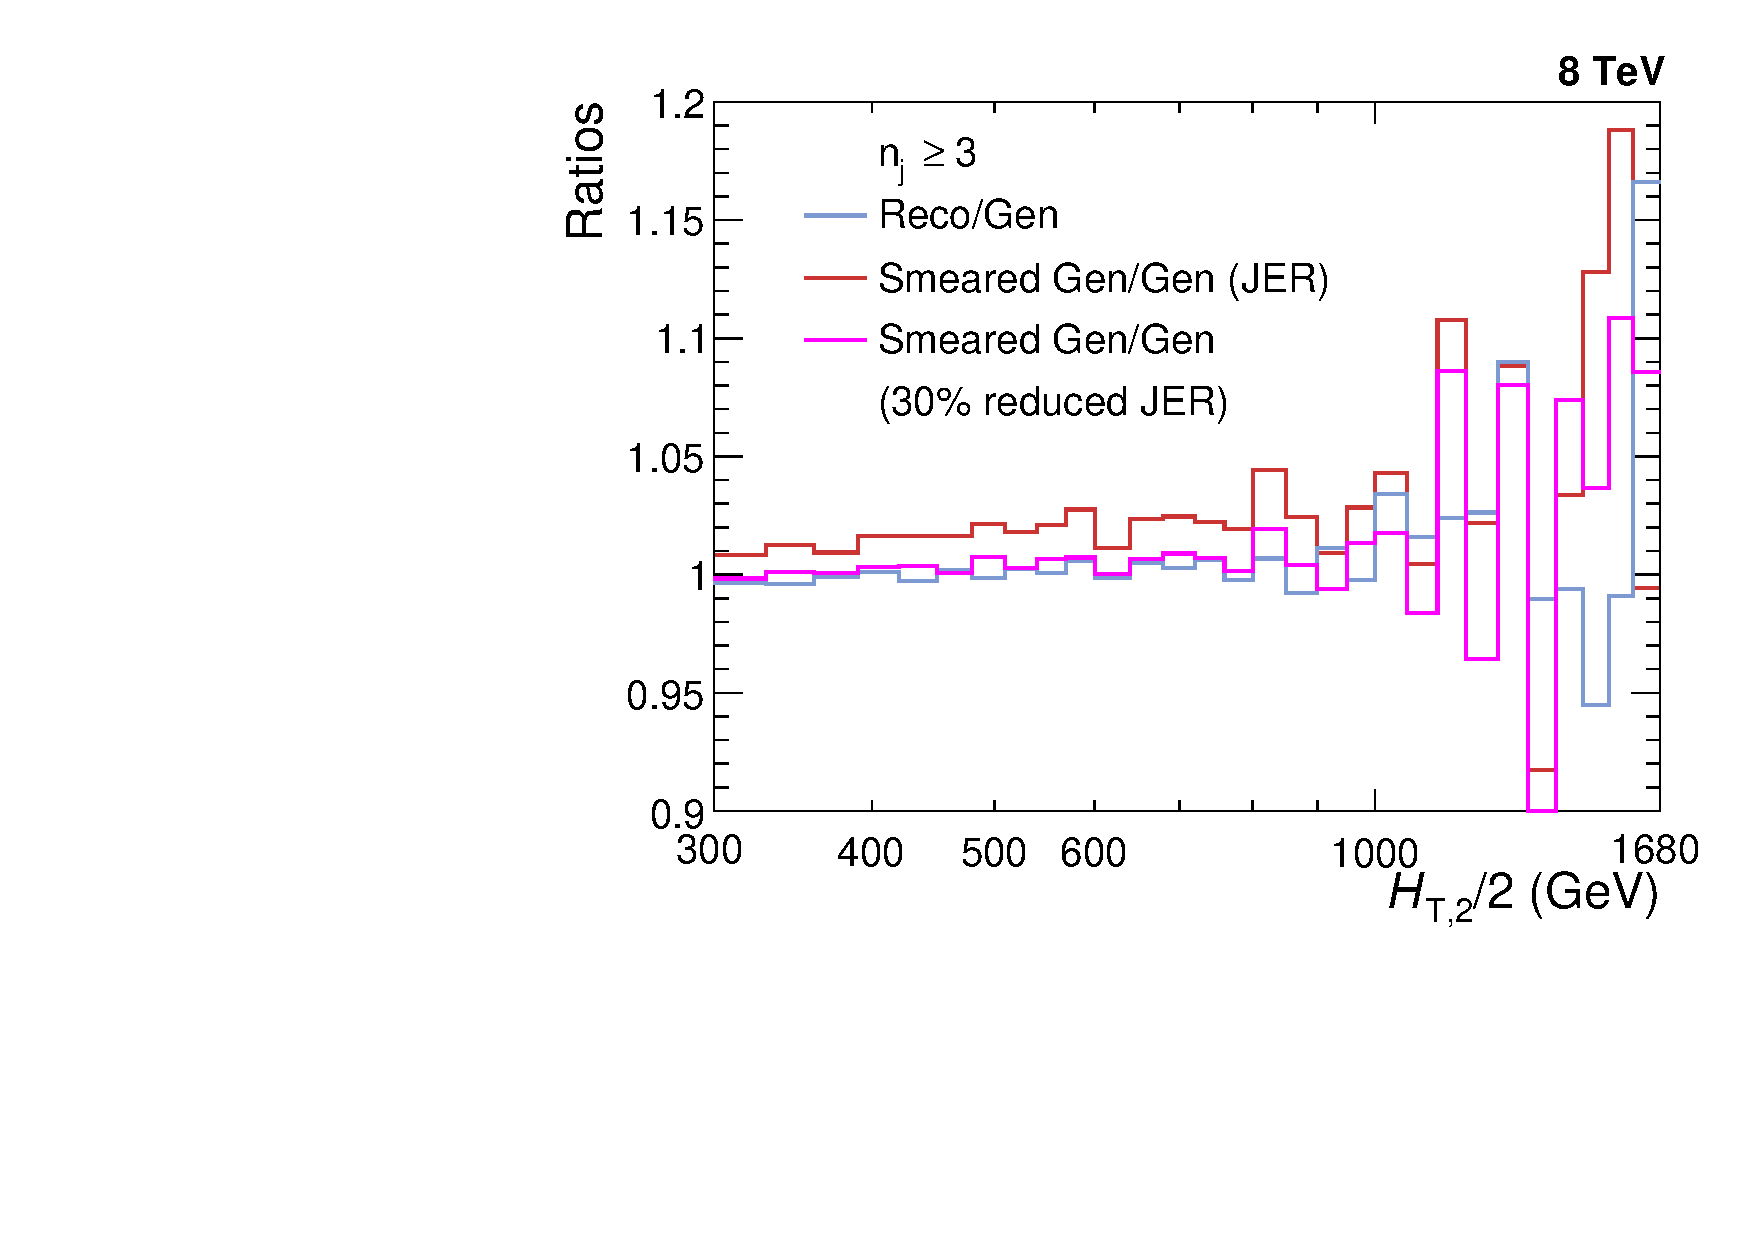
\includegraphics[width=0.51\textwidth]{Plots_HT_2_150/Ratio_Reco_3_crystal.pdf}
 \caption[Additional unfolding uncertainty.]{\MadGraphFn\plusn \PYTHIAS (\MGP) Gen smeared using extracted jet energy resolution (JER) shows a discrepancy from simulated Reco as Smeared Gen/Gen ratio (red line) does not match with Reco/Gen ratio (blue line), for both inclusive 2-jet (left) and 3-jet events (right). Smeared Gen/Gen ratio (pink line) where Gen is smeared using 30\% reduced JER matches with simulated Reco/Gen ratio (blue line) within the statistical fluctuations. Hence an additional unfolding uncertainty is attributed by comparison to 30\% reduced JER.}
 \label{fig:ratios}
 \end{center}
\end{figure}

\section{Unfolding}
\label{sec:unfolding}
One of the main goals in an experimental measurement is to do the comparison of data with theory predictions or with the results obtained from other experiments. But the finite resolution of a detector and the steeply falling jet \pt spectrum distorts the physical quantities. As a result, the measured observables are different from their corresponding true values. Each \pt bin content contains the migrated events from neighbouring bins along with the original events. So an unfolding process of the data should be followed in order to remove detector effects. In this analysis, the measurements are corrected for detector smearing effects and unfolded to stable particle level by using the iterative D$'$Agostini Bayesian algorithm \cite{DAgostini:1994fjx,DAgostini} as implemented in RooUnfold software package \cite{Adye:2011gm}. In this algorithm, the number of iterations regularize the unfolding process. The obtained distribution in one iteration is taken as the input in the next one. \chisq between two successive iterations is given by Eq.~\ref{eq:bayes_chi}. The number of iterations stop when \chisq/$N_{bins}$ is \ls 1. A reduced \chisq is obtained by a higher number of iterations but this will also increase the uncertainty and there are larger bin-by-bin fluctuations and correlations. So the optimization of number of iterations is very important. In the current analysis, unfolding done with ``four'' iterations gives the best results with low \chisq and low bin-by-bin correlations.

\begin{equation}
\label{eq:bayes_chi}
\chisq = \sum\limits_{i=1}^{N_{bins}}\bigg(\frac{n^{j\plusn}_{i} - n^{j}_{i}}{\sqrt{n^{j}_{i}}}\bigg)^{2}
\end{equation} 
where $n^{j}_{i}$ number of events in $i$-th bin for $j$-th iteration. 

The measured differential cross-sections as a function of \httwo, are unfolded separately for \njt~and \njth~events. The measured cross-section ratio \ratio is also corrected for detector smearing effects and unfolded to particle level. There can be two ways to obtain unfolded cross-section ratio :

\begin{itemize}
\item {\bf Method I :} First unfold separately the inclusive 2-jet and 3-jet measured cross-sections and then construct the ratio \ratio 
\item {\bf Method II :} Unfold directly the cross-section ratio \ratio
\end{itemize}

In further analysis, unfolded cross-section ratio \ratio and its systematic uncertainties are calculated using Method I, whereas Method II is used only to propagate the statistical uncertainties including bin-by-bin correlations and statistical correlations between the inclusive 3-jet and 2-jet events cross-sections. Unfolding takes the response matrix as an input which are explained in the next section.

\subsection{Response Matrices}
\label{sec:funcs}
The response matrix is a two dimensional mapping between the true and measured distributions. It is usually derived from simulated Monte Carlo (MC) samples, which takes the true distribution from MC as an input and smears it by taking into account the detector resolution. Then this response matrix is used to unfold the measured data spectrum. But there are several drawbacks of constructing response matrix using this method. In some phase space regions, the shape of the distribution is not well described by the LO predictions. Also, the limited number of events in the MC samples at high transverse momenta introduces high statistical fluctuations in the response matrix. 

However, there is an indirect way of constructing the response matrix which uses a custom Toy Monte Carlo method. In this method, the particle level or true \httwo spectrum is obtained by fitting the theoretically predicted NLO spectrum. Then this distribution is smeared with forward smearing technique, using the extracted jet energy resolution (JER) to obtain the reconstructed level or measured \httwo spectrum. After that, the response matrix is constructed from these two distributions is used for the unfolding procedure. 

\subsubsection{Inclusive Cross-sections}
\label{sec:cross_sec_res}
The NLO spectrum of the differential cross-sections for \njt~and \njth~events obtained using CT10-NLO PDF set are fitted with the following two different functions defined in Eq.~\ref{eq:func1} and~\ref{eq:func2}. These functions describes the shape as well as normalization of the distribution.

\begin{itemize}
\item {\bf Function I : }
  %\end{itemize} 

  \begin{equation}
    \label{eq:func1}
    f(\httwo) = N[x_{T}]^{-a}[1-x_{T}]^{b} \times exp[-c/x_{T}]
  \end{equation}
  where $N$ is normalization factor and $a, b, c$ are fit parameters.\\

  This function is derived from the below function \cite{CMS:2011ab} :
  \begin{equation}
    \label{eq:funcderive}
    f(p_{T};\alpha,\beta,\gamma) = N_{0}[p_{T}]^{-\alpha}\bigg[1-\frac{2~p_{T}~cosh(y_{min})}{\sqrt{s}}\bigg]^{\beta} \times exp[-\gamma/p_{T}]
  \end{equation}
  using 
  \begin{equation}
    \alpha = a,~~\beta = b,~~\gamma = c*\sqrt{s}/2, \\
    x_{T} = \frac{2*\httwons *cosh(y_{min})}{\sqrt{s}} = \frac{2*\httwons}{\sqrt{s}}
  \end{equation}
  where transverse scaling variable $x_{T}$ corresponds to the proton fractional momentum $x$ for dijets with rapidity $y$ = 0, $\sqrt{s}$ = 8000 GeV and $y_{min}$ is low-edge of the rapidity bin $y$ under consideration (here $y_{min}$ is taken equal to 0)
  
\item {\bf Function II : }

  \begin{equation}
    \label{eq:func2}
    f(H_{T,2}/2) = A_{0}\Big(1-\frac{H_{T,2}/2}{A_{6}}\Big)^{A_{7}} \times 10^{F(\httwo)}, {\rm where} ~~~{F(x) = \sum\limits_{i=1}^5 A_{i}\Big(log\big(\frac{x}{A_{6}}\big)\Big)^{i}}
  \end{equation}

  where the parameter $A_{6}$ is fixed to $\frac{\sqrt{s}}{2~cosh(y_{min})}$, where $\sqrt{s}$ = 8000 GeV and $y_{min}$ is 
  the minimum rapidity. The other parameters are derived from the fitting.
\end{itemize}

\begin{figure}[ht]
  \begin{center}
    \hspace*{-5mm}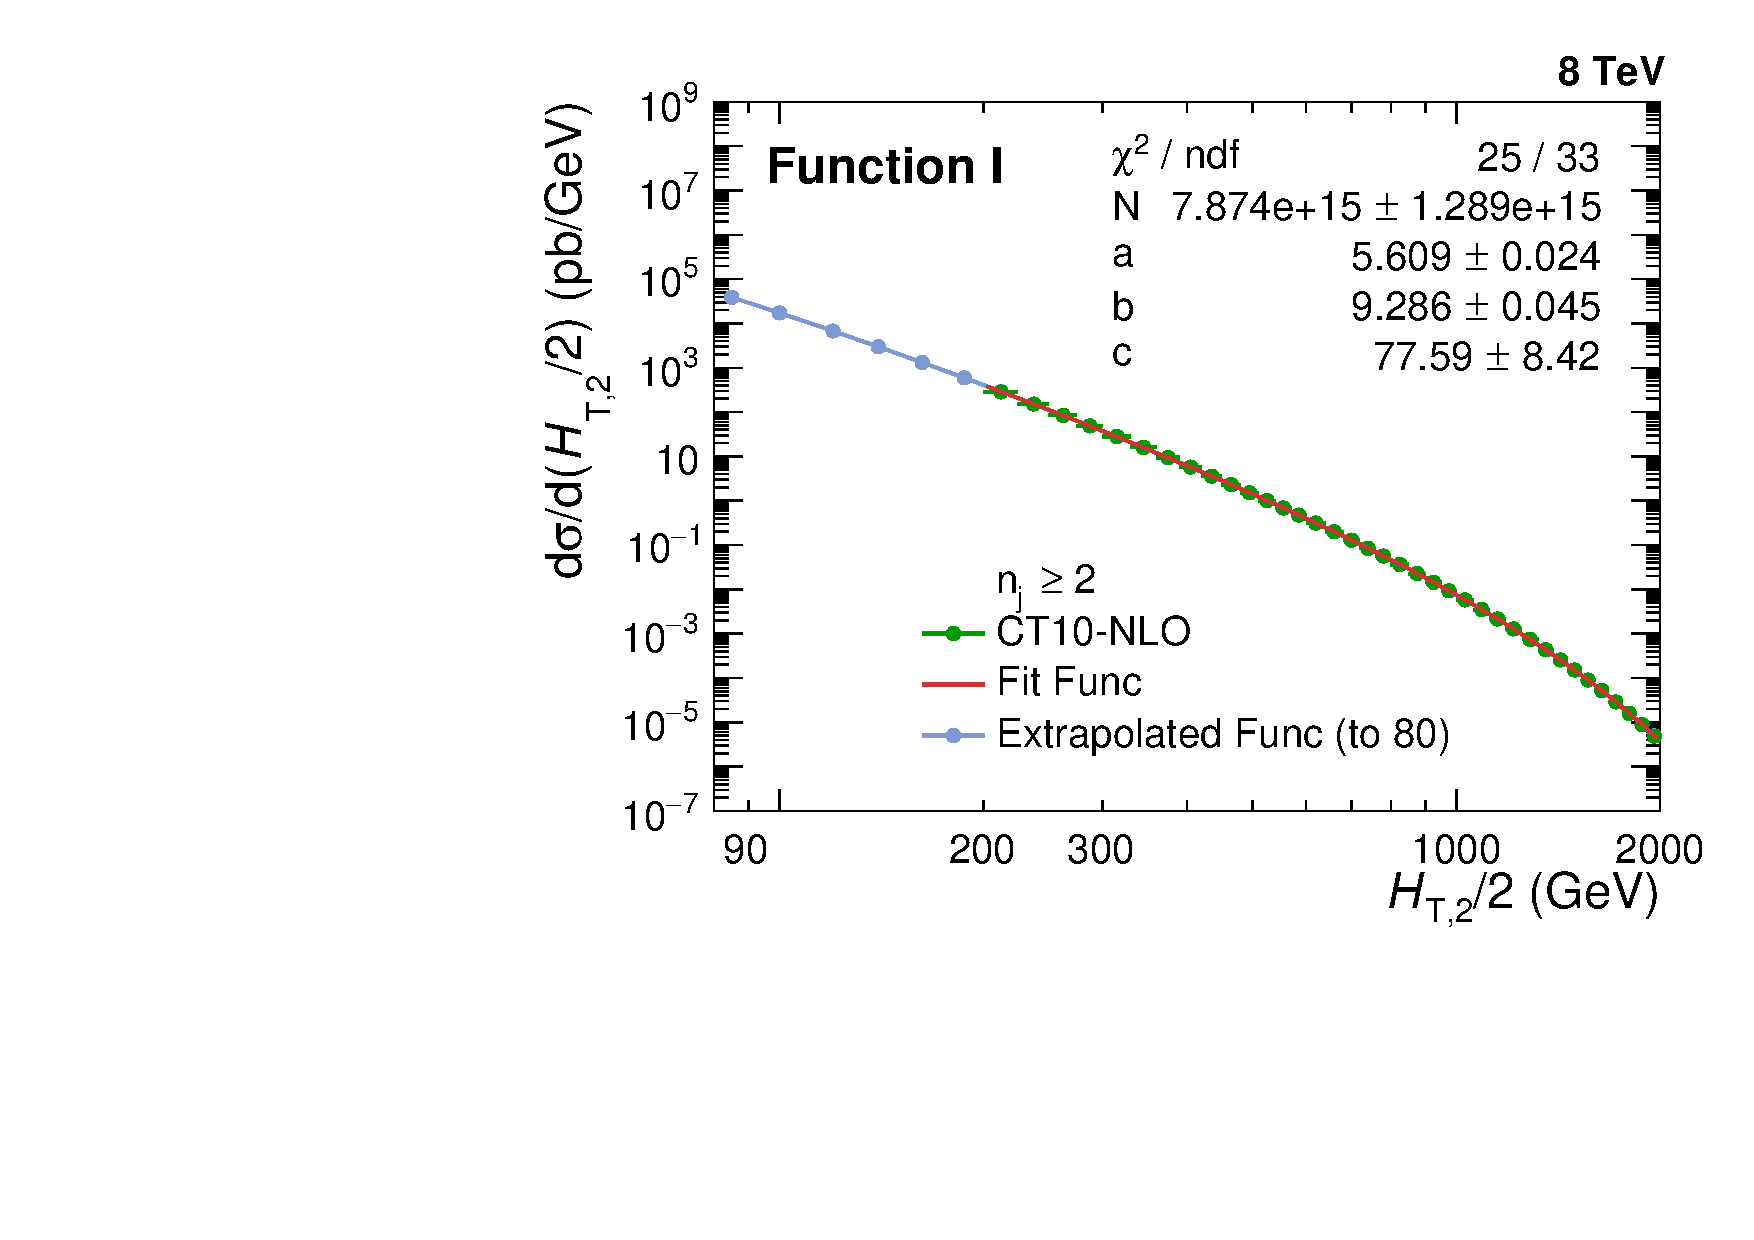
\includegraphics[width=0.51\textwidth]{Plots_HT_2_150/Extrapolate_Theory_2_HT_2_150_funcI.pdf}%
    ~~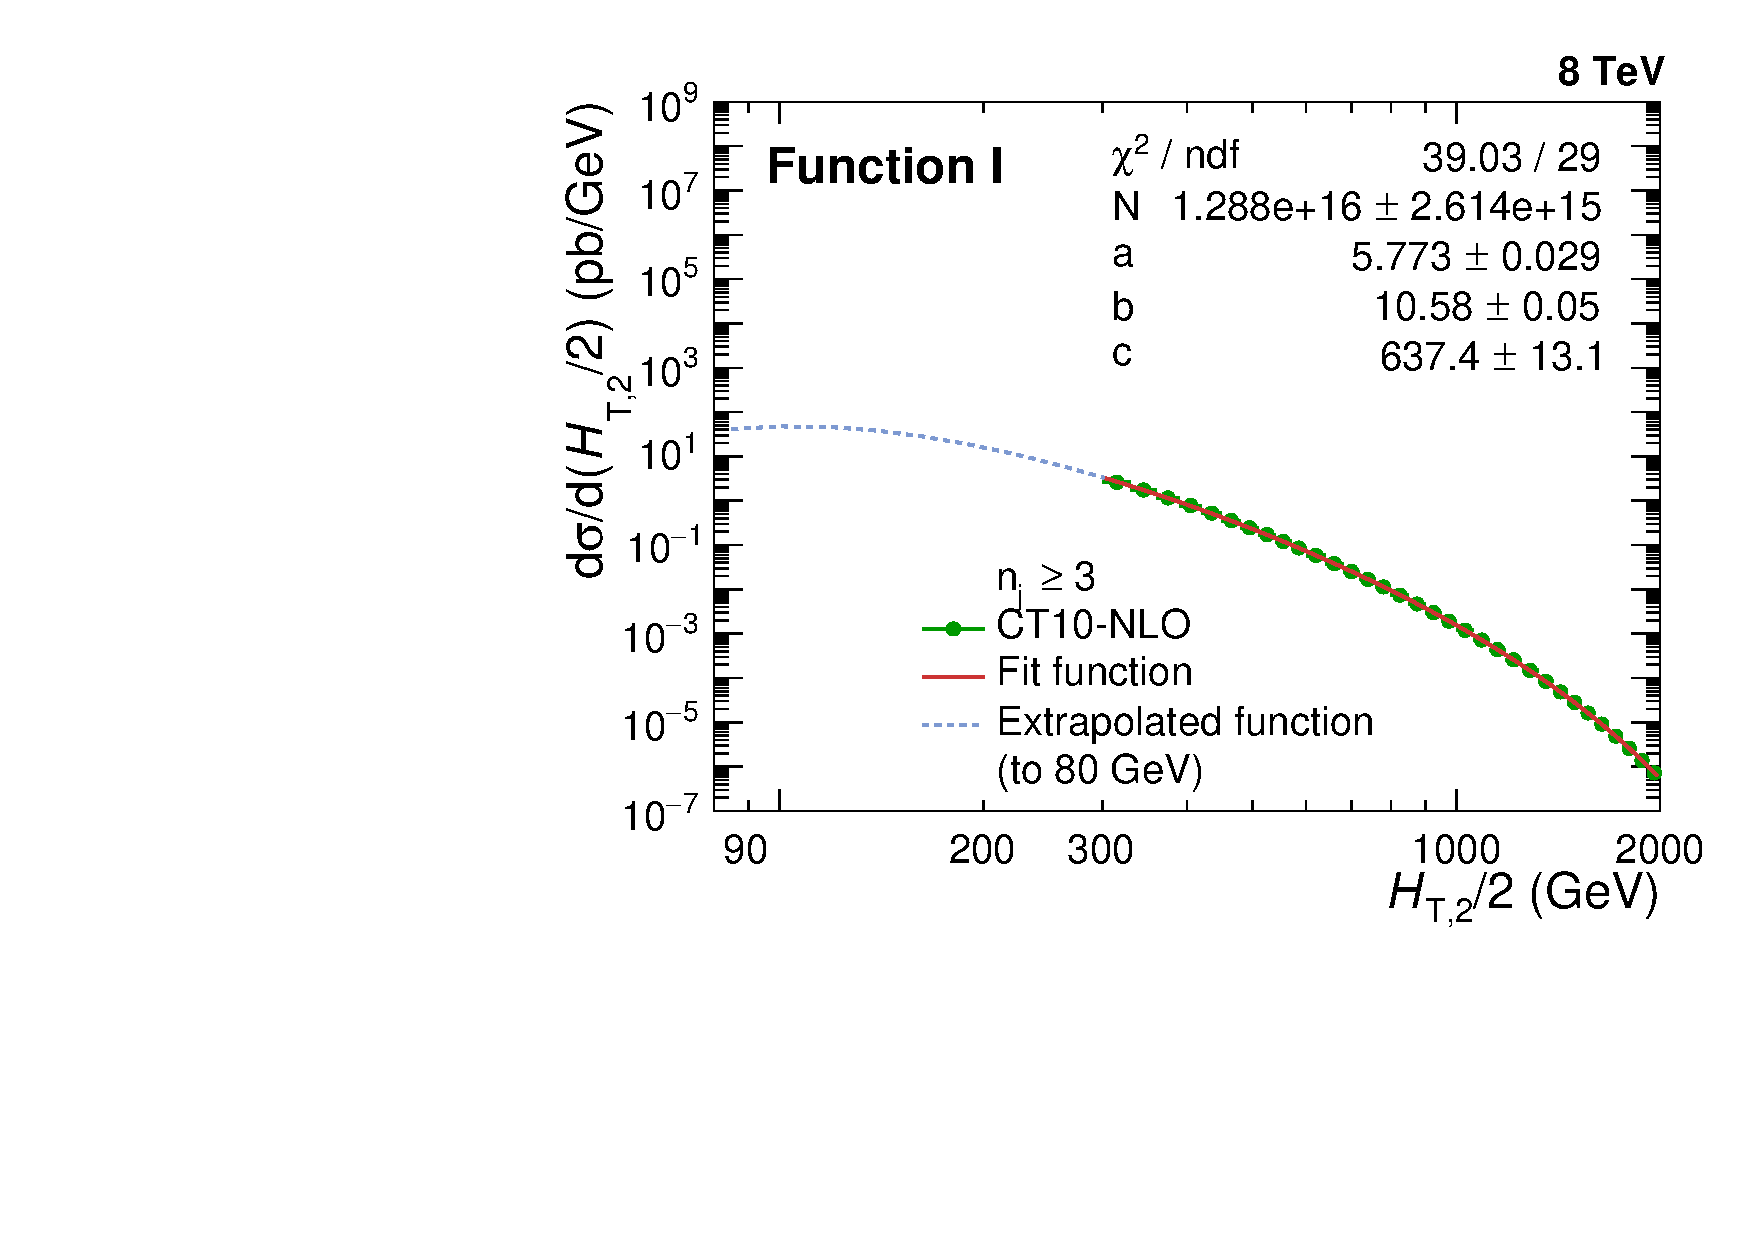
\includegraphics[width=0.51\textwidth]{Plots_HT_2_150/Extrapolate_Theory_3_HT_2_150_funcI.pdf}\\
    \vspace{5mm}
    \hspace*{-5mm}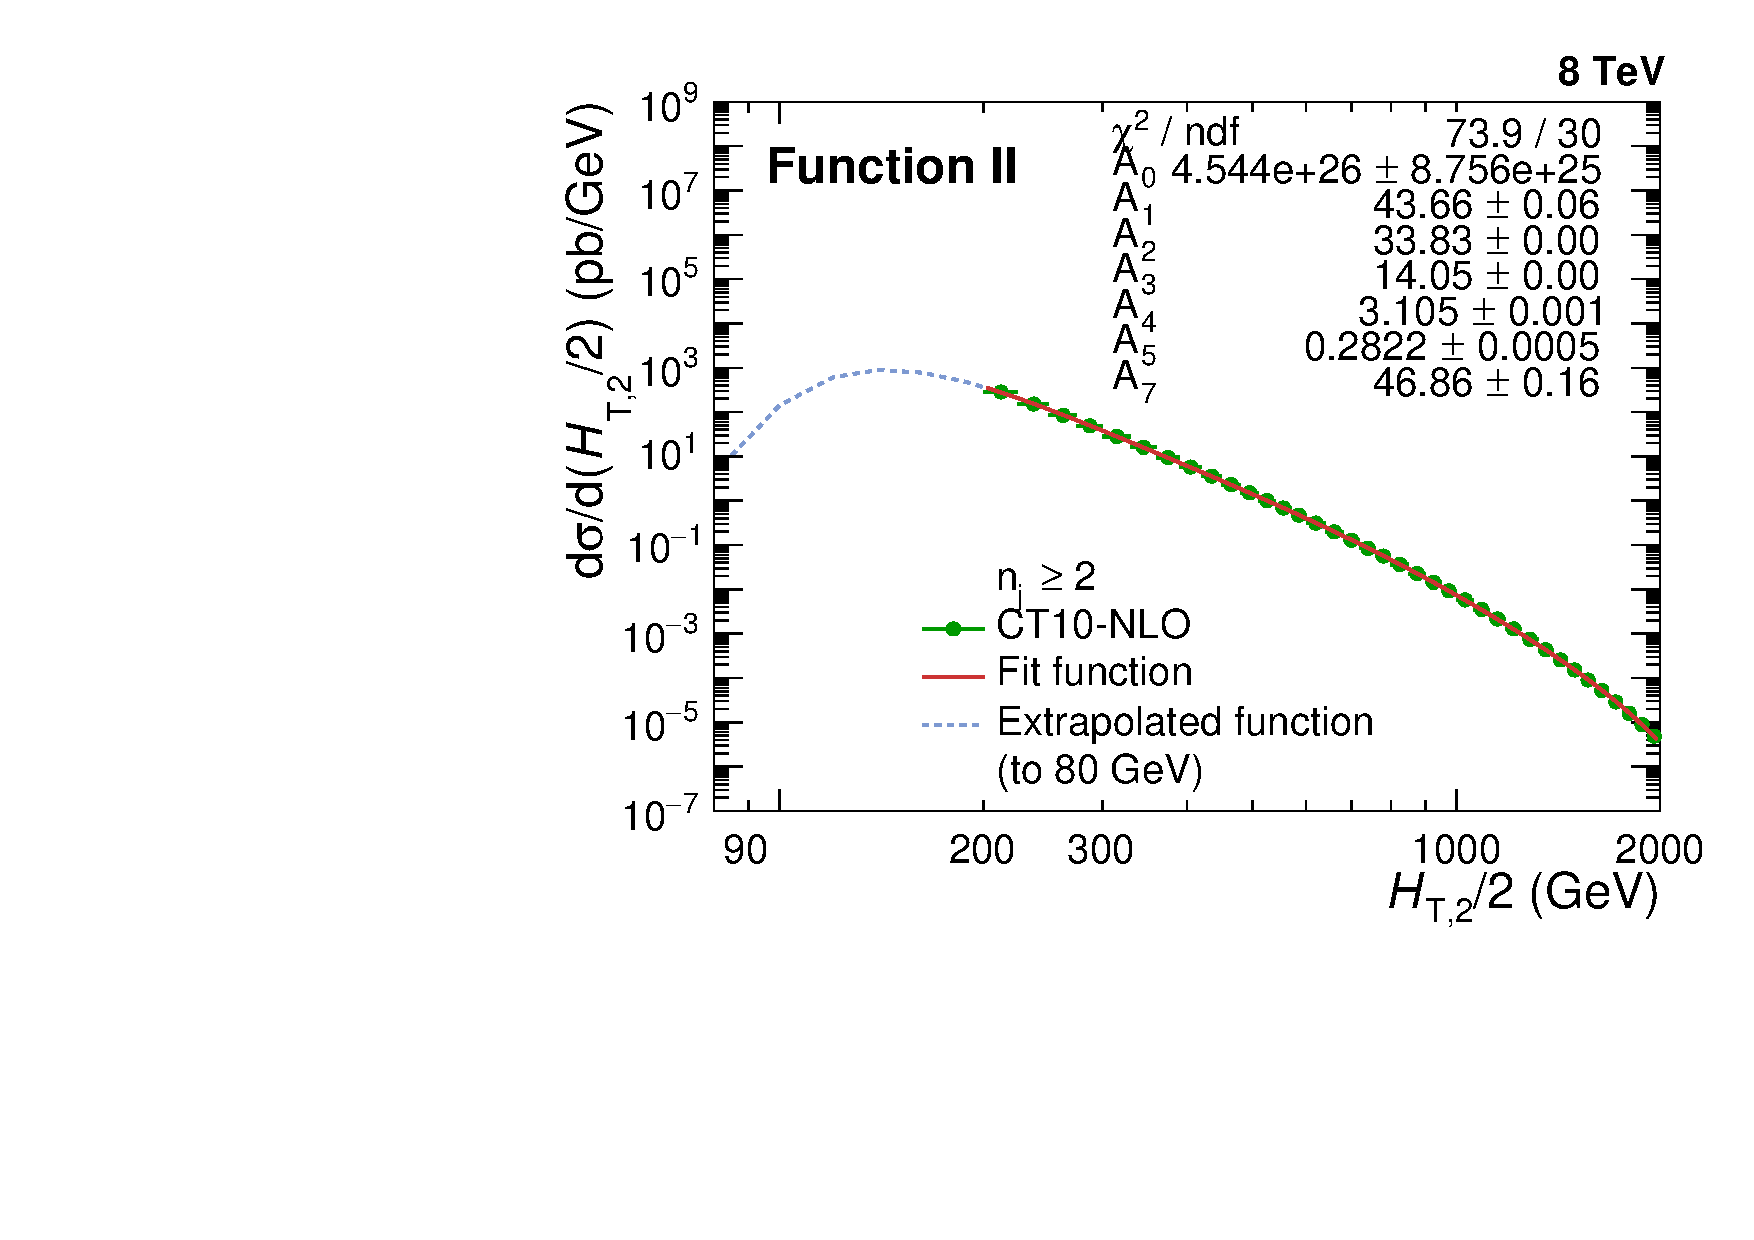
\includegraphics[width=0.51\textwidth]{Plots_HT_2_150/Extrapolate_Theory_2_HT_2_150_funcII.pdf}%
    ~~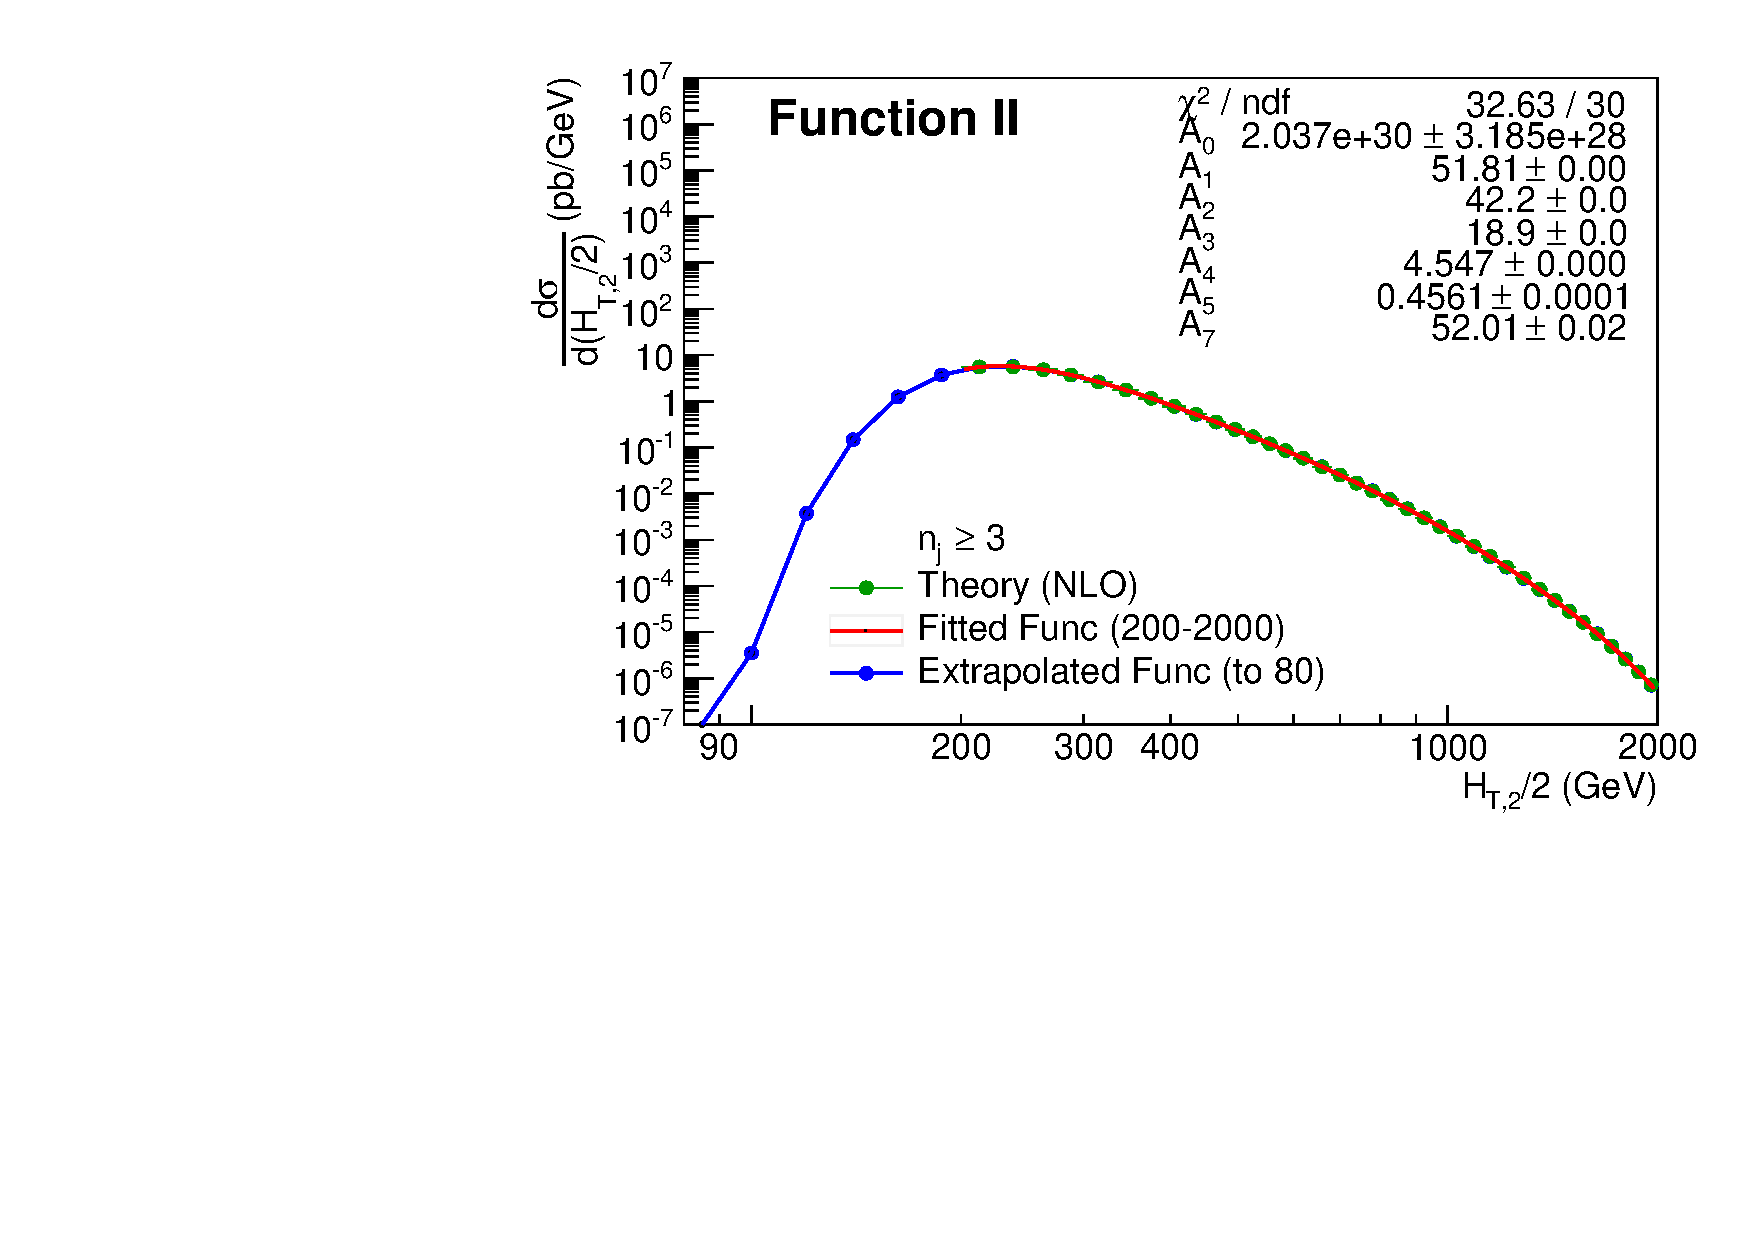
\includegraphics[width=0.51\textwidth]{Plots_HT_2_150/Extrapolate_Theory_3_HT_2_150_funcII.pdf}
    \caption[Fitted CT10-NLO spectrum of differential cross-section as a function of \httwo.]{Fitted CT10-NLO spectrum of differential cross-section as a function of \httwo (green solid circles) using Function I (top) defined in Eq.~\ref{eq:func1} and using Function II (bottom) given by Eq.~\ref{eq:func2}, for inclusive 2-jet (left) and 3-jet events (right). To consider the migration to lower \httwo bins, the fit functions described by red lines are extrapolated to 80 GeV (blue dashed lines).}
    \label{fig:fit}
  \end{center}
\end{figure}

Figure~\ref{fig:fit} shows the fitted CT10-NLO spectrum of differential cross-section as a function of \httwo (green solid circles) using Function I (top) and using Function II (bottom) : for inclusive 2-jet (left) and 3-jet events (right). Function I is used primarily to generate response matrices and perform the closure tests and Function II is used as an alternative function to calculate unfolding uncertainty, described in Sec.~\ref{sec:unfolding_unc}. To include the migration to lower bins, the fit functions described by red lines are extrapolated to 80 GeV (blue dashed lines).

A flat \httwo spectrum is generated by using toy Monte Carlo events and the fit parameters obtained from the NLO spectrum using function I (as shown in Fig.~\ref{fig:fit}) provides weights to the flat spectrum. A total of ten million events are generated randomly (in \httwo range 80-2000). These generated values are then smeared with a Gaussian function, where $\sigma$ of the Gaussian is determined from the relative resolution parametrization as a function of \httwo calculated from NSC formula mentioned in equation~\ref{NSC_formula}. The parameters N, S, C used for smearing are taken from Table~\ref{fit_para}. These randomly generated (Gen$_{\rm Toy}$) and smeared (Measured$_{\rm Toy}$) values are used to fill the response matrices. Figure~\ref{fig:response_NLO} shows the response matrices derived using the Toy MC for \njt~(left) and \njth~events (right). The matrices are normalized to the number of events in each column. The response matrices are diagonal as the migrations in off-diagonal bins are much smaller than the bins along the diagonal.

\begin{figure}[!htbp]
 \begin{center}
 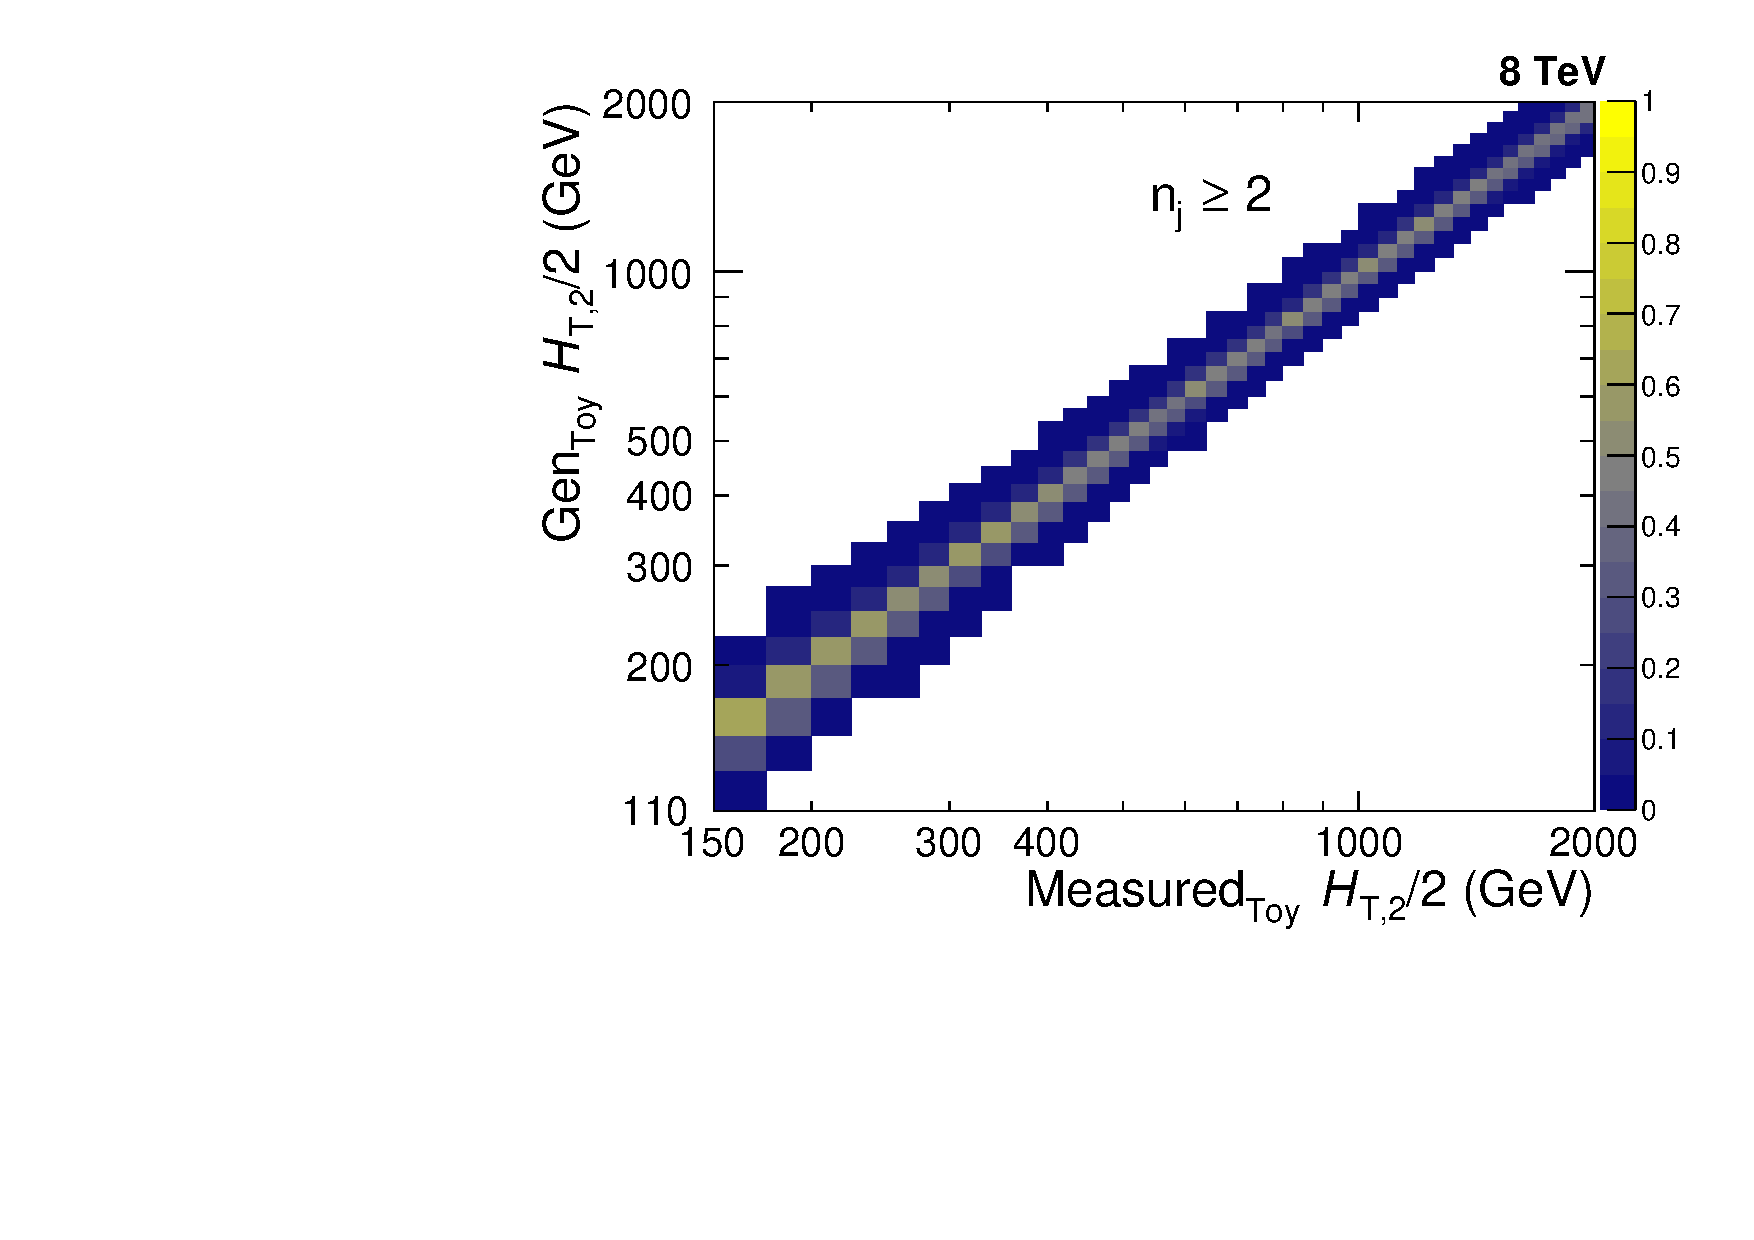
\includegraphics[width=0.51\textwidth]{Plots_HT_2_150/Normalized_Response_Matrix_NLO_2_range_column.pdf}%
 ~~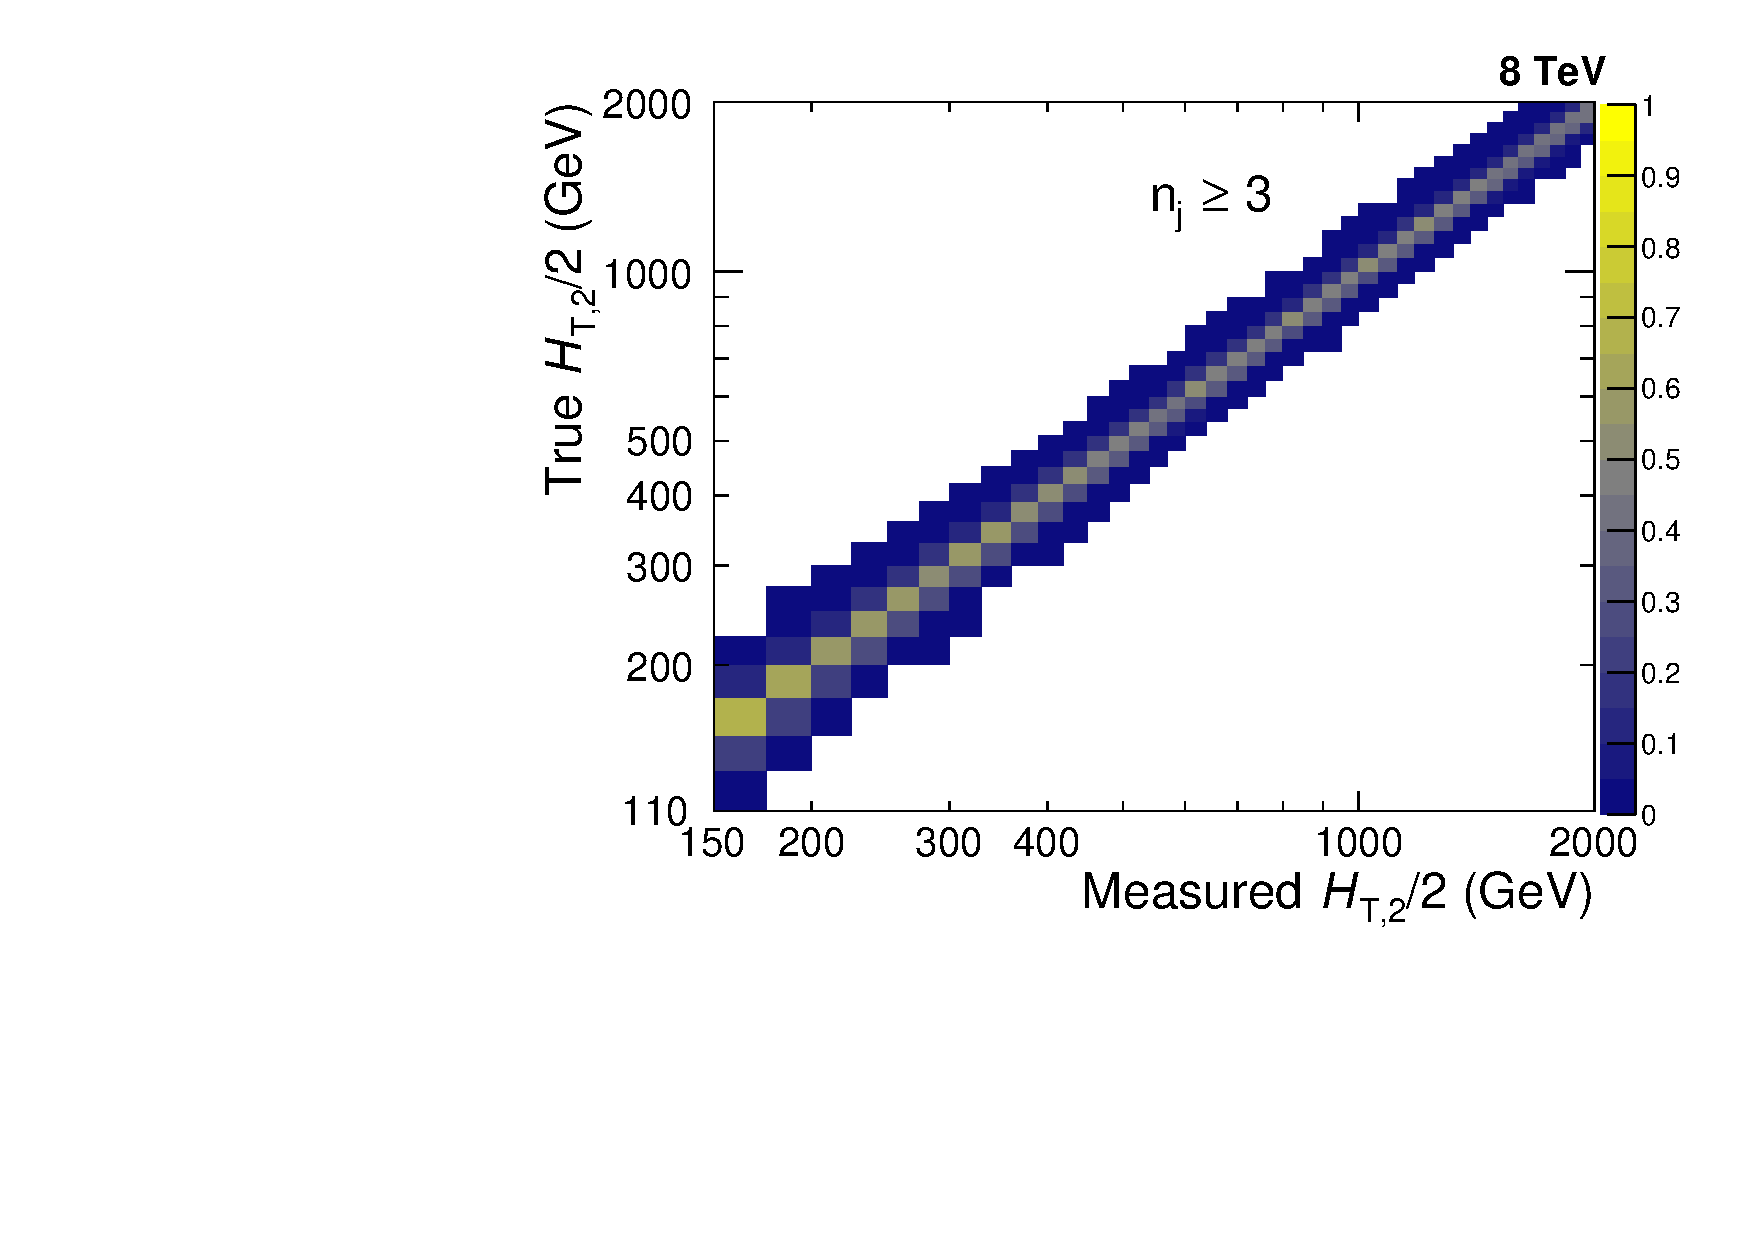
\includegraphics[width=0.51\textwidth]{Plots_HT_2_150/Normalized_Response_Matrix_NLO_3_column.pdf} 
 \caption[The response matrices are derived using the Toy Monte Carlo and forward smearing method.]{The response matrices are derived using the Toy Monte Carlo and forward smearing method, for inclusive 2-jet (left) and 3-jet events (right). The matrices are normalized to the number of events in each column and are diagonal with small off-diagonal migrations between close-by \httwo bins.}
 \label{fig:response_NLO}
 \end{center}
\end{figure}

\subsubsection{Cross-section Ratio, \texorpdfstring{\ratio}{R-32)}}
To obtain the statistical uncertainty on the unfolded cross-section ratio \rations, Method II is used. In this method, the response matrix is constructed using Toy MC method as done in Sec.~\ref{sec:cross_sec_res} for differential cross-sections. To obtain the true spectrum for \rations, the ratio of cross-section spectrum described by Eq.~\ref{eq:func1} for inclusive 3-jet to that of 2-jet events is taken. This ratio is shown by green solid circles in Fig.~\ref{fig:ratio_fit} (left) which is fitted using a polynomial function of degree 8 (red line). Then as explained in above section, response matrix is derived for \ratio using the Toy Monte Carlo and forward smearing method which is shown in Fig.~\ref{fig:ratio_fit} (right). The matrix is normalized to the number of events in each column and is diagonal with small off-diagonal migrations between close-by \httwo bins.

\begin{figure}[!htbp]
 \begin{center}
 \hspace*{-5mm}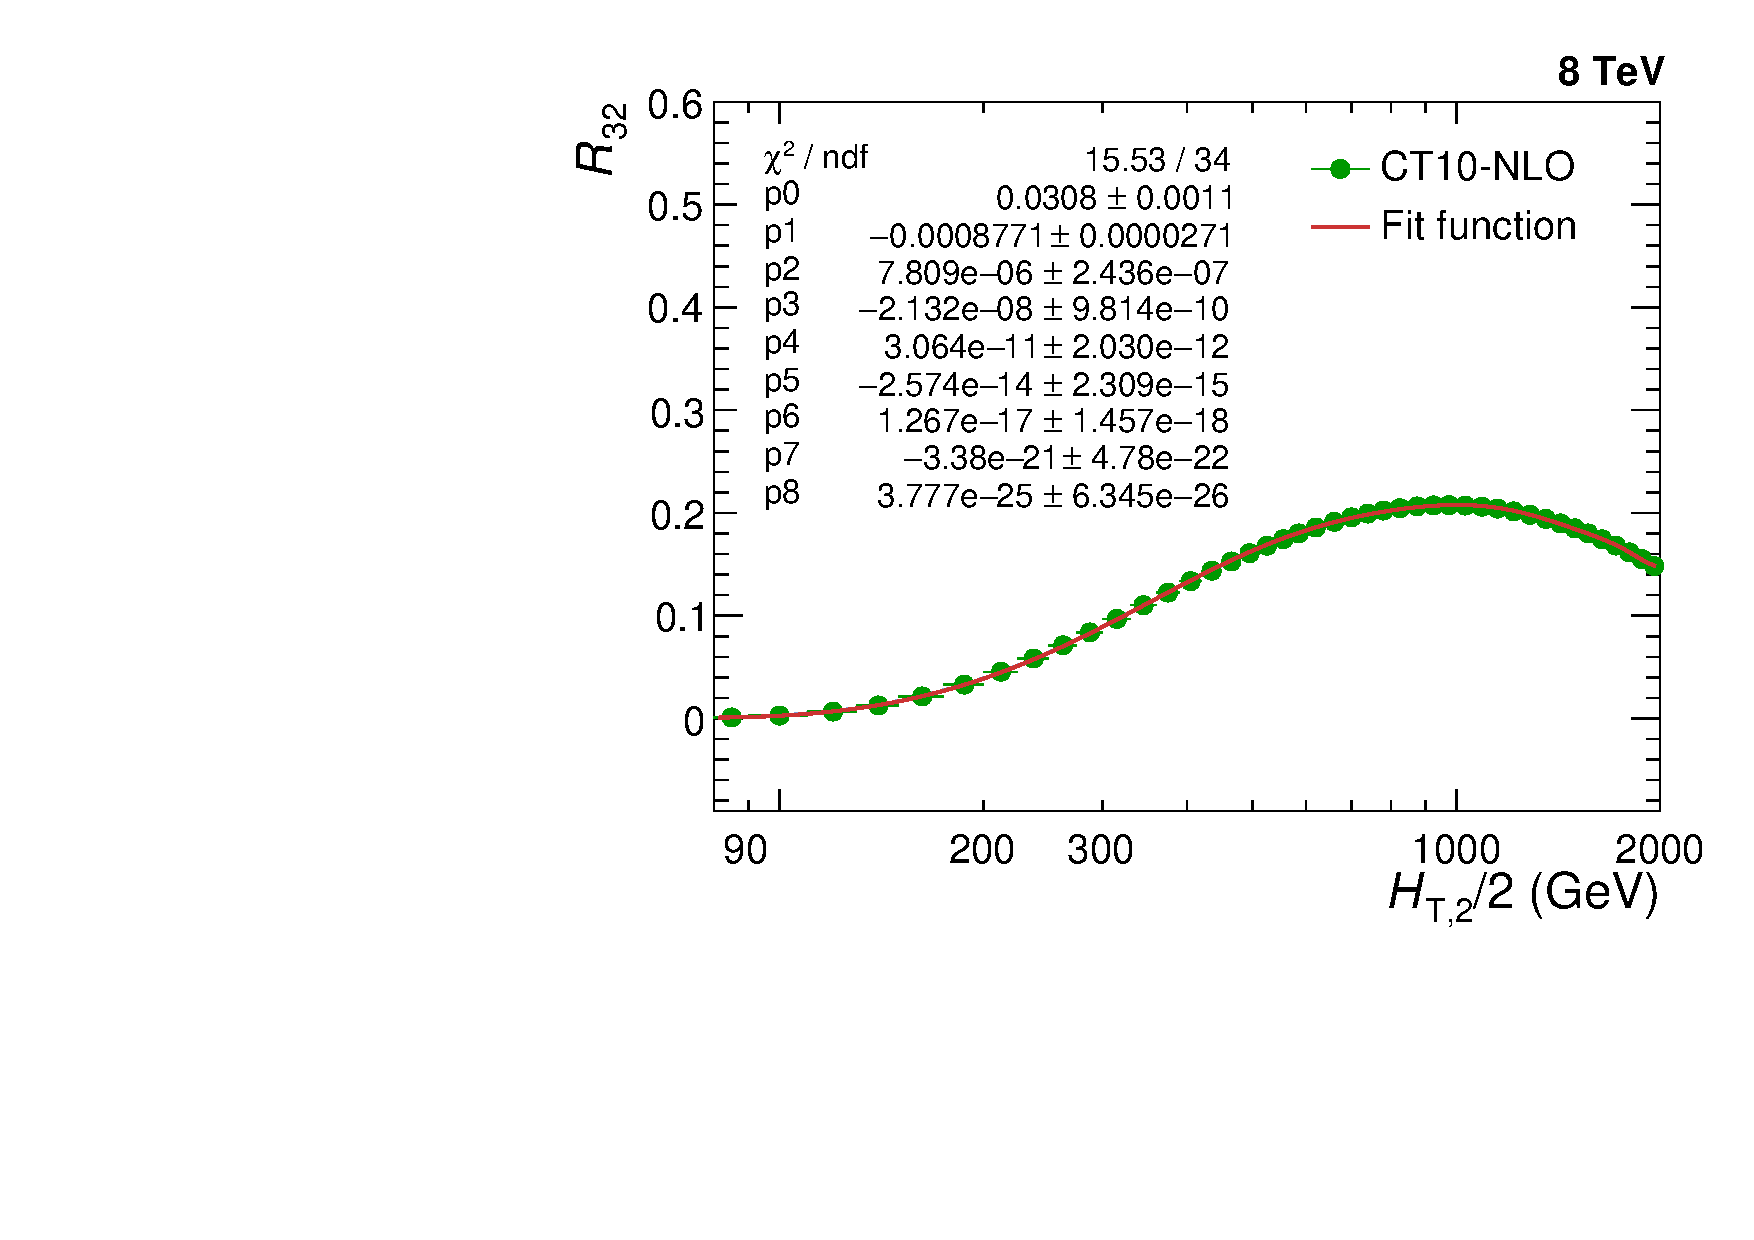
\includegraphics[width=0.51\textwidth]{Plots_HT_2_150/Extrapolate_Theory_Ratio_32_funcII.pdf}%
 ~~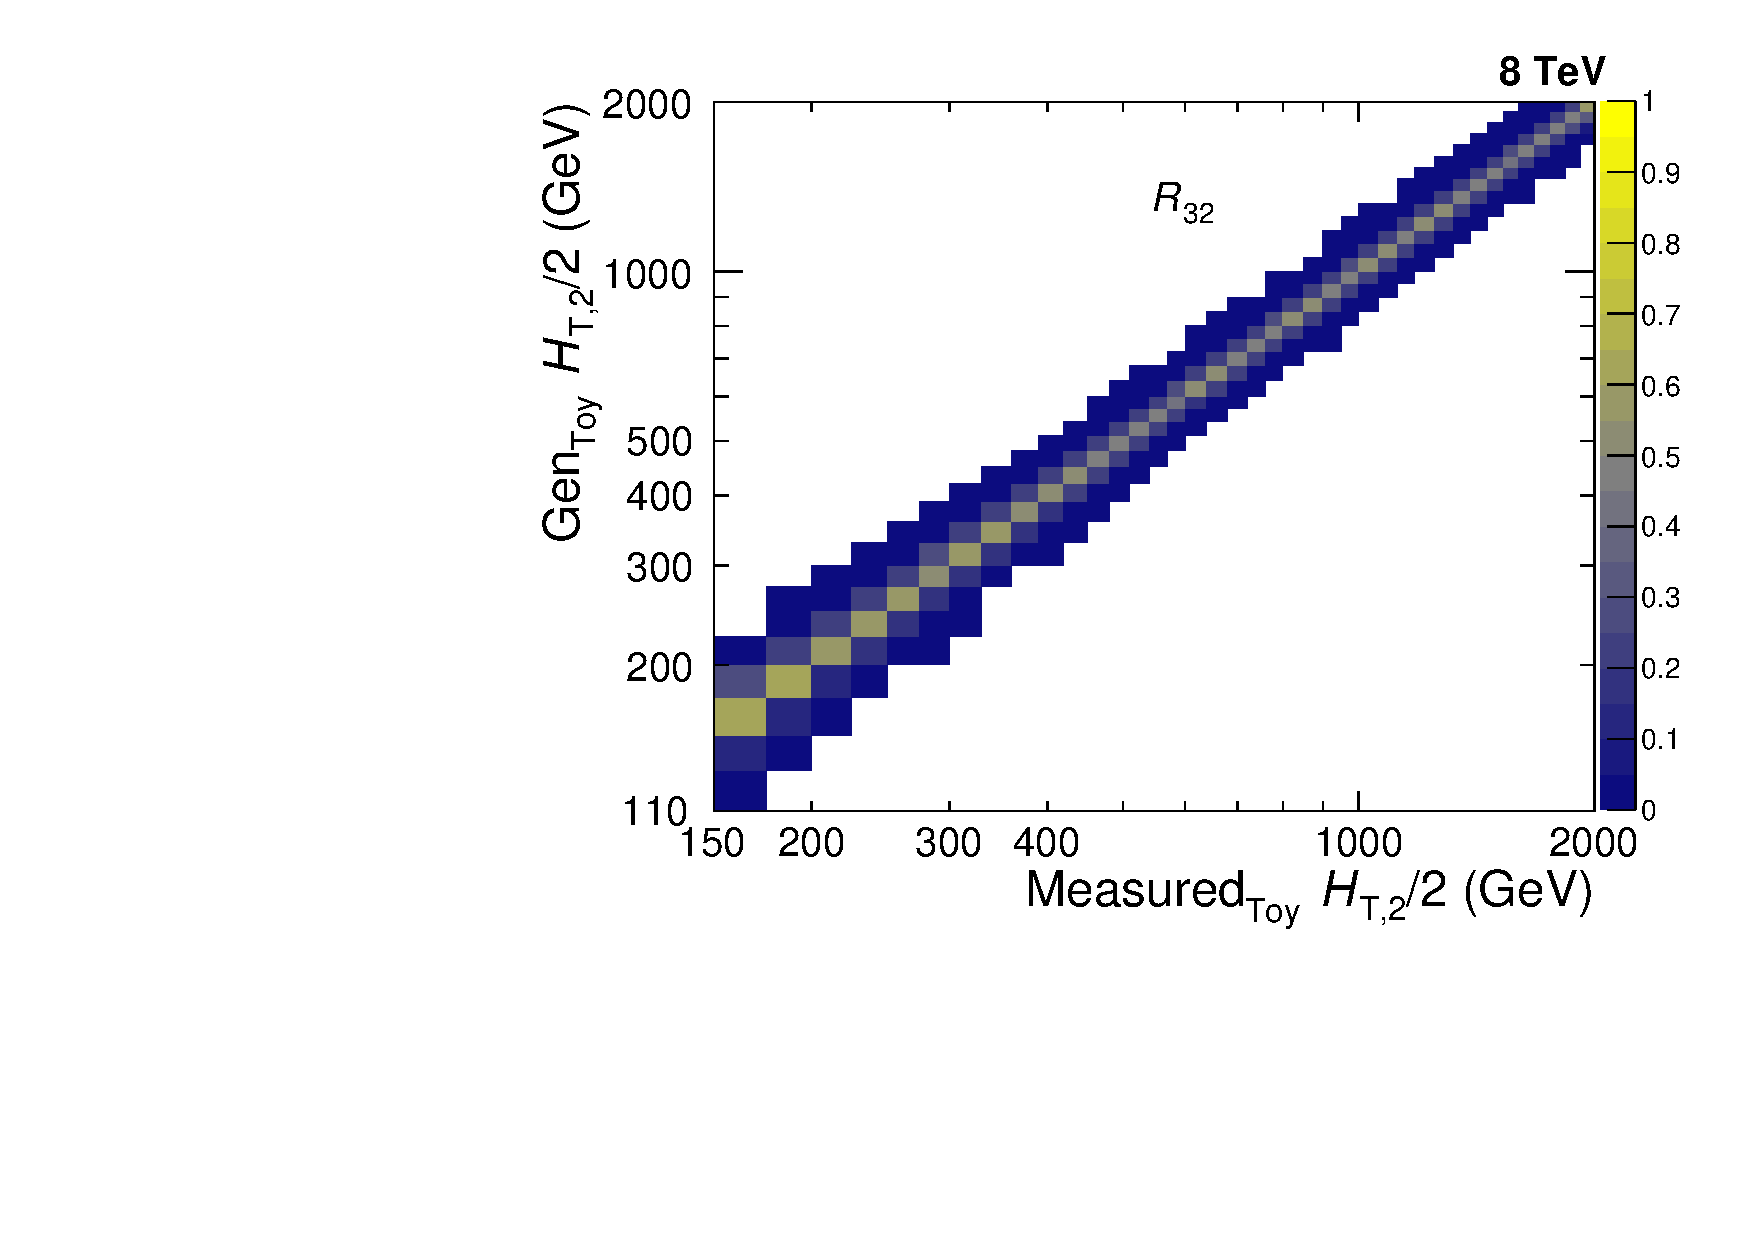
\includegraphics[width=0.51\textwidth]{Plots_HT_2_150/Normalized_Response_Matrix_NLO_ratio_32_column_3.pdf}
 \caption[Left : The ratio of cross-sections for inclusive 3-jet to that of 2-jet events as a function of \httwo. Right : The response matrix is derived using the Toy Monte Carlo and forward smearing method, for the cross-section ratio \rations.]{Left : The ratio of cross-sections described by Eq.~\ref{eq:func1} for inclusive 3-jet to that of 2-jet events is shown as a function of \httwo (green solid circles). It is fit using a polynomial function of degree 8 (red line). Right : The response matrix is derived using the Toy Monte Carlo and forward smearing method, for the cross-section ratio \rations. The matrix is normalized to the number of events in each column and is diagonal with small off-diagonal migrations between close-by \httwo bins.}
 \label{fig:ratio_fit}
 \end{center}
\end{figure}

\subsection{Closure Test}
A closure test has been performed to confirm the working of the unfolding procedure. In this test, Measured$_{\rm Toy}$ spectrum is unfolded using the constructed response matrices shown in Figure~\ref{fig:response_NLO}. It is expected that the same Gen$_{\rm Toy}$ spectrum should be re-obtained after unfolding. Figure~\ref{fig:unfolded_smeared} confirms that the unfolded Measured$_{\rm Toy}$ spectrum matches exactly with Gen$_{\rm Toy}$ spectrum as the ratio of these distributions is perfectly flat at one for both \njt~(top left) and \njth~events (top right) cross-sections as well as the cross-section ratio \ratio (bottom).

\begin{figure}[!ht]
 \begin{center}
 \hspace*{-3mm}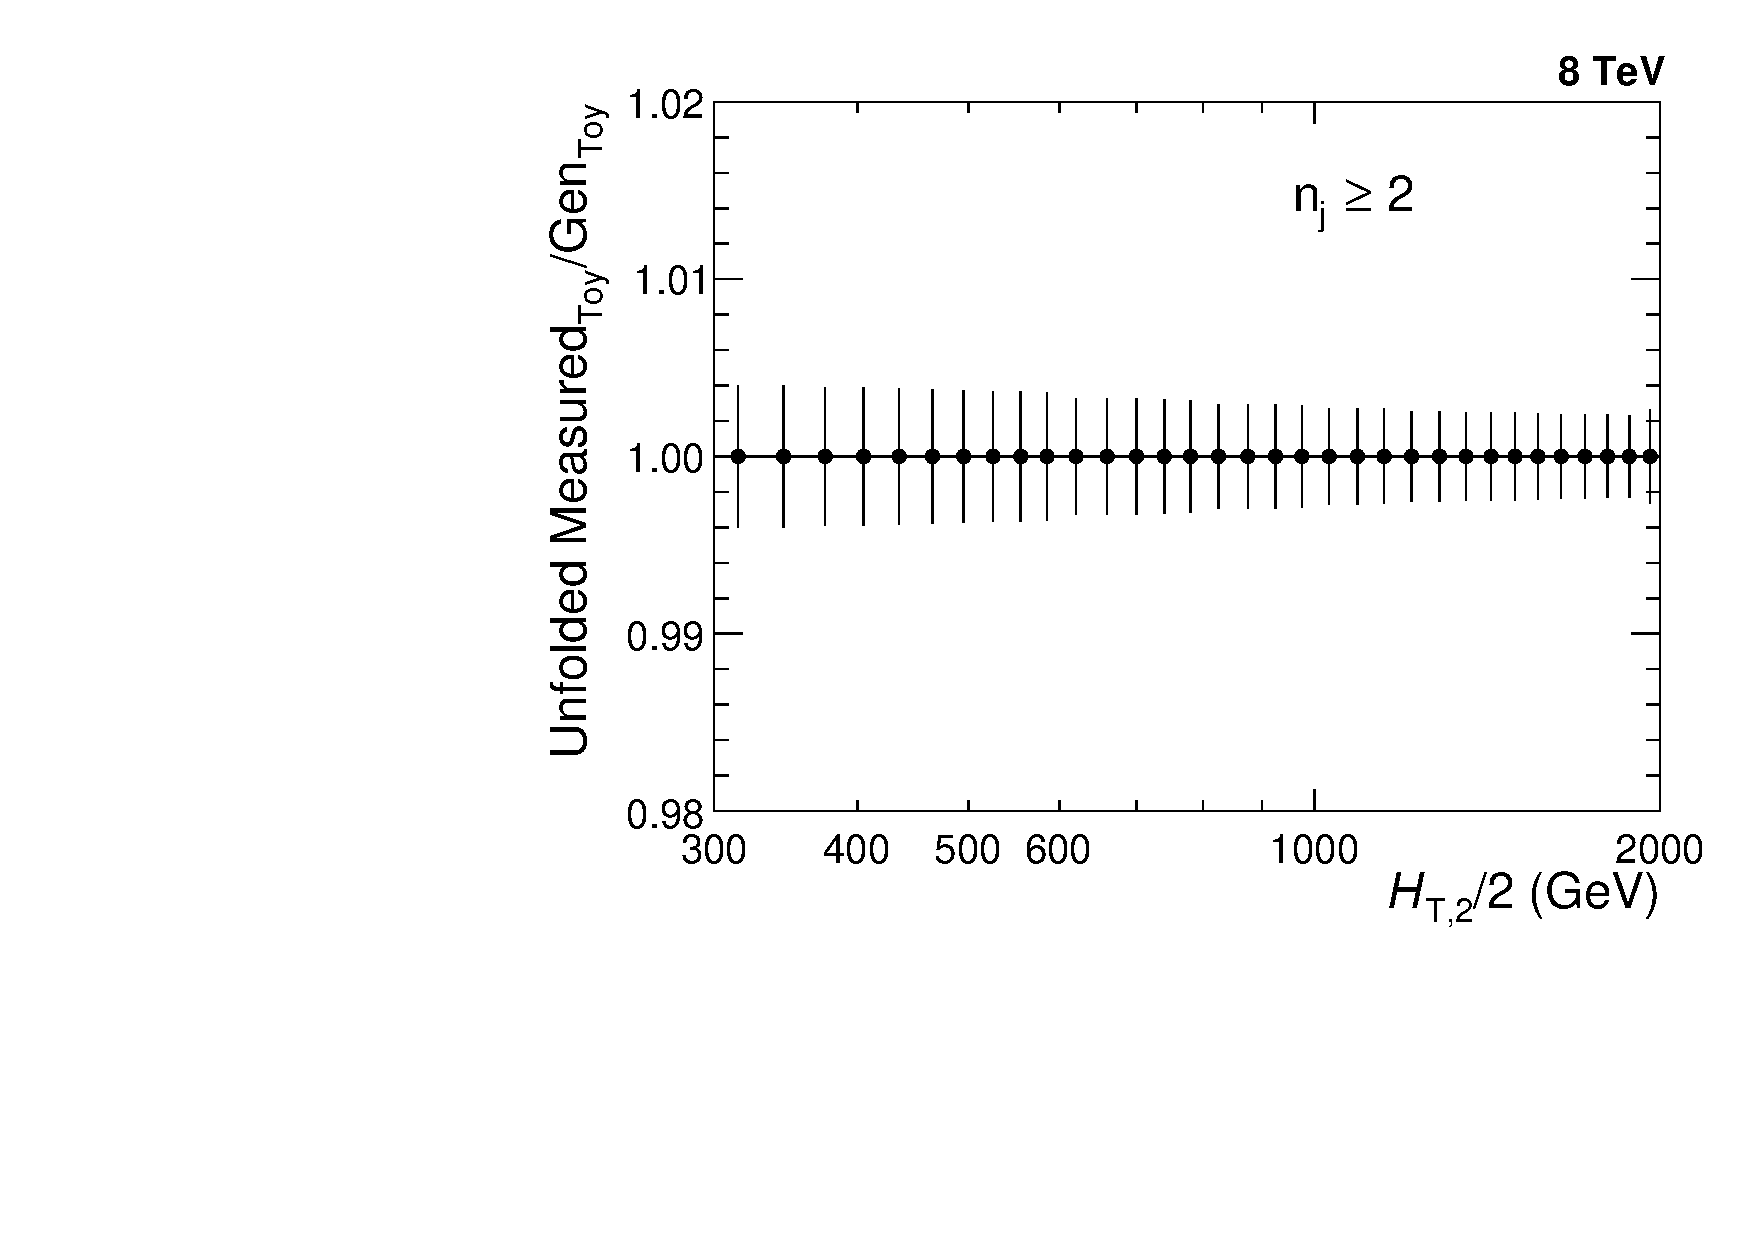
\includegraphics[width=0.51\textwidth]{Plots_HT_2_150/Ratio_Unfolding_NLO_2_funcI.pdf}%
 ~~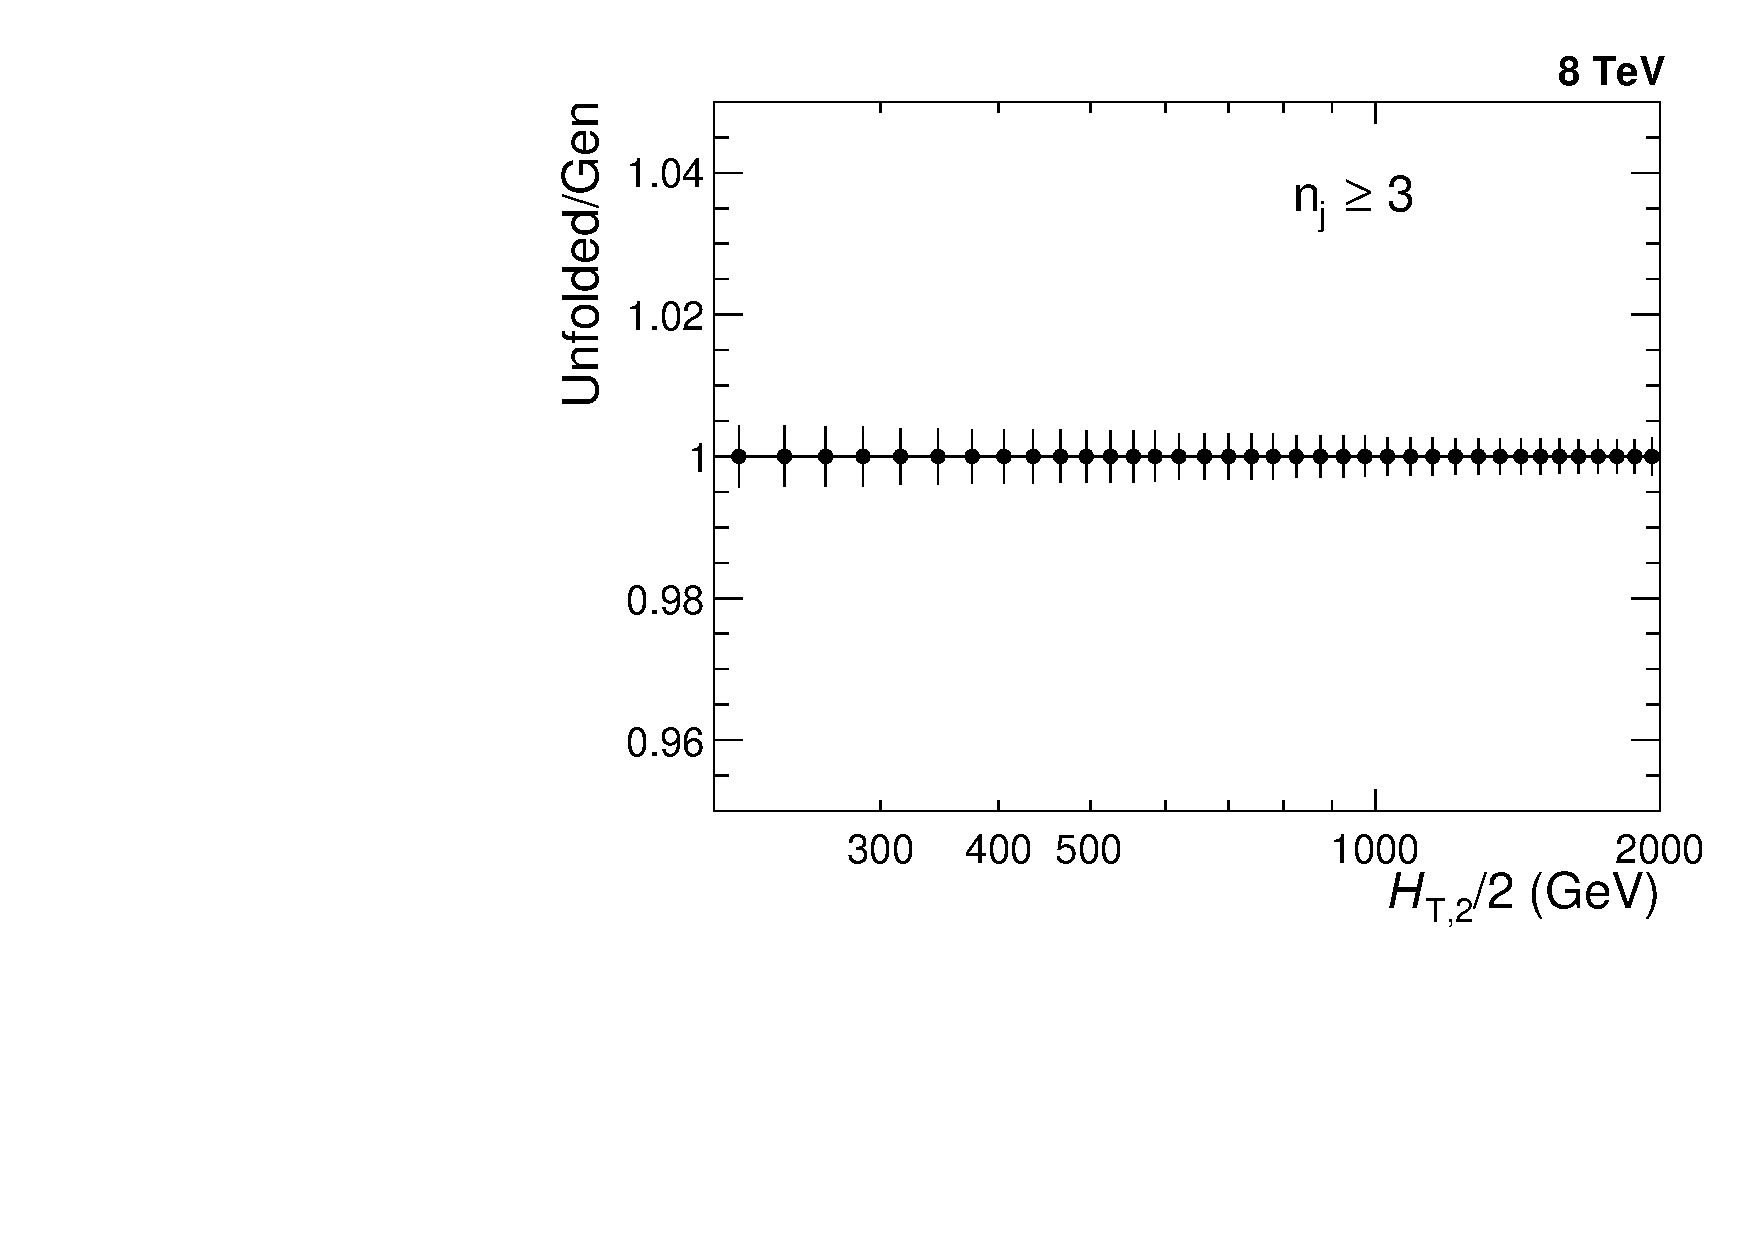
\includegraphics[width=0.51\textwidth]{Plots_HT_2_150/Ratio_Unfolding_NLO_3_funcI.pdf}\\
 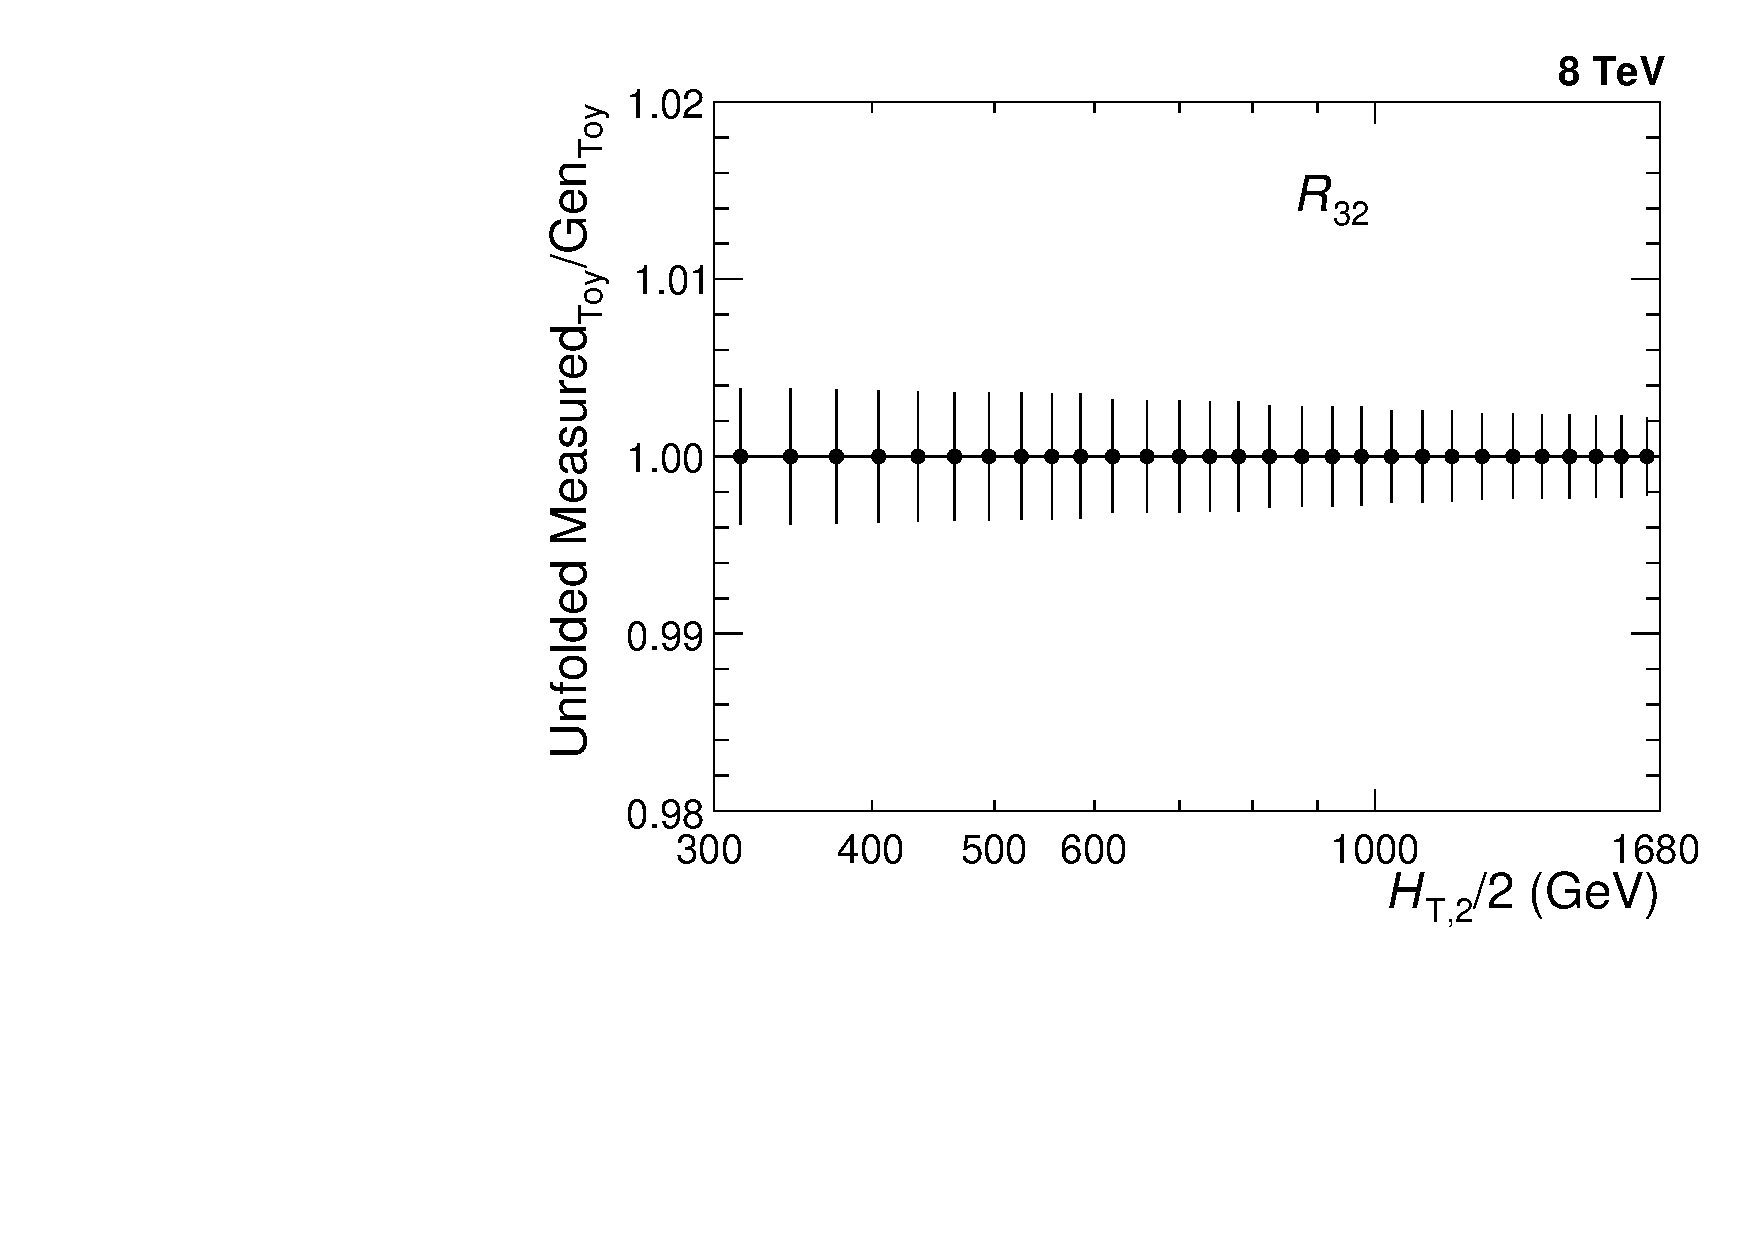
\includegraphics[width=0.51\textwidth]{Plots_HT_2_150/Ratio_Unfolding_NLO_Ratio_32_funcI.pdf}
 \caption[Closure test of the unfolding technique .]{Closure test of the unfolding technique where the smeared spectrum obtained from Toy Monte Carlo method (Measured$_{\rm Toy}$), is unfolded using the constructed response matrices (obtained by forward smearing the randomly generated spectrum (Gen$_{\rm Toy}$) using extracted jet energy resolution (JER)). As expected, the unfolded measured$_{\rm Toy}$ spectrum matches exactly with Gen$_{\rm Toy}$ spectrum as the ratio of these distributions is perfectly flat at one for both inclusive 2-jet (top left) and 3-jet events (top right) cross-sections as well as the cross-section ratio \ratio (bottom).}
 \label{fig:unfolded_smeared}
 \end{center}
\end{figure}

\begin{figure}[!h]
 \begin{center}
 \hspace*{-3mm}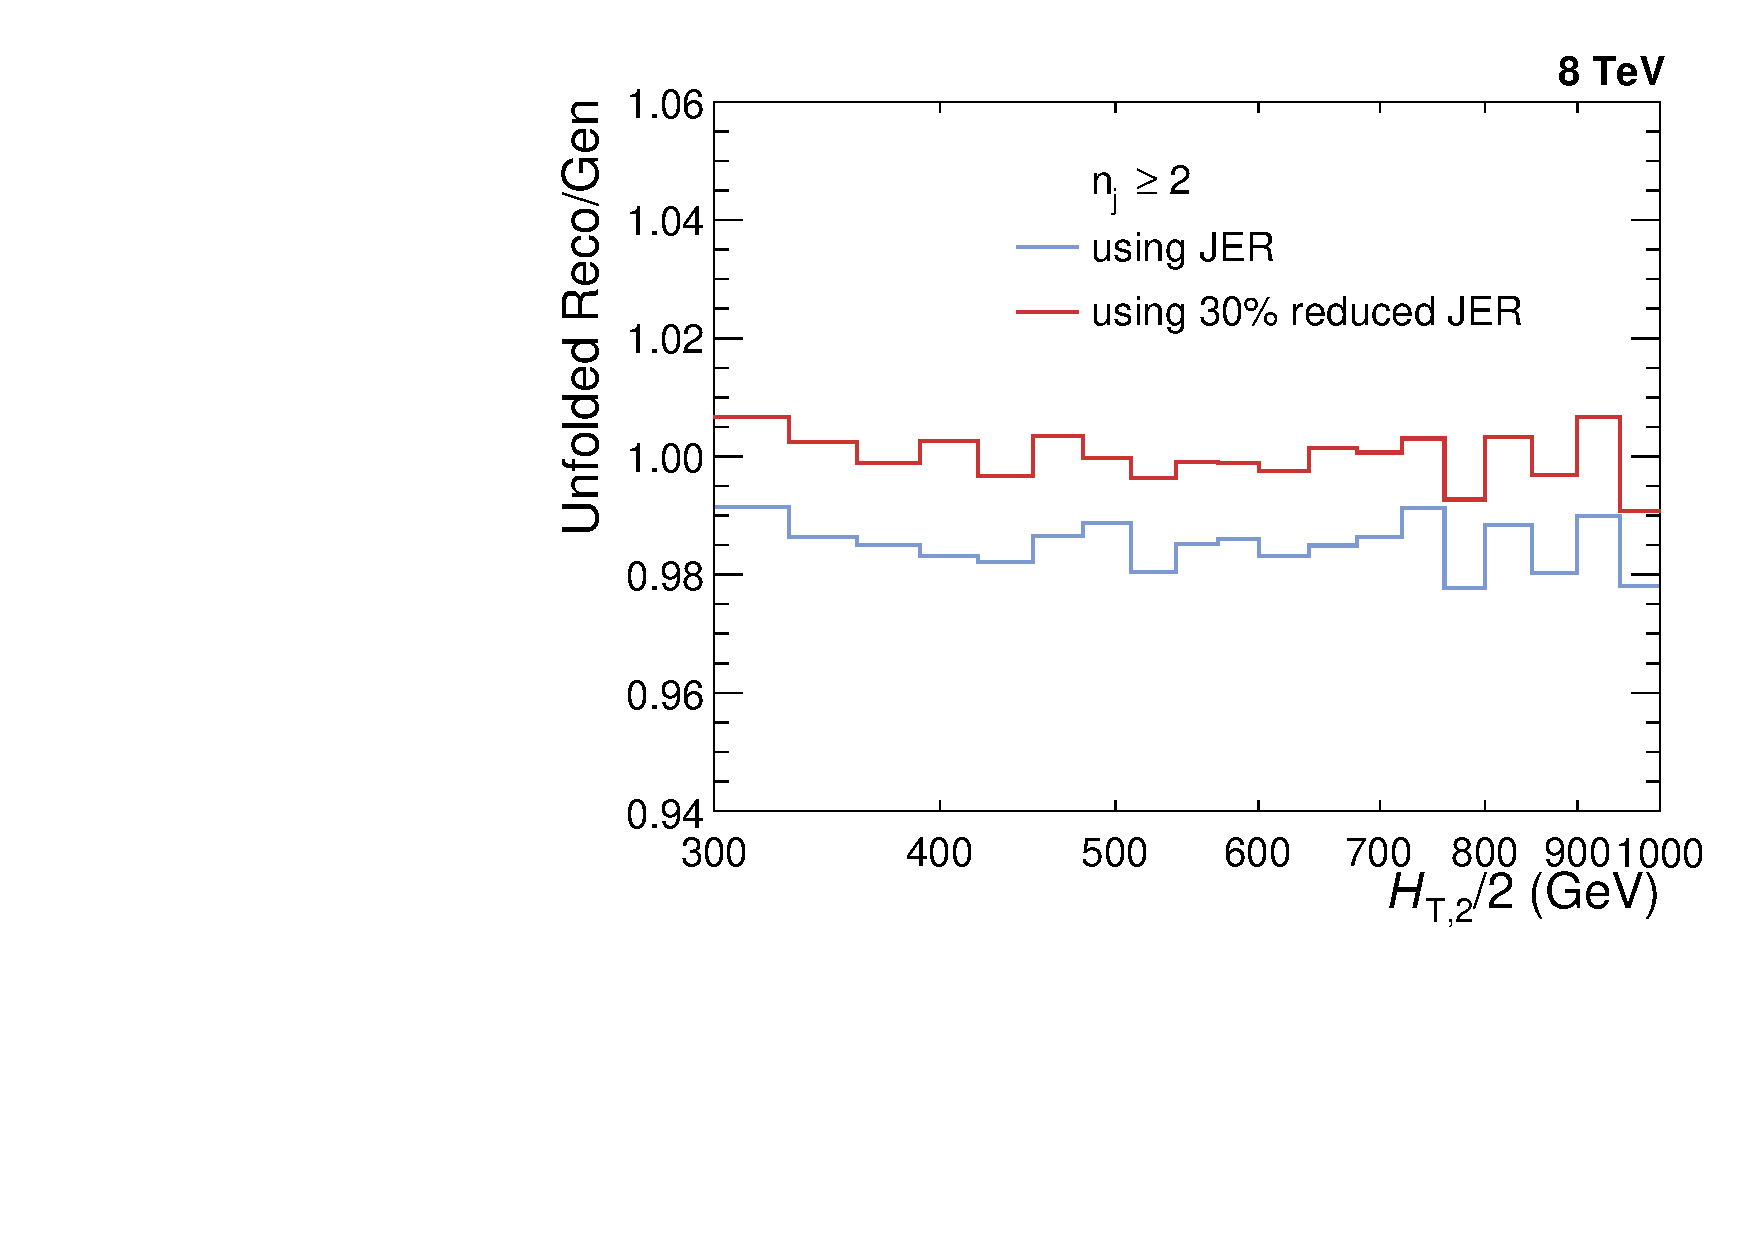
\includegraphics[width=0.51\textwidth]{Plots_HT_2_150/Comparison_closure_2_range.pdf}%
 ~~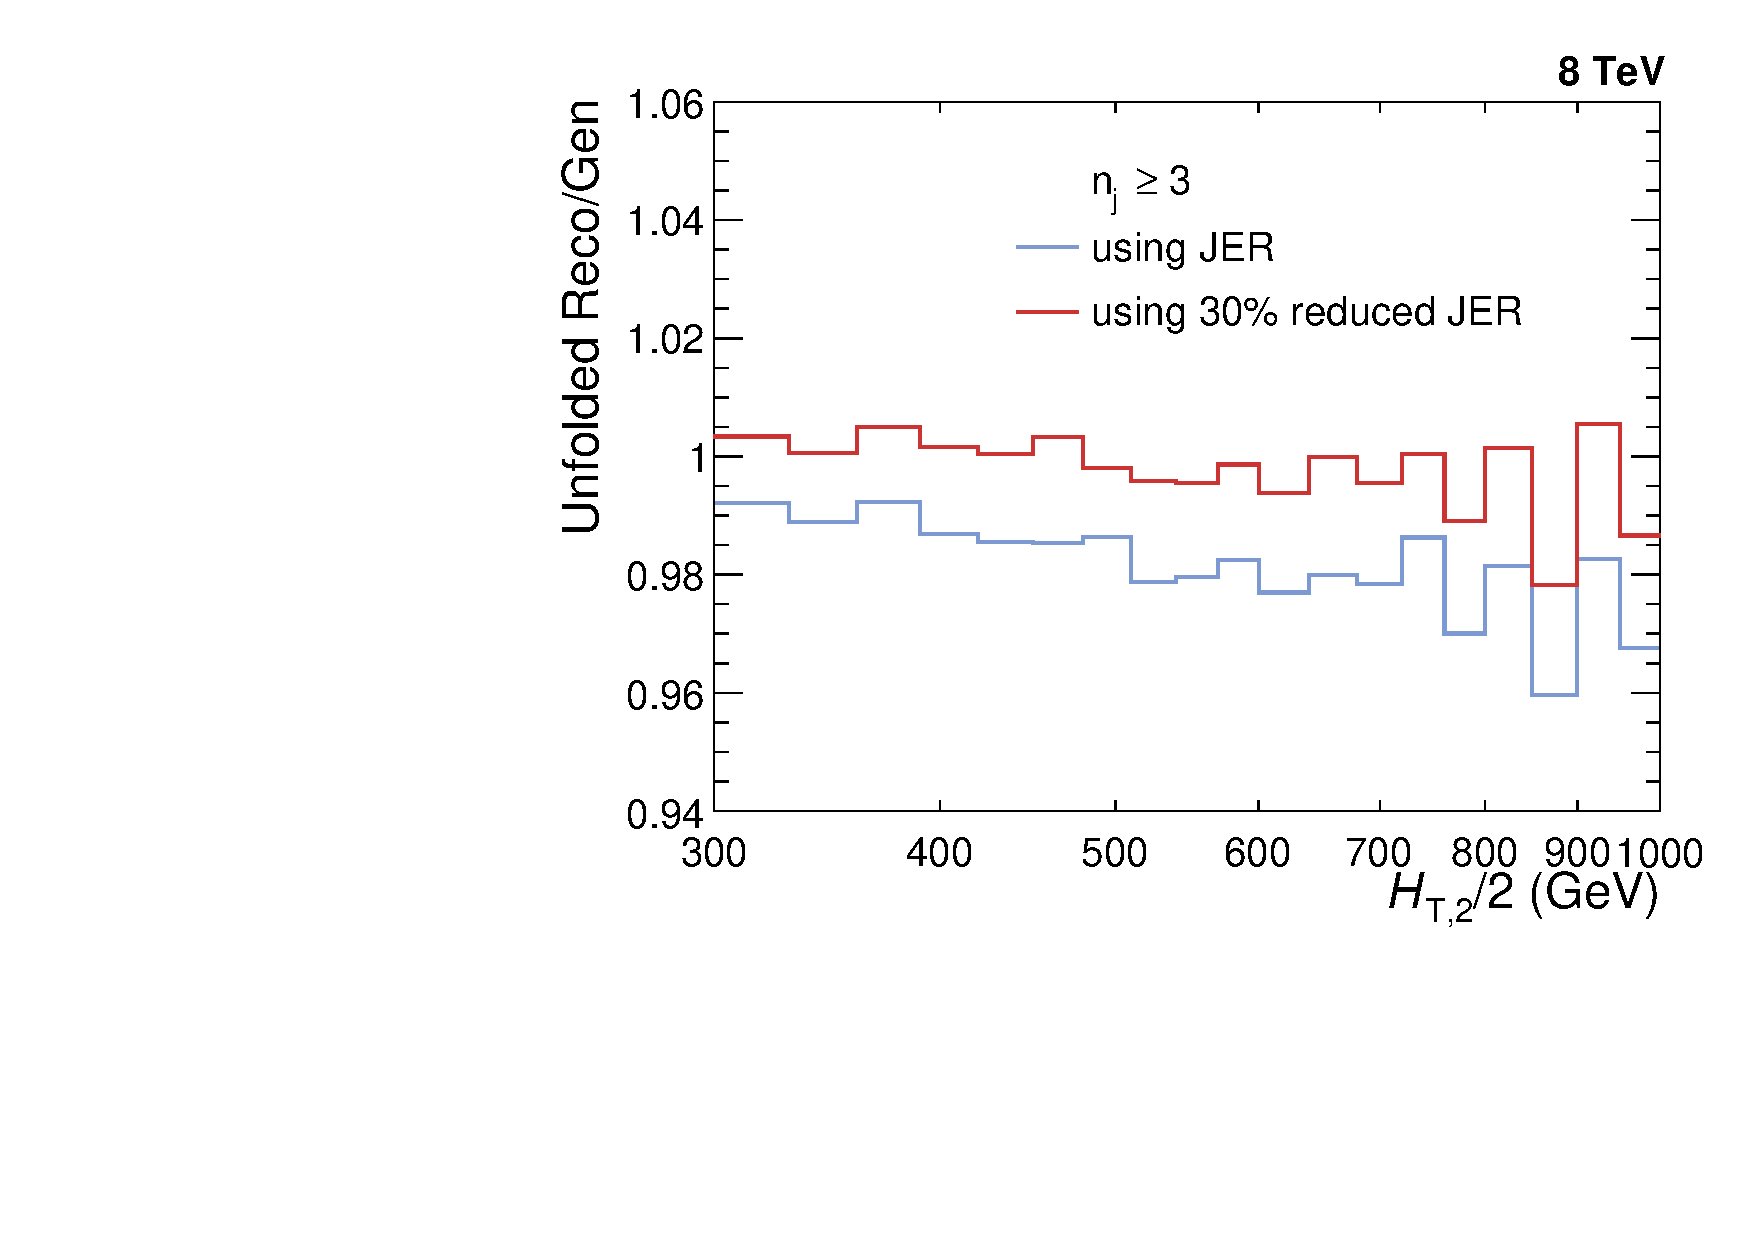
\includegraphics[width=0.51\textwidth]{Plots_HT_2_150/Comparison_closure_3.pdf}\\
 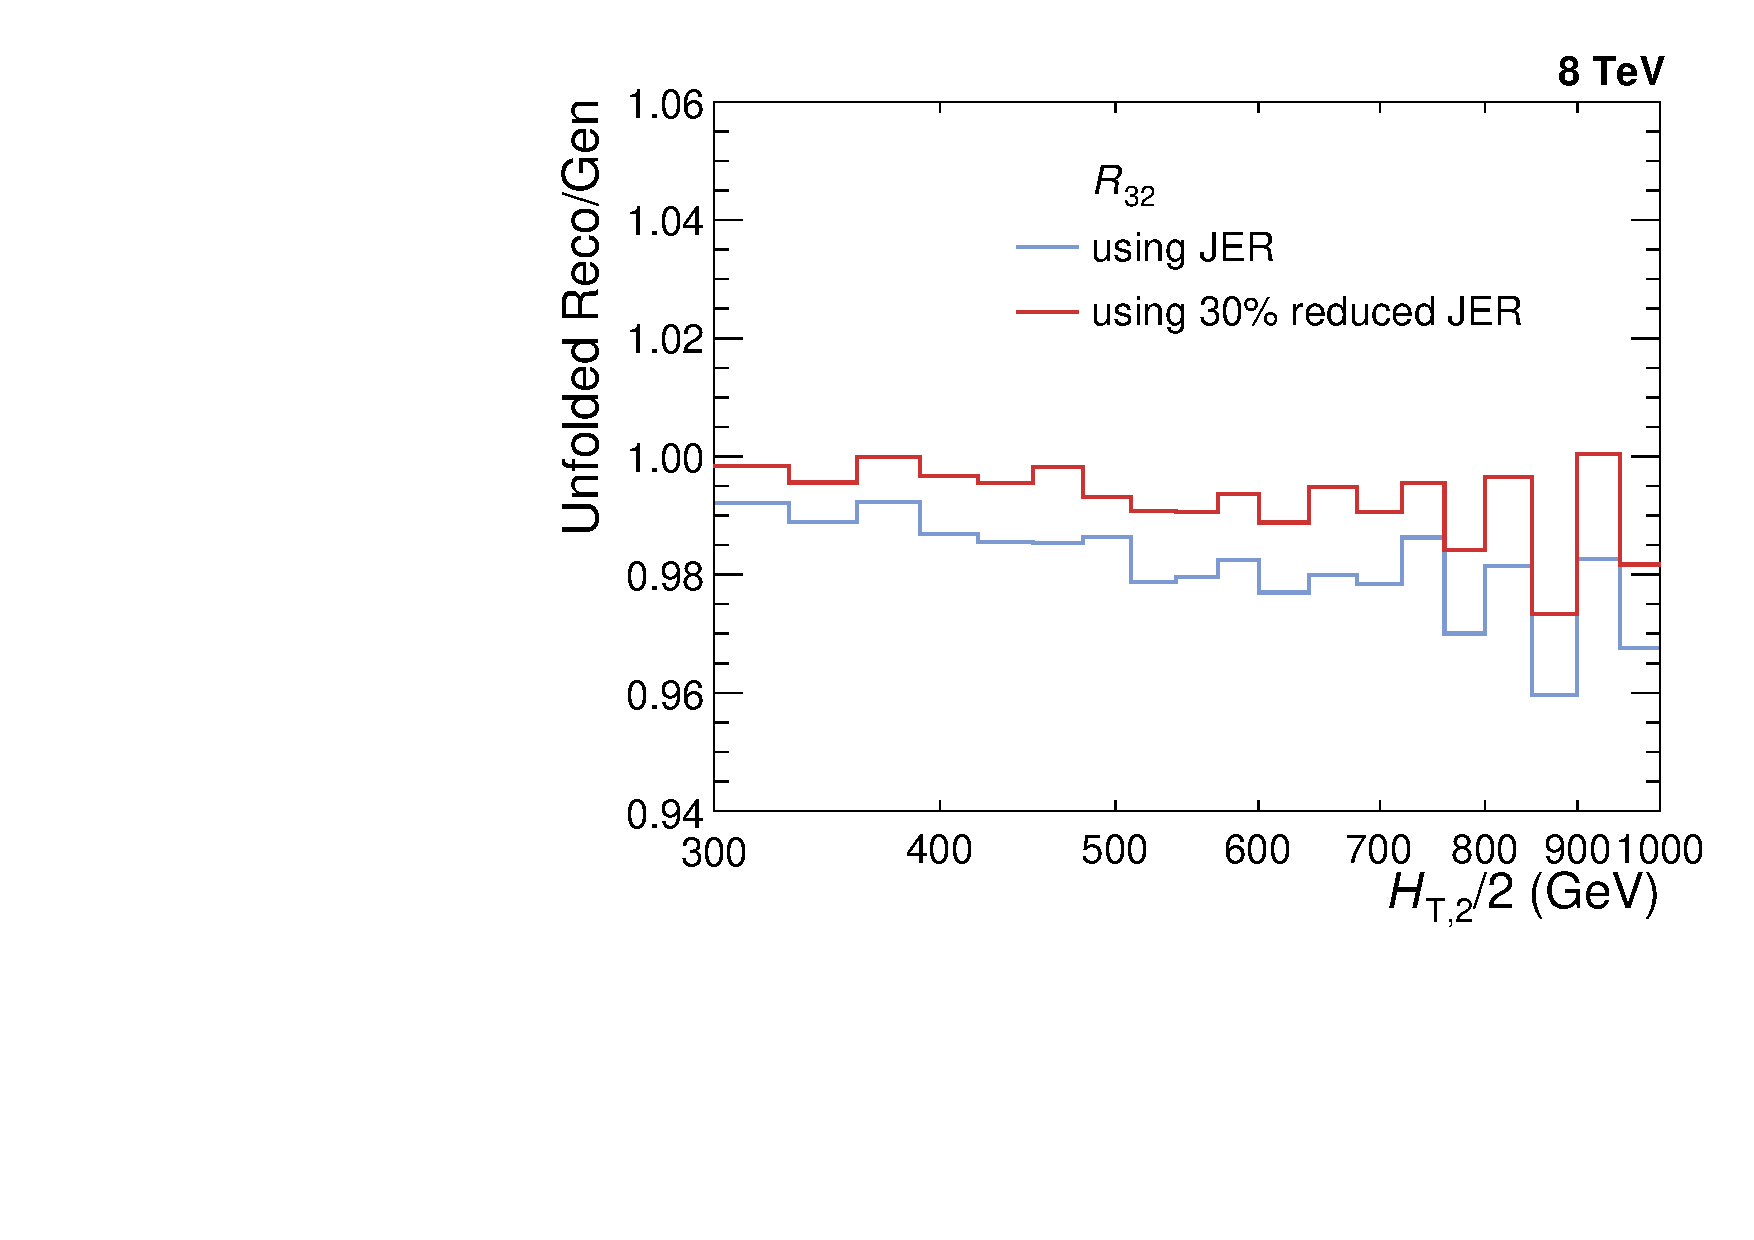
\includegraphics[width=0.51\textwidth]{Plots_HT_2_150/Comparison_closure_ratio_32_now.pdf}
 \caption[Reco differential cross-section distributions unfolded with the response matrices.]{Reco \MadGraphFn\plusn \PYTHIAS Monte Carlo (\MGP~MC) differential cross-section distributions unfolded with the response matrices (obtained by forward smearing the randomly generated spectrum (Gen) using extracted jet energy resolution (JER)), does not give a good closure with Gen \MGP~MC (blue line), for inclusive 2-jet (top left) and 3-jet events (top right). After performing the unfolding using 30\% reduced JER, a good closure is obtained (red line). Since unfolded the cross-section ratio \ratio is the ratio of unfolded differential cross-sections, same behaviour is observed for \ratio (bottom).}
 \label{fig:unfolded_reco_NLO}
 \end{center}
\end{figure}

For another closure test, Reco \MGP~MC differential cross-section distribution is unfolded using the above constructed response matrices using JER for forward smearing the randomly generated spectrum. While taking ratio of the unfolded distribution to that of Gen \MGP~MC, it is observed that a well closure is not obtained. This is represented by blue line in Fig.~\ref{fig:unfolded_reco_NLO} for \njt~(top left) and \njth~events (top right). As observed in Fig.~\ref{fig:ratios} in Sec.~\ref{sec:Resolution}, if Reco \MGP~MC is unfolded using the response matrices obtained using 30\% reduced JER, then the good closure is obtained as shown by red line in Fig.~\ref{fig:unfolded_reco_NLO}. Since unfolded cross-section ratio \ratio is the ratio of unfolded differential cross-sections (Method I), same behaviour is observed for \ratio (bottom). 

\subsection{Unfolding of the Measurement}
\label{subsec:unf}
After validity the unfolding method, the measured differential cross-sections as well as \ratio are unfolded using the above reconstructed response matrices. The unfolded data spectrum is compared to that of measured one in Fig.~\ref{fig:unfolded_data} for \njt~(top left) and \njth~events (top right) cross-sections and for the cross-section ratio \ratio (bottom). As already discussed that 30\% reduced JER gives better closures than JER, so the unfolding of data is done with response matrices using JER (blue solid circles) as well as 30\% reduced JER (red solid circles) for smearing. The difference between both is taken as an additional uncertainty on the unfolded measurement. %The unfolding does not working well for bins near to minimum \pt cut for inclusive 2-jet events because two-jet rate is very sensitive to soft gluon emission while the higher jet multiplicities are less affected. %The event yield for each bin in \httwo is tabulated in Appendix in Table~\ref{table_event}. 

\begin{figure}[!h]
 \begin{center}
 \hspace*{-3mm}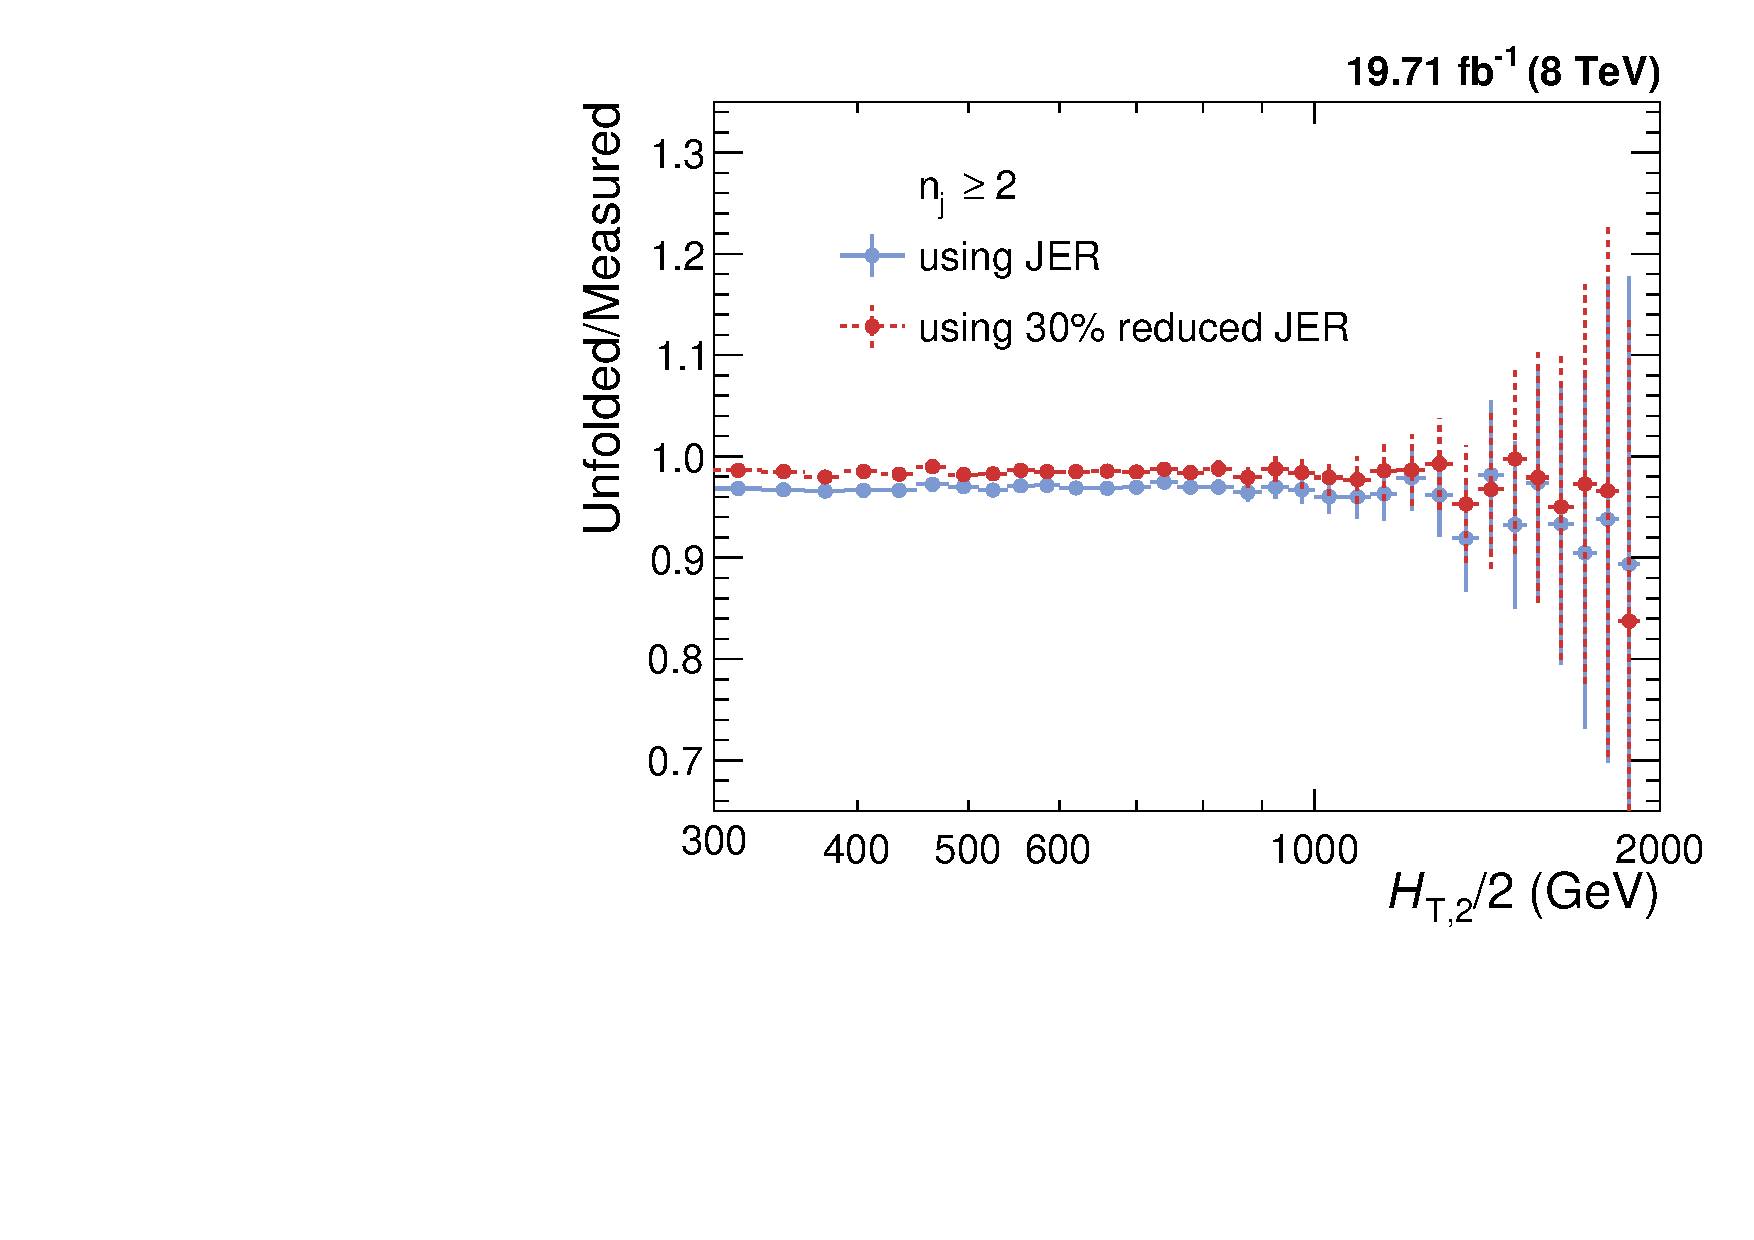
\includegraphics[width=0.51\textwidth]{Plots_HT_2_150/Ratio_Unfolding_data_NLO_2.pdf}%
 ~~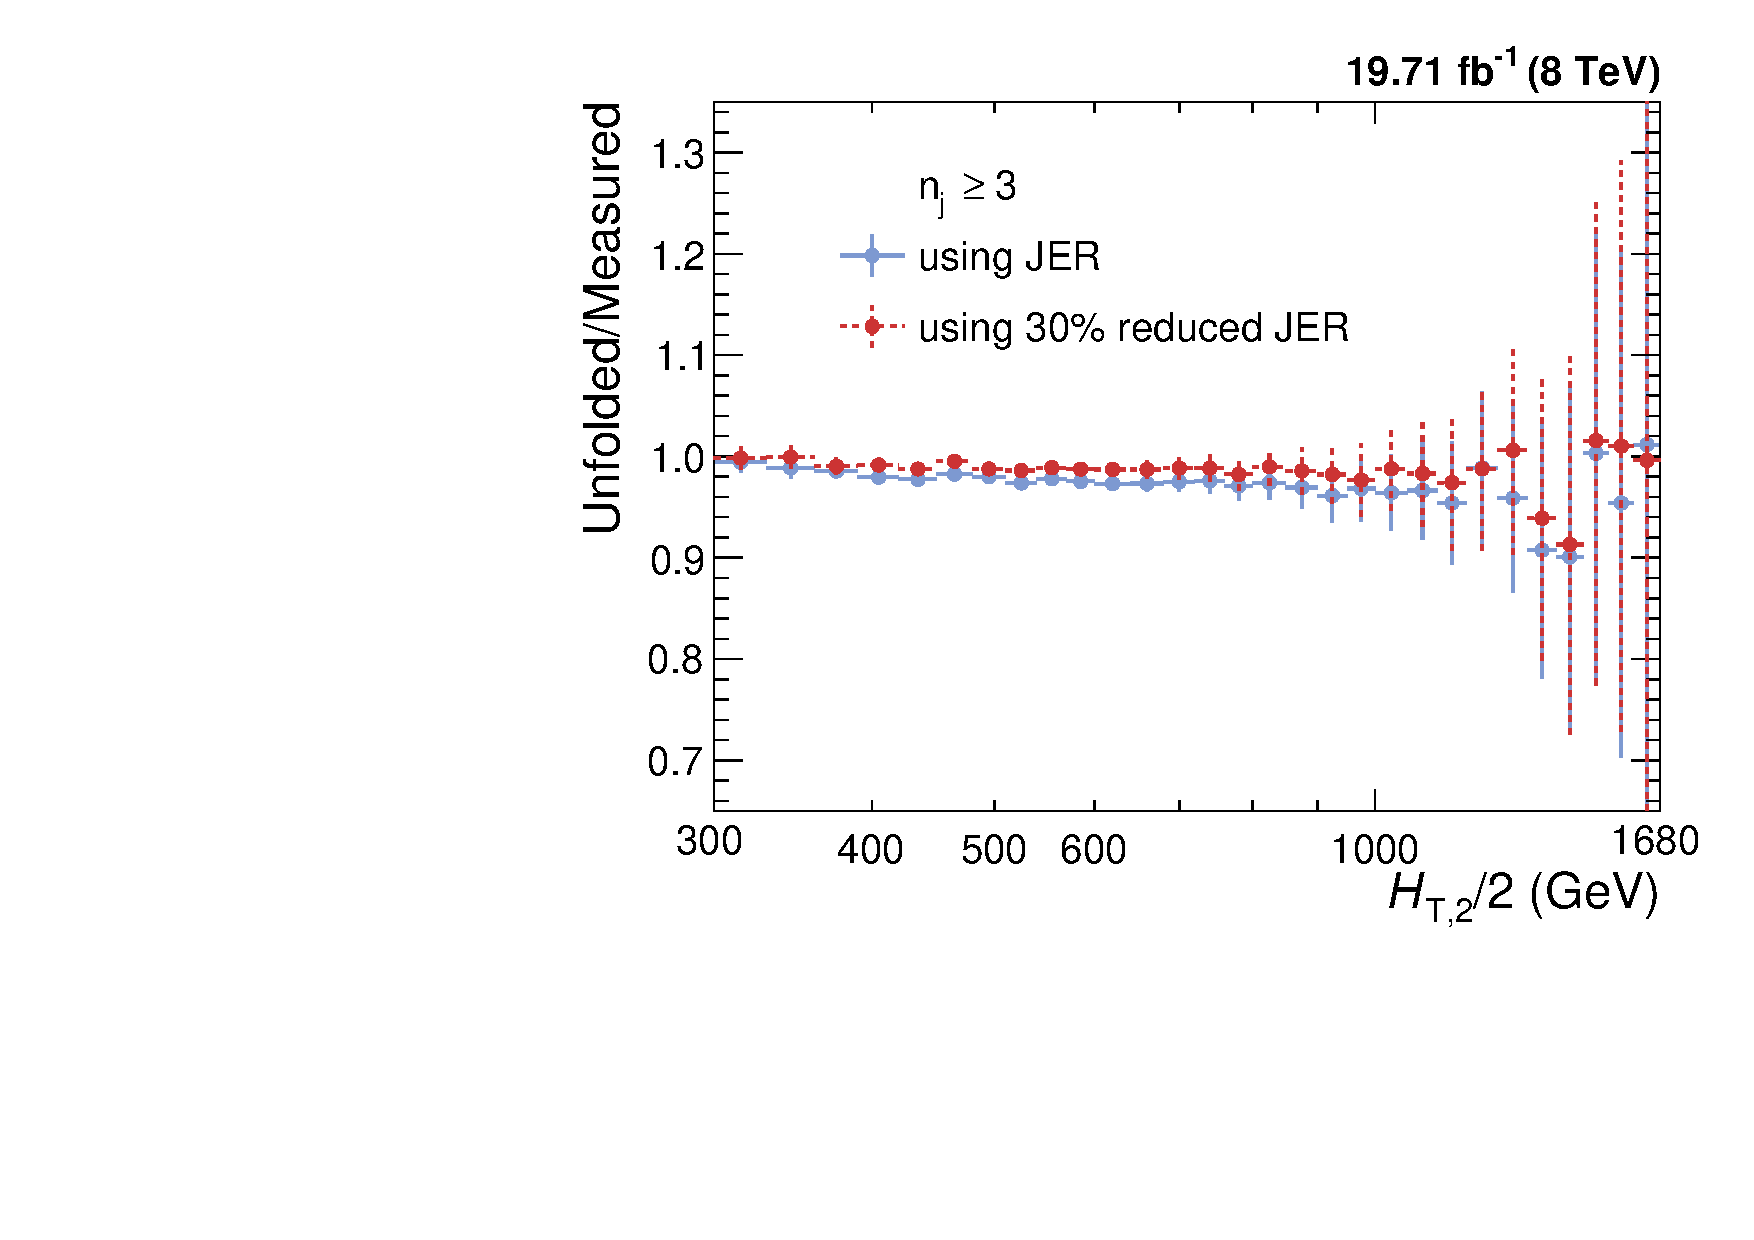
\includegraphics[width=0.51\textwidth]{Plots_HT_2_150/Ratio_Unfolding_data_NLO_3.pdf}\\
 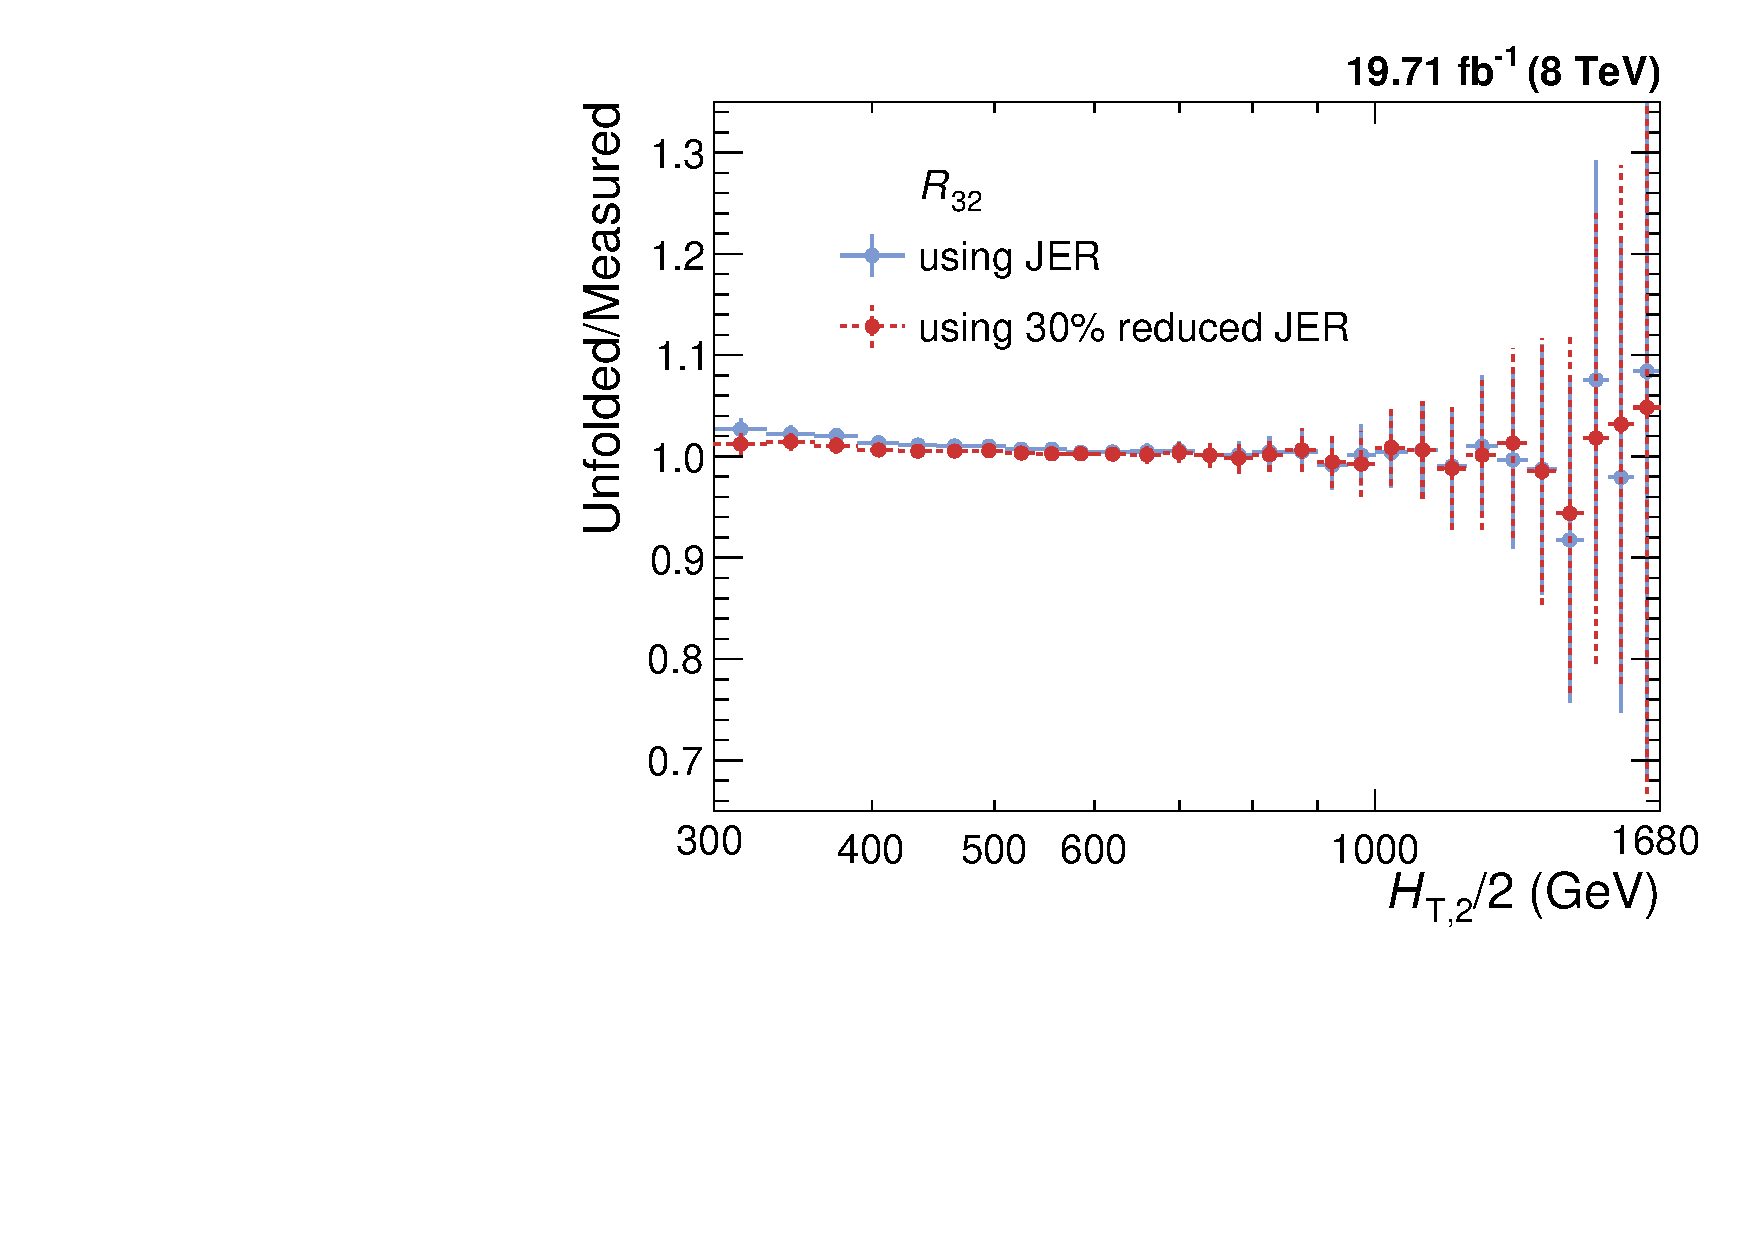
\includegraphics[width=0.51\textwidth]{Plots_HT_2_150/Ratio_Unfolding_data_NLO_ratio32.pdf}
 \caption[The measured differential cross-sections as well as the cross-section ratio \ratio are unfolded as a function of \httwo using the response matrices derived using the Toy Monte Carlo and forward smearing method.]{The measured differential cross-sections as well as the cross-section ratio \ratio are unfolded as a function of \httwo using the response matrices derived using the Toy Monte Carlo and forward smearing method. The unfolded spectrum are compared with that of the measured one for inclusive 2-jet (top left) and 3-jet events cross-sections (right) as well as for \ratio (bottom). The unfolding is done with response matrices using JER (blue solid circles) as well as 30\% reduced JER (red solid circles) for smearing. The difference between both is taken as an additional uncertainty on the unfolded measurement.}
 \label{fig:unfolded_data}
 \end{center}
\end{figure}

\section{Experimental Uncertainties}
\label{sec:exp_unc}
In an experimental measurement of any physical observable, the uncertainties play a key role and hence are important to study in a physics analysis. The uncertainties can be categorized into two types : statistical and systematic. The statistical uncertainties arise due to random fluctuations depending on the number of events. The more the number of events, less is the statistical uncertainty. The systematic uncertainties may be due to known detector effects, model dependence, assumptions made or various corrections applied. In general, if the statistical and systematic uncertainties are uncorrelated, these can be added in quadrature to obtain the total uncertainty on the measurement. In this section, all the experimental uncertainties affecting the measurement of cross-sections and the cross-section ratio \ratio are described. The systematic experimental uncertainties for \ratio are propagated from the cross-sections to the ratio taking into account correlations. Due to this, the systematic uncertainties may cancel for \ratio completely or partially as compared to those for the individual cross-sections.

\subsection{Statistical Uncertainty}
\label{sec:unfolding_stat}
Statistical uncertainty on the measurement is obtained through the unfolding procedure using a toy MC method. The measured data points are smeared within their statistical uncertainties to get the smeared spectrum. Such smeared spectrums are produced million in number and the unfolding is performed multiple times for each smeared spectra. The differences between the unfolded spectrums and the measured one give the statistical uncertainty. The unfolding process introduces more statistical fluctuations which can be observed in Fig.~\ref{fig:stat_unc}. Here the fractional statistical uncertainties of the unfolded data (red line) are compared with those of the measured one (blue line) for \njt~(top left) and \njth~events cross-sections (top right) as well as for the cross-section ratio \ratio (bottom). 

After the unfolding, the final statistical uncertainties become correlated among the bins such that the size of these correlations varies between 10 and 20\%. The correlation (anti-) is more significant for neighbouring bins in \httwo as compared to the far off ones. In Fig.~\ref{fig:corr}, the correlations of the statistical uncertainty after the unfolding can be seen for \njt~(top left) and \njth~events cross-sections (top right) and for the cross-section ratio \ratio (bottom). These correlations must be considered while performing the fits to extract the value of the strong coupling constant, \alpsns. 

\begin{figure}[!ht]
 \begin{center}
 \hspace*{-3mm}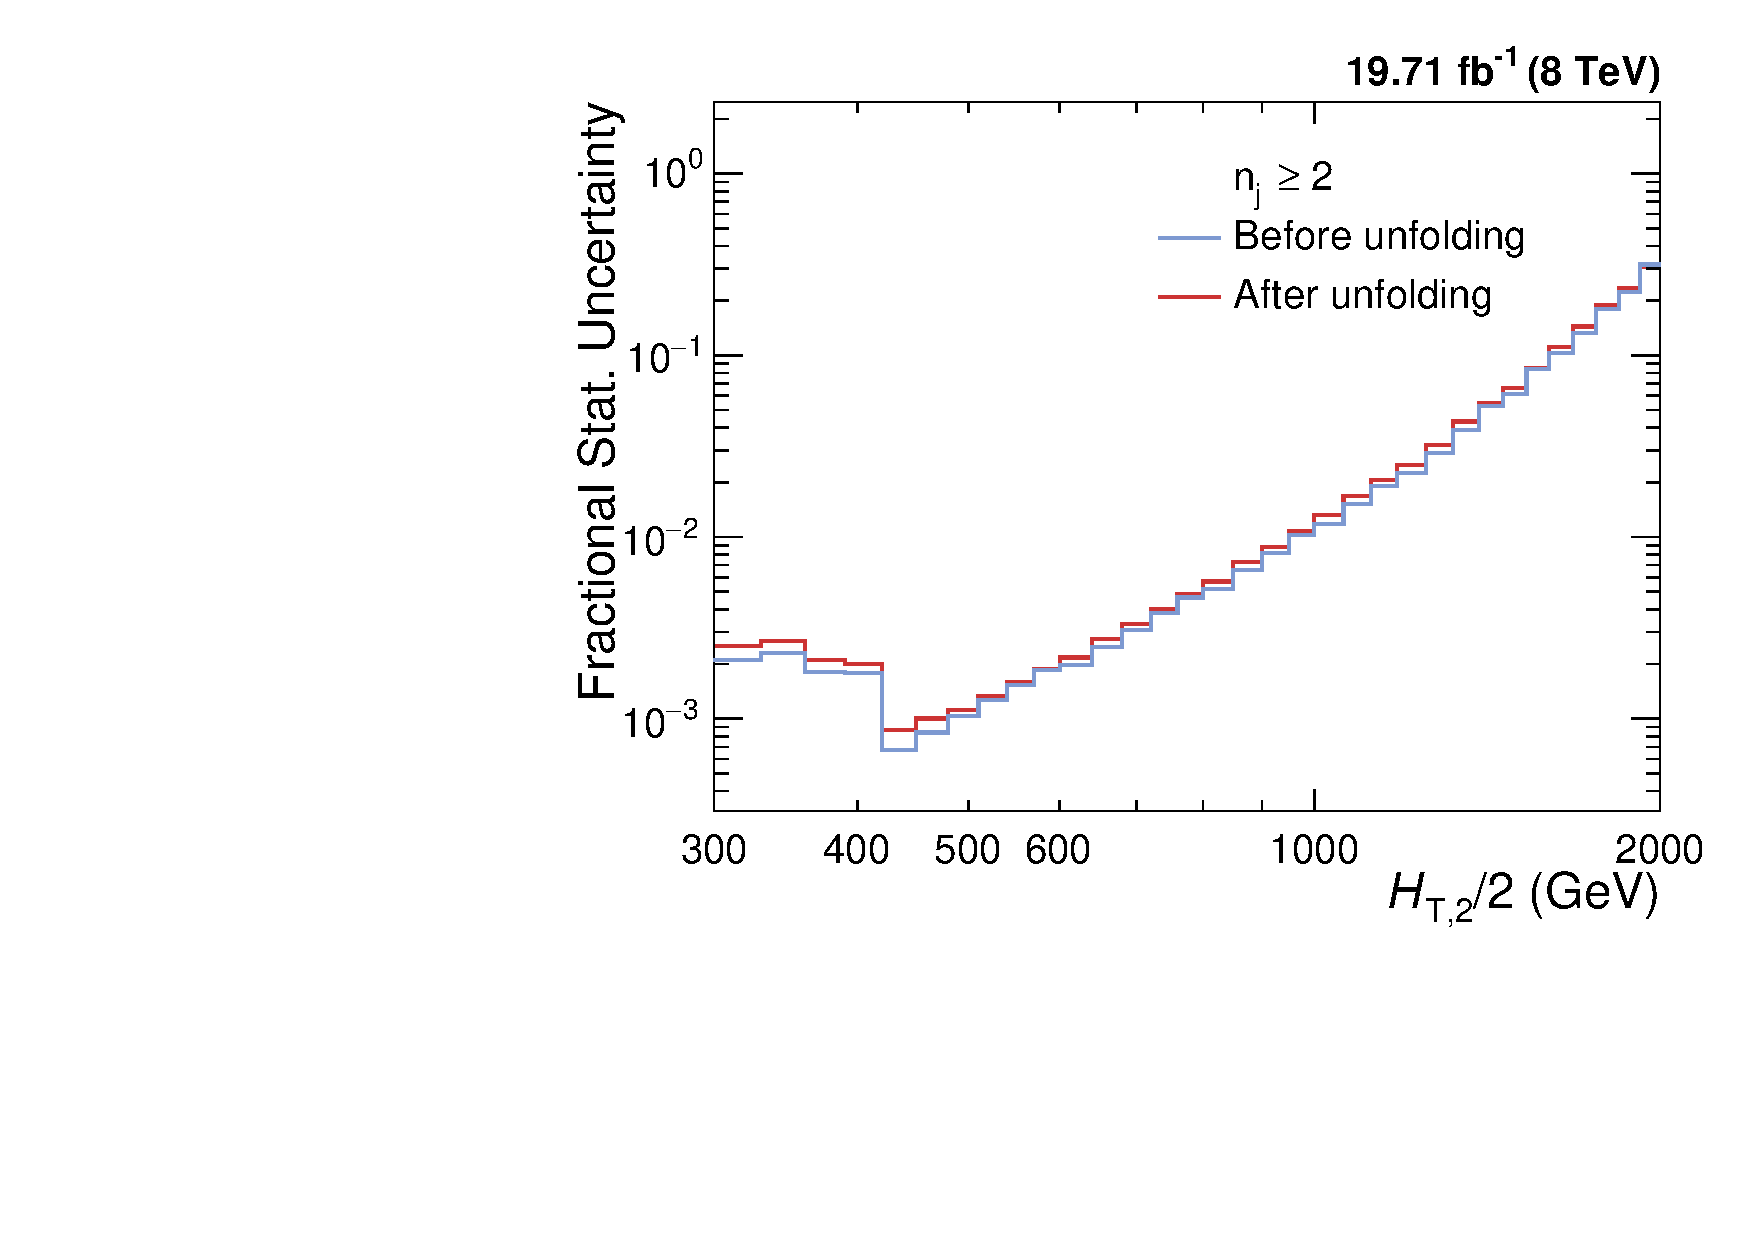
\includegraphics[width=0.51\textwidth]{Plots_HT_2_150/Comparison_stat_unc_2_HT_2_150.pdf}%
 ~~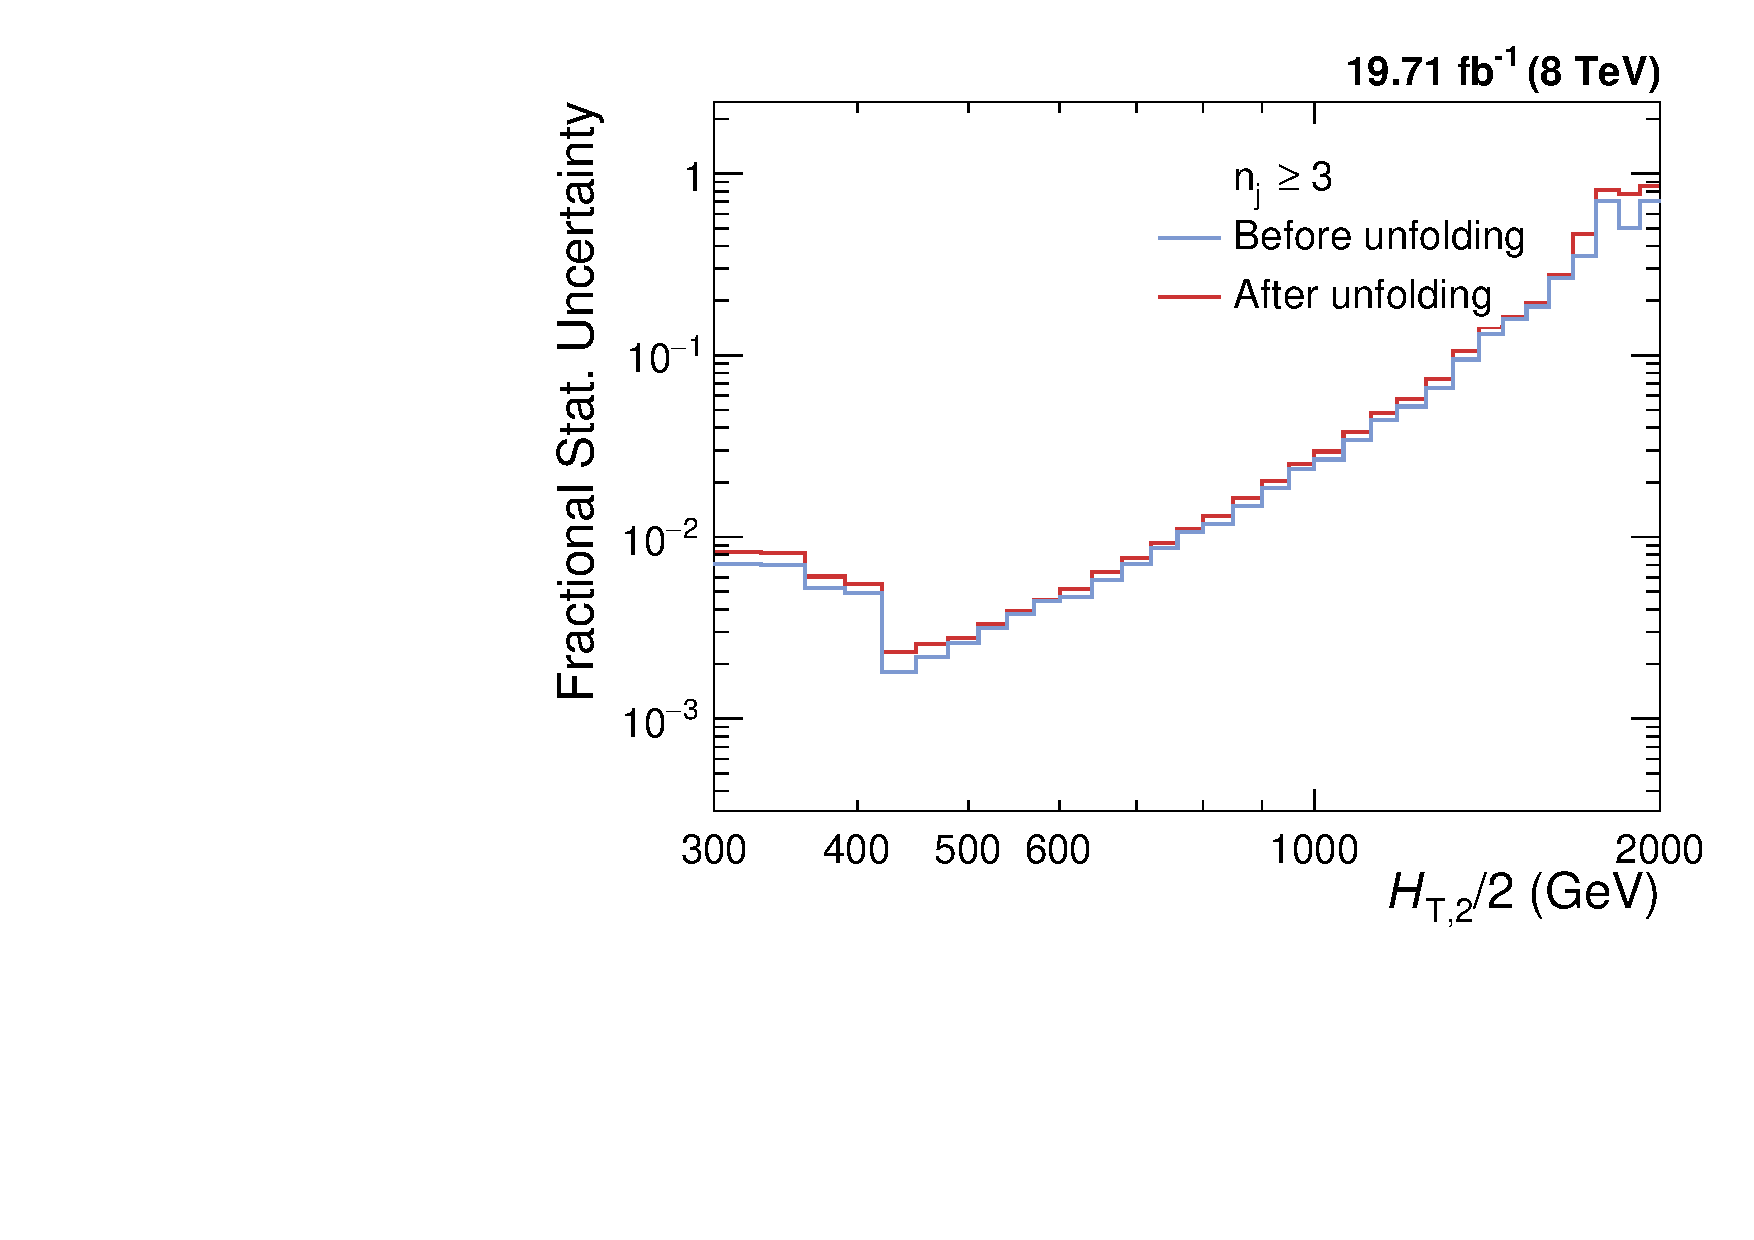
\includegraphics[width=0.51\textwidth]{Plots_HT_2_150/Comparison_stat_unc_3_HT_2_150.pdf}\\
 %\hspace*{-3mm}\includegraphics[width=0.51\textwidth]{Plots_HT_2_150/Comparison_stat_unc_ratio_32_up.pdf}%
 %~~\includegraphics[width=0.51\textwidth]{Plots_HT_2_150/Comparison_stat_unc_ratio_32_down.pdf}
 \includegraphics[width=0.51\textwidth]{Plots_HT_2_150/Comparison_stat_unc_ratio_32_symm.pdf}
 \caption[The fractional statistical uncertainties of the unfolded data are compared with those of the measured one.]{The fractional statistical uncertainties of the unfolded data (red line) are compared with those of the measured one (blue line) for inclusive 2-jet (top left) and 3-jet events cross-sections (top right) as well as for the cross-section ratio \ratio (bottom). After unfolding, the statistical uncertainty increases slightly.}
 \label{fig:stat_unc}
 \end{center}
\end{figure}

\begin{figure}[!h]
 \begin{center}
 \hspace*{-3mm}\includegraphics[width=0.51\textwidth]{Plots_HT_2_150/Correlation_Matrix_NLO_2_ite4.pdf}%
 ~~\includegraphics[width=0.51\textwidth]{Plots_HT_2_150/Correlation_Matrix_NLO_3_ite4.pdf}\\
 \includegraphics[width=0.51\textwidth]{Plots_HT_2_150/Correlation_Matrix_NLO_Ratio_32_ite4.pdf}
 \caption[The unfolding procedure introduces the correlations of the statistical uncertainty through bin migrations.]{The unfolding procedure introduces the correlations of the statistical uncertainty through bin migrations which are shown here for inclusive 2-jet (top left) and and 3-jet events cross-sections (top right) as well as for the cross-section ratio \ratio (bottom). The correlation (anti-) is more significant between neighbouring bins than far-ff ones.}
 \label{fig:corr}
 \end{center}
\end{figure}
 % and in : \\ https://twiki.cern.ch/twiki/bin/viewauth/CMS/ JECUncertaintySources\#Winter14\_uncertainties. 
\subsection{Jet Energy Corrections Uncertainty}
\label{sec:jecs_unc}
As explained in Sec.~\ref{sec:jet_corrections}, the measured jet energy is corrected for a variety of detector effects by using jet energy corrections (JEC). This process introduces uncertainties in the final corrected jet energy. There are 25 mutually independent sources which contribute to JEC. Each source presents a 1$\sigma$ shift and is fully correlated in \pt and $\eta$ but uncorrelated to all other sources. The observable is studied with the nominal values of the jet energy which gives nominal distributions as well as by varying up and down the energy of all jets by the uncertainty. The differences between the nominal distributions and the ones obtained by varying the jet energy gives the uncertainties from each source. The JEC uncertainties can be asymmetric in nature which leads to separate treatment of upwards and downwards variation of each source. The sum in quadrature of uncertainties from all sources gives the total JEC uncertainty. In the current analysis, JEC uncertainties are a dominant source of experimental uncertainty at low \httwo. The JEC uncertainty ranges from 3\% to 10\% for \njt~and from 3\% to 8\% for \njth~events cross-sections measurement. To calculate JEC uncertainty for ratio \rations, the inclusive 2-jet and 3-jet events cross-sections are measured as a function of \httwo by shifting the jet \pt according to the JEC uncertainty for each source of JEC separately. Then the ratio of these cross-sections is taken and the difference of these from the central ratio \rations, gives the JEC uncertainty for \ratio. As expected, JEC uncertainty for \ratio is small as compared to that for individual cross-sections and is about 1 to 2\% over all \httwo bins.

 The sources of JEC considered in the current measurements are : AbsoluteStat, AbsoluteScale, AbsoluteFlavMap, AbsoluteMPFBias, Fragmentation, SinglePionECAL, SinglePionHCAL, FlavorQCD, RelativeJEREC1, RelativeJEREC2, RelativeJERHF, RelativePtBB, RelativePtEC1, RelativePtEC2, RelativePtHF, RelativeFSR, RelativeStatFSR, RelativeStatEC2, RelativeStatHF, PileUpDataMC, PileUpPtRef, PileUpPtBB, PileUpPtEC1, PileUpPtEC2 and PileUpPtHF. The AbsoluteFlavMap uncertainty is exactly zero for the 8 TeV and can be ignored. For the four sources : RelativeJERHF, RelativePtHF, RelativeStatHF, PileUpPtHF, the JEC uncertainty is exactly zero because of $|y|$ \ls 2.5 cut used in the analysis. So only 20 sources contribute to the total JEC uncertainty. The Figs.~\ref{fig:jes1}-\ref{fig:jes3} show the JEC uncertainty from each source separately for inclusive 2-jet (top) and 3-jet events cross-sections (middle) as for cross-section \ratio (bottom). Depending on the origin of sources, they are categorized into four groups which are described below in brief :

\begin{enumerate}
\item {\bf Pileup -} This uncertainty origins from the differences in the transverse momentum between the true offset and the Random Cone method (i.e. essentially difference of pileup inside and outside of jets), in simulated events. This uncertainty is derived from $Z$/$\gamma$\plusn jet, dijet and multijet data using fit procedure to estimate the residual pileup uncertainty after the calibration. 

\item {\bf Relative -} The forward jets are calibrated by the relative $\eta$-dependent corrections using dijet events. The main contribution to the uncertainty comes from jet energy resolution (JER), derived by varying JER scale factors up and down by quoted uncertainties and the initial and final state radiation bias corrections.

\item {\bf Absolute -} A global fit to $Z$/$\gamma$\plusn jet and multijet events gives the absolute calibration of the jet energy scale. The uncertainties are related to the lepton momentum scale for muons in $Z$ ($\rightarrow\mu\mu$)\plusn jet and the single pion response in the HCAL. 

\item {\bf Flavor -} Flavor response differences are studied from simulation by cross-checking the results with quark- and gluon-tagged $\gamma$\plusn jet and $Z$\plusn jet events. These uncertainties are based on \PYTHIASn.4 and \HERWIGPPn 2.3 differences propagated through the data-based calibration method.
\end{enumerate}
The details of the jet energy corrections and uncertainties can be found in \cite{JEC}. 

\subsection{Unfolding Uncertainty}
\label{sec:unfolding_unc}

The unfolding uncertainty is comprised of three uncertainties which are explained as follows :

\begin{enumerate}
\item {\bf Jet Energy Resolution -} The calculation of the jet energy resolution (JER) using simulated \MGP~Monte Carlo events is already explained in Sec.~\ref{sec:Resolution}. As mentioned before, the measured jet transverse momentum (\ptn) in simulated MC events needs to be smeared additionally to match the resolution in data. This smearing is done by using measured scale factors (c$_{central}$) mentioned in Table~\ref{tab:resolution}. It is recommended by \JetMet group that the uncertainty on these measured scaling factors must be taken into account in a physics analysis. Since JER is used in constructing the response matrix which is an input in unfolding procedure, so the uncertainty on scale factors accounts for the unfolding uncertainty. To calculate JER uncertainty, \pt is smeared with two additional sets of scale factors corresponding to varying the factors up and down by one sigma, and corresponding \httwo is calculated. Then again JER is calculated as a function of \httwo using these upwards (c$_{up}$)and downwards (c$_{down}$) variations of the scaling factors. Alternative response matrices are built using the JER with above variations and the unfolding is performed again. The differences of the obtained unfolded spectrums to the nominal ones accounts for a systematic JER uncertainty. 

\item {\bf Model Dependence -} It is explained in Sec.~\ref{sec:funcs} that to obtain the true \httwo spectrum to be used in constructing response matrix using Toy MC method, the fitting of the CT10-NLO predictions is performed with the Function I described in Eq.~\ref{eq:func1}. Using the alternative function, Function II given by Eq.~\ref{eq:func2}, for this fitting and then constructing different response matrix, gives the model dependence of the true \httwo spectrum. The differences in unfolded distributions using the above mentioned two different response matrices gives the model dependence uncertainty.

\item {\bf Additional Uncertainty -} Small nonclosures observed in Fig.~\ref{fig:ratios} introduces a supplementary uncertainty which is attributed by comparison of distributions unfolded using response matrices constructed using JER from simulation with that obtained with a 30\% reduced JER. 
\end{enumerate}

All the three above mentioned uncertainties are added in quadrature to get the total unfolding uncertainty which increases from about 1\% at low \httwo up to 2\% at the high \httwo ends of the cross-sections for both \njt~and \njth~events. This uncertainty account for about less than 1\% for \ratio.

\subsection{Luminosity Measurement Uncertainty}
As discussed in Sec.~\ref{sec:lumi}, the luminosity delivered to CMS detector by LHC in the proton-proton collisions in the year of 2012 is measured by using the silicon pixel cluster counting method \cite{CMS:2013gfa}. The uncertainty related to the integrated luminosity measurement is estimated to be 2.5\% (syst.) and 0.5\% (stat.). This uncertainty propagates directly to any absolute cross-section measurement. Hence, a total systematic uncertainty of 2.6\% is considered across all the \httwo bins. At low \httwons, it is similar in size as the one from JEC. This uncertainty cancels completely for \ratio.

\subsection{Residual Uncertainty}
The small trigger and jet identification inefficiencies account for smaller than 1\% uncertainties on the cross-section measurements \cite{Khachatryan:2016mlc,Chatrchyan:2012bja}. Hence, an uncorrelated residual uncertainty of 1\% is assumed across all \httwo bins for both \njt~and \njth~events cross-sections whereas for \rations, it gets cancel completely.

\subsection{Total Experimental Uncertainty}
After calculating the uncertainties from all the above mentioned sources, the total experimental uncertainty on measurement of cross-sections as well as cross-section ratio \rations, is obtained by adding in quadrature the uncertainties from individual sources. Figure~\ref{fig:exp_unc} shows the experimental uncertainties, from different sources as well as the total uncertainty, affecting the measurement of \njt~(top left) and \njth~events cross-sections (top right) and cross-section ratio \ratio (bottom). The error bars represent the statistical uncertainty obtained after unfolding. The systematic uncertainties due to jet energy corrections (JEC by blue line), luminosity (red dashed line), unfolding (green dashed line) and residual effects (light purple line) are also presented. The uncertainties due to luminosity and residual effects cancel completely in \ratio. The total uncertainty (black dashed line) on the measurements is asymmetric in nature and dominated by the uncertainty due to the jet energy corrections (JEC) at lower \httwo values and by statistical uncertainty at higher \httwo values. 
\begin{figure}[!h]
 \begin{center}
 \hspace*{-3mm}\includegraphics[width=0.51\textwidth]{Plots_HT_2_150/Total_unc_all_2_NLO_add.pdf}%
 ~~\includegraphics[width=0.51\textwidth]{Plots_HT_2_150/Total_unc_all_3_NLO_add.pdf}\\
 \includegraphics[width=0.51\textwidth]{Plots_HT_2_150/Total_Unc_ratio_32_direct_add.pdf}
 \caption[Experimental uncertainties from different sources affecting the measurement of cross-sections and cross-section ratio.]{Experimental uncertainties from different sources affecting the measurement of cross-sections for inclusive 2-jet (top left) and 3-jet events (top right) and cross-section ratio \ratio (bottom). The error bars represent the statistical uncertainty after unfolding. The systematic uncertainties due to jet energy corrections (JEC by blue line), luminosity (red dashed line), unfolding (green dashed line) and residual effects (light purple line) are also presented. The uncertainties due to luminosity and residual effects cancel completely in \ratio. The total uncertainty (black dashed line) is the quadrature sum of the individual sources of uncertainty.}
 \label{fig:exp_unc}
 \end{center}
\end{figure}

The experimental uncertainties from each source as well as total uncertainty are also quoted in Table~\ref{tab:exp_unc_overview}. The values of uncertainties (in \%) from each source as well as total uncertainty, for each \httwo bin, are tabulated in Tables~\ref{tab:exp_unc2},~\ref{tab:exp_unc3} and~\ref{tab:exp_unc_ratio} for \njt~and \njth~events cross-sections and cross-section ratio \rations, respectively. 

\begin{table}[!h]
 \centering
 \caption[An overview of all experimental uncertainties affecting the measurement of cross-sections and the cross-section ratio.]{An overview of all experimental uncertainties affecting the measurement of cross-sections for inclusive 2-jet (left) and 3-jet events (middle) and cross-section ratio \ratio (right). The uncertainties due to luminosity and residual effects cancel completely in \ratio. The total uncertainty is the quadrature sum of the individual sources of uncertainty.}
\label{tab:exp_unc_overview}
  \vspace{2mm}
  \begin{tabular}{llll}
    \hline\hline
     {\bf Uncertainty Source}    & {\bf Inclusive 2-jet} & {\bf Inclusive 3-jet} & {\bf ~~~~\ratio}  \rbthm\\\hline     
     Statistical                 & \ls 1 to 30\%         & \ls 1 to 27\%         & \ls 1 to 28\% \rbtrr\\
     Jet energy corrections (JEC)& ~~~3 to 10\%          & ~~~3 to 8\%           & ~~~1 to 2\%   \rbtrr\\
     Unfolding                   & ~~~1 to 2\%           & ~~~1 to 2\%           & \ls 1\%       \rbtrr\\
     Luminosity                  & ~~~2.6\%              & ~~~2.6\%              & ~~~cancels    \rbtrr\\
     Residual                    & ~~~1\%                & ~~~1\%                & ~~~cancels    \rbtrr\\\hline
     Total                       & ~~~4 to 32\%          & 4 to 28\%             & ~~~1 to 28\%  \rbtrr\\  
  \hline\hline
  \end{tabular}
\end{table}
\begin{comment}
     {\bf Statistical}  & \ls 1 to 30\% & \ls 1 to 27\% & \ls 1 to 28\% \rbtrr\\
     {\bf \textcolor{blue2}{Jet energy corrections (JEC)}}  & 3 to 10\% & 3 to 8\% & 1 to 2\%\rbtrr\\
     {\bf \textcolor{green}{Unfolding}} & 1-2\% & 1-2\% & \ls 1\% \rbtrr\\
     {\bf \textcolor{myred}{Luminosity}} & 2.6\% & 2.6\% & cancels\rbtrr\\
     {\bf \textcolor{lightpurple}{Residual}} & 1\% & 1\% & cancels \rbtrr\\\hline
     {\bf Total} & 4 to 32\% & 4 to 28\% & 1 to 28\% \rbtrr\\
\end{comment}

The complete data analysis of the differential inclusive 2-jet and 3-jet events cross-sections as well as their ratio \ratio has been presented as a function of \httwo. The measured spectrums after correcting for detector effects through the unfolding procedure, are compared with the next-to-leading order (NLO) pQCD calculations in the next chapter. 
